%%%%%%%%%%%%%%%%%%%%%%%%%%%%%%%%%%%%%%%%%
% Masters/Doctoral Thesis 
% LaTeX Template
% Version 2.1 (2/9/15)
%
% This template has been downloaded from:
% http://www.LaTeXTemplates.com
%
% Version 2.0 major modifications by:
% Vel (vel@latextemplates.com)
%
% Original authors:
% Steven Gunn  (http://users.ecs.soton.ac.uk/srg/softwaretools/document/templates/)
% Sunil Patel (http://www.sunilpatel.co.uk/thesis-template/)
%
% License:
% CC BY-NC-SA 3.0 (http://creativecommons.org/licenses/by-nc-sa/3.0/)
%
%%%%%%%%%%%%%%%%%%%%%%%%%%%%%%%%%%%%%%%%%

%----------------------------------------------------------------------------------------
%	PACKAGES AND OTHER DOCUMENT CONFIGURATIONS
%----------------------------------------------------------------------------------------

\documentclass[
12pt, % The default document font size, options: 10pt, 11pt, 12pt
oneside, % Two side (alternating margins) for binding by default, uncomment to switch to one side
english, % ngerman for German
onehalfspacing, % Single line spacing, alternatives: onehalfspacing or doublespacing
%draft, % Uncomment to enable draft mode (no pictures, no links, overfull hboxes indicated)
%nolistspacing, % If the document is onehalfspacing or doublespacing, uncomment this to set spacing in lists to single
%liststotoc, % Uncomment to add the list of figures/tables/etc to the table of contents
%toctotoc, % Uncomment to add the main table of contents to the table of contents
%parskip, % Uncomment to add space between paragraphs
]{MastersDoctoralThesis} % The class file specifying the document structure

\usepackage[utf8]{inputenc} % Required for inputting international characters
\usepackage[T1]{fontenc} % Output font encoding for international characters

\usepackage{palatino} % Use the Palatino font by default

\usepackage[backend=bibtex,sorting=none]{biblatex} % User the bibtex backend with the authoryear citation style (which resembles APA)

\addbibresource{example.bib} % The filename of the bibliography
\DeclareNameAlias{sortname}{last-first}
\DeclareNameAlias{default}{last-first}

\usepackage{amsfonts}
\usepackage[cmex10]{amsmath}
\usepackage{comment}
\usepackage{times}
\usepackage{amsmath}
\usepackage{changepage}
\usepackage{amssymb}
\usepackage{listings}
\usepackage{mathtools} 
\usepackage{color}
\usepackage{paralist}
\usepackage{lastpage} % Required to determine the last page for the footer
\usepackage{courier}
\usepackage{textcomp}
\usepackage{algorithm2e}
\usepackage{setspace}
\usepackage{listings}
\AtBeginDocument{\DeclareCaptionSubType{lstlisting}}
\usepackage[centerlast,small,sc]{caption}
\usepackage{subcaption}
\setlength{\captionmargin}{50pt}


\usepackage{todonotes}
\newcommand{\todojc}[1]{\todo[inline]{JC: #1}}

\definecolor{mygreen}{rgb}{0,0.6,0}
\definecolor{mygray}{rgb}{0.5,0.5,0.5}
\definecolor{mymauve}{rgb}{0.58,0,0.82}
\definecolor{mylisting}{rgb}{1,0.98,0.756}

\lstset{ %
  backgroundcolor=\color{mylisting},   % choose the background color; you must add \usepackage{color} or \usepackage{xcolor}
  basicstyle=\footnotesize\ttfamily,        % the size of the fonts that are used for the code
  breakatwhitespace=false,         % sets if automatic breaks should only happen at whitespace
  breaklines=true,                 % sets automatic line breaking
  captionpos=t,                    % sets the caption-position to bottom
  commentstyle=\color{mygreen},    % comment style
  deletekeywords={...},            % if you want to delete keywords from the given language
  escapeinside={\%*}{*)},          % if you want to add LaTeX within your code
  extendedchars=true,              % lets you use non-ASCII characters; for 8-bits encodings only, does not work with UTF-8
  frame=single,                    % adds a frame around the code
  keepspaces=true,                 % keeps spaces in text, useful for keeping indentation of code (possibly needs columns=flexible)
  keywordstyle=\color{blue},       % keyword style
  language=Java,                 % the language of the code
  morekeywords={*,...},            % if you want to add more keywords to the set
  numbers=left,                    % where to put the line-numbers; possible values are (none, left, right)
  numbersep=5pt,                   % how far the line-numbers are from the code
  numberstyle=\tiny\color{mygray}, % the style that is used for the line-numbers
  rulecolor=\color{black},         % if not set, the frame-color may be changed on line-breaks within not-black text (e.g. comments (green here))
  showspaces=false,                % show spaces everywhere adding particular underscores; it overrides 'showstringspaces'
  showstringspaces=false,          % underline spaces within strings only
  showtabs=false,                  % show tabs within strings adding particular underscores
  stepnumber=2,                    % the step between two line-numbers. If it's 1, each line will be numbered
  stringstyle=\color{mymauve},     % string literal style
  tabsize=2,                       % sets default tabsize to 2 spaces
%   title=\lstname ,                  % show the filename of files included with \lstinputlisting; also try caption instead of title
  moredelim=**[is][\color{red}]{@!}{@!},
  lineskip={-1.5pt}
}



\newcommand{\includecode}[4]{\lstinputlisting[captionpos=t,language=#4,caption={#3},label={#2}]{code/#1}}

\newcommand{\addfigure}[4]{
\begin{figure}[h]
	\centering
	\includegraphics[scale=#1]{#2}
	\caption{#3}
	\label{#4}
\end{figure}
}

\newcommand{\printCode}[3]{
	\begin{figure}[h]
	\captionsetup{type=lstlisting} 
	\caption{#2}
	\begin{sublstlisting}[t]{0.47\linewidth}
	\caption{C code}
	\lstinputlisting[captionpos=t,language=C]{code/#1.c}
	\end{sublstlisting} \hfill
	\begin{sublstlisting}[t]{0.47\linewidth}
	\caption{Assembly Code}
	\lstinputlisting[captionpos=t,language=C]{code/#1.s}
	\end{sublstlisting}
	\label{#3}
	\end{figure}
}




%----------------------------------------------------------------------------------------
%	THESIS INFORMATION
%----------------------------------------------------------------------------------------

\thesistitle{Thesis Title} % Your thesis title, this is used in the title and abstract, print it elsewhere with \ttitle
\supervisor{Brett H. \textsc{Meyer}} % Your supervisor's name, this is used in the title page, print it elsewhere with \supname
\examiner{} % Your examiner's name, this is not currently used anywhere in the template, print it elsewhere with \examname
\degree{Master of Engineering} % Your degree name, this is used in the title page and abstract, print it elsewhere with \degreename
\author{Jonah \textsc{Caplan}} % Your name, this is used in the title page and abstract, print it elsewhere with \authorname
\addresses{} % Your address, this is not currently used anywhere in the template, print it elsewhere with \addressname

\subject{Electrical Engineering} % Your subject area, this is not currently used anywhere in the template, print it elsewhere with \subjectname
\keywords{} % Keywords for your thesis, this is not currently used anywhere in the template, print it elsewhere with \keywordnames
% \university{\href{http://www.university.com}{University Name}} % Your university's name and URL, this is used in the title page and abstract, print it elsewhere with \univname
\university{McGill University}
\department{Electrical and Computer Engineering} % Your department's name and URL, this is used in the title page and abstract, print it elsewhere with \deptname
\group{Reliable Silicon Systems Lab} % Your research group's name and URL, this is used in the title page, print it elsewhere with \groupname
\faculty{Faculty of Engineering} % Your faculty's name and URL, this is used in the title page and abstract, print it elsewhere with \facname

\hypersetup{pdftitle=\ttitle} % Set the PDF's title to your title
\hypersetup{pdfauthor=\authorname} % Set the PDF's author to your name
\hypersetup{pdfkeywords=\keywordnames} % Set the PDF's keywords to your keywords

\begin{document}

\frontmatter % Use roman page numbering style (i, ii, iii, iv...) for the pre-content pages

\pagestyle{plain} % Default to the plain heading style until the thesis style is called for the body content

%----------------------------------------------------------------------------------------
%	TITLE PAGE
%----------------------------------------------------------------------------------------

\begin{titlepage}
\begin{center}

\textsc{\LARGE \univname}\\[1.5cm] % University name
\textsc{\Large Masters Thesis}\\[0.5cm] % Thesis type

\HRule \\[0.4cm] % Horizontal line
{\huge \bfseries \ttitle}\\[0.4cm] % Thesis title
\HRule \\[1.5cm] % Horizontal line
 
\begin{minipage}{0.4\textwidth}
\begin{flushleft} \large
\emph{Author:}\\
\authorname % Author name - remove the \href bracket to remove the link
\end{flushleft}
\end{minipage}
\begin{minipage}{0.4\textwidth}
\begin{flushright} \large
\emph{Supervisor:} \\
\supname % Supervisor name - remove the \href bracket to remove the link  
\end{flushright}
\end{minipage}\\[3cm]
 
\large \textit{A thesis submitted in fulfilment of the requirements\\ for the degree of \degreename}\\[0.3cm] % University requirement text
\textit{in the}\\[0.4cm]
\groupname\\\deptname\\[2cm] % Research group name and department name
 
{\large \today}\\[4cm] % Date
%\includegraphics{Logo} % University/department logo - uncomment to place it
 
\vfill


Copyright \textsf{\textcopyright} \ 2016 Jonah Caplan

\end{center}

\end{titlepage}



%----------------------------------------------------------------------------------------
%	DECLARATION PAGE
%----------------------------------------------------------------------------------------

% \begin{declaration}
% \addchaptertocentry{\authorshipname}
% 
% \noindent I, \authorname, declare that this thesis titled, \enquote{\ttitle} and the work presented in it are my own. I confirm that:
% 
% \begin{itemize} 
% \item This work was done wholly or mainly while in candidature for a research degree at this University.
% \item Where any part of this thesis has previously been submitted for a degree or any other qualification at this University or any other institution, this has been clearly stated.
% \item Where I have consulted the published work of others, this is always clearly attributed.
% \item Where I have quoted from the work of others, the source is always given. With the exception of such quotations, this thesis is entirely my own work.
% \item I have acknowledged all main sources of help.
% \item Where the thesis is based on work done by myself jointly with others, I have made clear exactly what was done by others and what I have contributed myself.\\
% \end{itemize}
%   
% \noindent Signed:\\
% \rule[0.5em]{25em}{0.5pt} % This prints a line for the signature
%  
% \noindent Date:\\
% \rule[0.5em]{25em}{0.5pt} % This prints a line to write the date
% \end{declaration}
% 
% \cleardoublepage



%----------------------------------------------------------------------------------------
%	ABSTRACT PAGE
%----------------------------------------------------------------------------------------

\begin{abstract}
\addchaptertocentry{\abstractname} % Add the abstract to the table of contents

The Thesis Abstract is written here (and usually kept to just this page). The page is kept centered vertically so can expand into the blank space above the title too\ldots

\end{abstract}

%----------------------------------------------------------------------------------------
%	ACKNOWLEDGEMENTS
%----------------------------------------------------------------------------------------

\begin{acknowledgements}
\addchaptertocentry{\acknowledgementname} % Add the acknowledgements to the table of contents

% Parents: Michael and Wendy Caplan
% Collaborators: Zaid Al-Bayati, Harsh Aurora, Ataias, Mojing, Georgi
% Supervisor: Brett H. Meyer
% Rest of my family and friends: few, proud, patient


\end{acknowledgements}

%----------------------------------------------------------------------------------------
%	LIST OF CONTENTS/FIGURES/TABLES PAGES
%----------------------------------------------------------------------------------------

\tableofcontents % Prints the main table of contents

\listoffigures % Prints the list of figures

\listoftables % Prints the list of tables

%----------------------------------------------------------------------------------------
%	ABBREVIATIONS
%----------------------------------------------------------------------------------------

\begin{abbreviations}{ll} % Include a list of abbreviations (a table of two columns)

\textbf{LAH} & \textbf{L}ist \textbf{A}bbreviations \textbf{H}ere\\
\textbf{WSF} & \textbf{W}hat (it) \textbf{S}tands \textbf{F}or\\

\end{abbreviations}

%----------------------------------------------------------------------------------------
%	DEDICATION
%----------------------------------------------------------------------------------------

% \dedicatory{For/Dedicated to/To my\ldots}  

%----------------------------------------------------------------------------------------
%	THESIS CONTENT - CHAPTERS
%----------------------------------------------------------------------------------------

\mainmatter % Begin numeric (1,2,3...) page numbering

\pagestyle{thesis} % Return the page headers back to the "thesis" style

% Include the chapters of the thesis as separate files from the Chapters folder
% Uncomment the lines as you write the chapters

% 

% Chapter Template

\chapter{Introduction} % Main chapter title

\label{c:intro} % Change X to a consecutive number; for referencing this chapter elsewhere, use \ref{ChapterX}

%----------------------------------------------------------------------------------------
%	SECTION 1
%----------------------------------------------------------------------------------------


	Embedded system design lies at the intersection of several fields: software design, signal processing, control theory, harware design, etc. 
	Often the hardware and software in these systems must be specified and designed in parallel due to increasing time-to-market pressures. 
	FPGA prototyping and virtual platform simulation are opening up new possibilities for effective hardware-software codesign strategies. 
	As a result, most application engineers in large industries such as automative are managing the complexity of the design space and the difficulties in writing and debugging dependable code by moving towards model based design and code generation. 
	Code generation also has the benefit of reducing platform specific dependencies and increasing code reuseability. 
	A sigificant portion of the millions of lines of code in modern cars will be generated automatically from models.

	The use of multicore architectures in real-time systems further complicates the design process. 
	Multicore engine control units (ECUs) have only appeared on the market in the last couple of years (e.g. Infineon Aurix product line). 
	Support for multicore architectures by software providers in real-time model based design (e.g. LabVIEW, Simulink, Esterel) is very limited or non-existent.
	Multicore architectures are of particular interest in providing more efficient solutions to transient fault management in mixed criticality systems where resources are shared by both safety critical and non-safety critical functions. 

	In previous work we have designed and implemented a prototype multicore architecture on an FPGA using Nios soft cores and fingerprinting to detect errors caused by transient faults. 
	Programming with fingerprinting requires a lot of tedious detail work and is error-prone and difficult.
% 	The development of high caliber research implementations of software systems using the new platform intersects several fields: control systems, embedded software, digital design, code profiling, and schedulability analysis. 
% 	Code generation allows abstract models to be implemented at a much faster rate.
	This project provides a baseline framework that allows quick porting of code to the multicore system. 
	
\section{Contributions}

	This project specifically contributes the following infrastructure to support the goal of reference implementation development:
	\begin{itemize}
	  \item A novel schedulability analysis for mixed criticality fault tolerant multicore systems.
	  \item A code generation framework for porting code quickly to a Nios based multicore system.
	  \item Profiling and design space exploration tools to support automation of low level design parameters for code generation from high level functional configuration requirements.
	\end{itemize}
	
	In general, each component is fairly naive in its implementation and assumptions. 
	The purpose of this project is to deliver a framework with well defined interfaces between discrete aspects of the design problem in order to facilitate future collaboration and research development. 
	The most pressing long term issues are the discrepency between high level schedulability models and actual system performance as well as generating high quality static worst case execution time estimates.
	We believe the starting point for significant work in this area requires a model based framework that speeds up the implementation cycle to compare measurements of actual systems with the models used to design them.
	Code generation further allows participants to address specific aspects of the problem without being experts in all overlapping domains.

\section{Outline}
% 	The thesis chapters are as follows:
% 	\begin{itemize}
% 	  \item Chapter~\ref{c:background} reviews prior work and related concepts including mixed criticality systems, on demand redundancy, fingerprinting, Simulink, and Open Virtual Platforms.
% 	  \item Chapter~\ref{c:tool-arch} presents an overview of the entire tool chain and the workflow for each component. 
% 	  \item Chapter~\ref{c:prof} discusses the profiling tool with special emphasis on the reconstruction of control flow graphs and expressions from the assembly code. These representations are then analyzed in further detail to infer maximum number of loop iterations.
% 	  \item Chapter~\ref{c:sched} discusses a schedulability analysis based on AMC-rtb is presented that supports fault-tolerant cores (e.g. lockstep) as well as several varieties of on-demand redundancy in multicore systems. The analysis is then integrated into a design space exploration engine that maps tasks onto platforms and decides which technique to use for each task.
% 	  \item Chapter~\ref{c:soft-impl} discusses the implementation model of the fault tolerant system in more detail.
% 	  \item Chapter~\ref{c:code-gen} discusses the code generation tool that produces code for all cores in the platform based on the mapping results. The tool also automatically generates and configures the board support package (BSP) using the Nios SBT tools.
% 	  \item Chapter~\ref{c:related} discusses related work. 
% 	  \item Chapter~\ref{c:concl} discusses possible directions for future work and presents our conclusion.
% 	\end{itemize}
	Chapter~\ref{c:background} reviews prior work and related concepts including mixed criticality systems, on demand redundancy, fingerprinting, Simulink, and Open Virtual Platforms. 
	Chapter~\ref{c:tool-arch} presents an overview of the entire tool chain and the workflow for each component. 
	Chapter~\ref{c:prof} discusses the profiling tool with special emphasis on the reconstruction of control flow graphs and expressions from the assembly code. 
	These representations are then analyzed in further detail to infer maximum number of loop iterations. 
	Chapter~\ref{c:sched} discusses a schedulability analysis based on AMC-rtb is presented that supports fault-tolerant cores (e.g. lockstep) as well as several varieties of on-demand redundancy in multicore systems. 
	The analysis is then integrated into a design space exploration engine that maps tasks onto platforms and decides which technique to use for each task. C
	hapter~\ref{c:soft-impl} discusses the implementation model of the fault tolerant system in more detail. 
	Chapter~\ref{c:code-gen} discusses the code generation tool that produces code for all cores in the platform based on the mapping results. 
	The tool also automatically generates and configures the board support package (BSP) using the Nios SBT tools. 
	Chapter~\ref{c:related} discusses related work. 
	Chapter~\ref{c:concl} discusses possible directions for future work and presents our conclusion.

% Chapter Template

\chapter{Background} % Main chapter title

\label{c:background} % Change X to a consecutive number; for referencing this chapter elsewhere, use \ref{ChapterX}


	This chapter presents relevant background information on several topics for this thesis. 
	First, Section~\ref{s:mixedcriticality} reviews \emph{mixed criticality} and the scheduling theory which is the basis for Chapter~\ref{c:prof}. 
	Section~\ref{s:odr} reviews \emph{on-demand redundancy}, a type of error detection technique geared towards mixed criticality systems with fault-tolerance requirements. 
	Sections~\ref{s:nios} and \ref{s:hd} more specifically reviews the target platform for code generation and how \emph{fingerprinting} is used to detect errors to achieve on-demand redundancy.
	Section~\ref{s:ovp} reviews the virtual modeling tools used to develop software for the target platform.
	Section~\ref{s:simulink} discusses Simulink and the limitations imposed on Simulink generated code for the work in this thesis.
	
%----------------------------------------------------------------------------------------
%	SECTION 1
%----------------------------------------------------------------------------------------

\section{Mixed Criticality}
\label{s:mixedcriticality}
	Mixed criticality systems share resources between safety-critical tasks where failure can result in expensive damage or harm to users (e.g. x-by-wire), and non-safety critical tasks (e.g. infotainment). 
	Many industries such as automotive and avionics are trying to integrate low criticality (LO) and high criticality (HI) tasks onto the same processors.
	Mixed criticality scheduling (MCS) is the analysis of scheduling algorithms that provide safety guarantees to HI tasks in the presence of LO tasks \cite{burns2013mixed}.
	
	Adaptive mixed criticality (AMC), and more specifically the response time bound analysis (AMC-rtb) \cite{baruah2011response} is the baseline for much work in MCS. 
	AMC models applications as a set of as independent periodic tasks with fixed deadlines and periods (often assumed to be the same).
	Furthermore, HI tasks are assigned an optimistic and pessimistic worst case execution time (WCET). 
	The system is initially in a LO mode, where all tasks meet their deadline as long as they respect their optimistic execution time.
	Runtime mechanisms are put in place that detect when a task has exceeded its budget.
	In this case, the system transitions into the HI mode and drops as many LO tasks as necessary to guarantee that all HI tasks still have enough time to meet their deadlines provided their pessimistic execution times. 
	
	The formal notation for AMC is:
	\begin{itemize}
	  \item $\tau_i$: task $i$
	  \item $C_i(LO)$: LO mode WCET of $\tau_i$
	  \item $C_i(HI)$: HI mode WCET of $\tau_i$
	  \item $L_i$: Criticality of $\tau_i$ (LO or HI)
	  \item $T$: Period of $\tau_i$
	  \item $R_i$: Response time of $\tau_i$
	\end{itemize}

	Rate-monotonic scheduling assigns the highest priority to the task with the smallest period. Criticality inversion, depicted in Figure~\ref{f:responsetime}, is when LO tasks are able to preempt HI tasks. Priority inversion is desirable in mixed criticality systems if LO tasks have shorter periods than HI tasks \cite{baruah2011response}. However, this necessitates the runtime monitoring and mode change in case the effects of LO tasks risk causing a HI task to miss a deadline.

\addfigure{0.7}{responsetime.pdf}{Example of criticality inversion in mixed criticality system using rate monotonic scheduling.}{f:responsetime}

AMC-rtb analysis consists of two equations for the response time of each task in the LO and HI mode:
\begin{equation}
R_i^{(LO)}= C_i(LO)+\sum_{j \in hp(i)}\Big\lceil\frac{R_i^{(LO)}}{T_j}\Big\rceil \cdot C_j(LO)
\label{eq:mode1}
\end{equation}
\begin{equation}
\begin{aligned}
R_i^{(HI)} &  = C_i(HI)+\sum_{j \in hpH(i)}\Big\lceil\frac{R_i^{(HI)}}{T_j}\Big\rceil \cdot C_j(HI) \\
&  +\sum_{k \in hpL(i)}\Big\lceil\frac{R_i^{(LO)}}{T_k}\Big\rceil \cdot C_k(LO)
\end{aligned}
\label{eq:mode2}
\end{equation}
where $hp(i)$ is the set of tasks with higher priority than $\tau_i$, $hpH(i)$ is the set of tasks with higher priority than $\tau_i$ that continue to execute in the HI mode, and $hpL(i)$ is the set of tasks with higher priority than $\tau_i$ that only execute in the LO mode.

	Equation~\ref{eq:mode1} defines the response time $R_i$ to be the LO mode WCET $C_i(LO)$ in addition to the worst-case amount of time all higher priority tasks $hp(i)$ may preempt $\tau_i$. 
	Equation~\ref{eq:mode2} shows that in the HI mode, the response time takes into account preemptions of $hpH(i)$ that are assumed to run for their pessimistic $C_i(HI)$. 
	Dropped tasks ($hpL(i)$) may still have preempted $\tau_i$ prior to the mode change and the third term in Equation~\ref{eq:mode2} models the carry-over effects.

% \section{Transient Faults}


\section{On-Demand Redundancy}
\label{s:odr}

	Transient faults or soft errors occur when environmental radation causes voltage spikes in digital circuits \cite{Baumann:05}. 
	Transient faults must be accounted for in safety critical applications despite their rare occurrence due to the catastrophic consequences that may occur such as loss of life.
	All references to faults in this thesis refer only to transient faults whether or not explicitly stated. 
	This thesis is specifically focused on transient faults in the register files of processors. 
	Network \cite{radetzki2013methods} and memory \cite{Baumann:05} are also susceptible to transient faults however they are assumed to be dealt with by other mechanisms.


% 	Current solutions to transient errors typically rely on replication of entire boards. 
	Lockstep execution \cite{baleani2003fault} is the de facto method of error detection in ECUs \cite{infineon2014aurix,freescale2014qorivva,renesas2016lockstep}. Lockstep execution, shown in Figure~\ref{f:lockstep}, consists of two cores executing the same code in parallel. 
	Lockstep implements redundancy at a very fine granularity as each store instruction is compared in hardware before being released to the bus. 
	If the store output does not match then some rollback procedure must be implemented or else the processors are restarted. 
	It is only possible to detect an error with two processors. 
	Correction can be implemented with three processors by majority vote. 
	Lockstep cores are difficult to build and scale due to the precise synchronization required.

	Lockstep execution is problematic in mixed criticality systems because it is not possible to \emph{decouple} the cores (i.e. use them to run different code independently). 
	It is inefficient to run mixed criticality applications on a pair of \emph{statically coupled} lockstep cores because not all tasks necessarily require protection against transient faults. 
	In Figure~\ref{f:lockstep}, both non-critical tasks (blue) as well as critical tasks (red) must execute on two cores at all times. 	
	The four physical cores operate as two logical nodes regardless of the workload.

	On-Demand redundancy (ODR) \cite{Meyer:CASES11,fu2013demand}, or dynamic core coupling \cite{lafrieda2007utilizing}, proposes the \emph{dynamic} coupling of cores in the system. 
	Only high criticality tasks requiring error detection will use two processors to execute redundant threads. 
	Figure~\ref{f:odr} shows how LO tasks are no longer forced to execute on two cores, thus freeing up resources to execute more tasks on the same number of cores.


\begin{figure}
\captionsetup[subfigure]{singlelinecheck=false}
\centering
\subcaptionbox{Lockstep execution \label{f:lockstep}}[0.45\textwidth]
{
    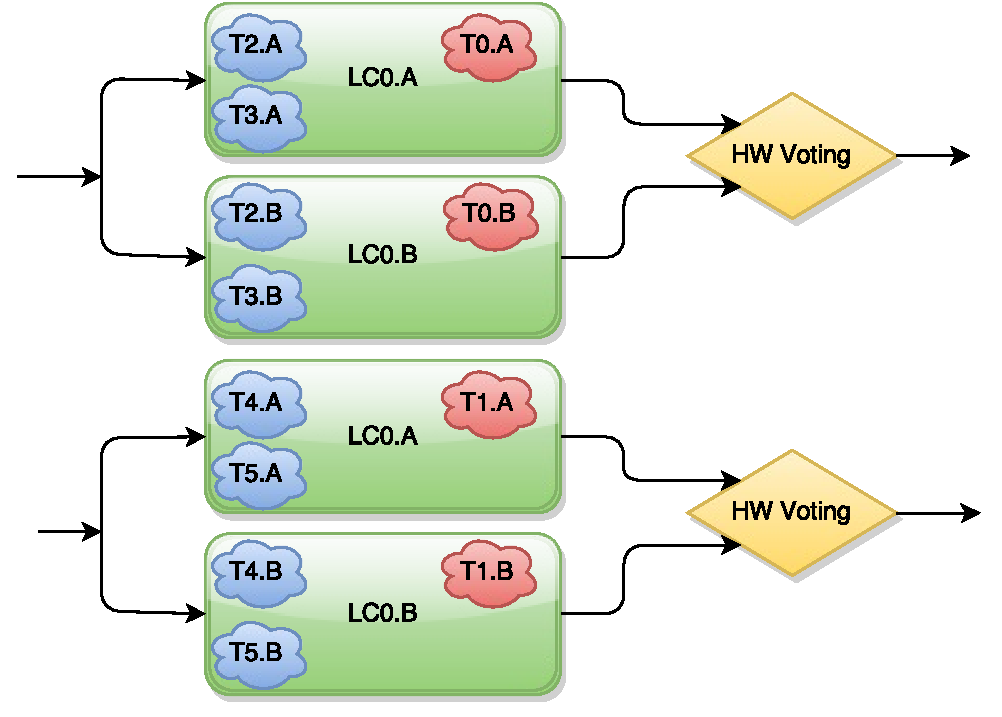
\includegraphics[width=0.42\textwidth]{lockstep.pdf}
}%
\hfill
\subcaptionbox[]{On-demand redundancy \label{f:odr}}[0.45\textwidth]
{
    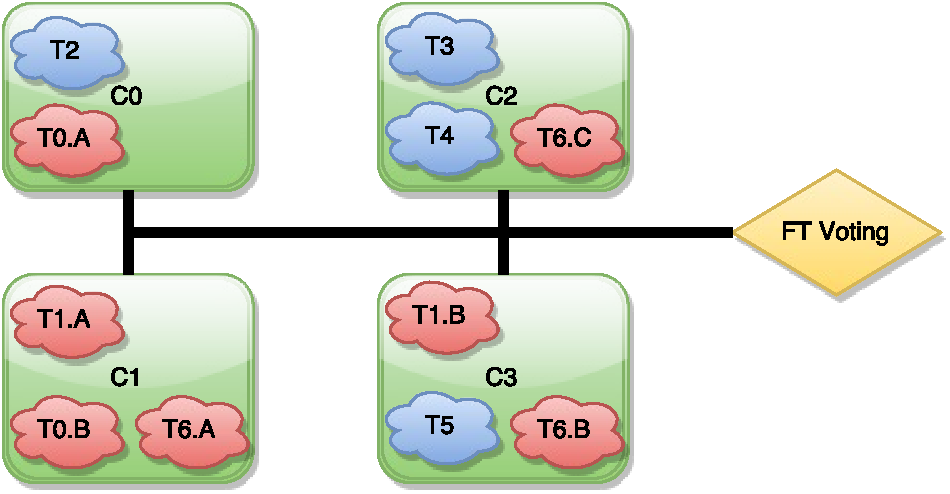
\includegraphics[width=0.42\textwidth]{odr.pdf}
}%
\caption{Different architectures for multicore fault-tolerant systems.}
\label{f:ft-arch}
\end{figure}


\subsection{Fingerprinting with Nios Cores}
\label{s:nios}
	The target architecture is shown in Figure~\ref{f:platform-arch}. 
	A working FPGA prototype has been implemented with Nios II cores in previous work~\cite{ugthesis}. 
	The platform provides a mix of hardened cores and unreliable processing cores. 
	The goal of the platform is to explore the intersection of scheduling theory and a real-life implementation of on-demand redundancy. 
	In a real system at least one core would need to be fault tolerant to form a reliable computing base for the rest of the platform because thread level redundancy cannot catch errors in OS kernel code since it is not replicated \cite{dobel2012watches}. 
	The reliable monitor must be present to take more drastic correction measures (e.g. core reboot) in case the kernel itself is corrupted on any core.
	However, our FPGA prototype does not implement any specific fault tolerance mechanisms as we are concerned with higher level software design and resource management problems. 
	It is sufficient for these purpose to assume one of the cores has internal hardware mechanisms that increase its reliability.


\addfigure{0.6}{arch.pdf}{Platform Architecture}{f:platform-arch}

	ODR is implemented using fingerprinting \cite{Smolens:04} to detect errors. 
	The fingerprint hardware (FP) passively monitors bus traffic and generates checksums based on the write address and data.
	The software on each core signals the start, end, and pausing of a task to the FP unit.
	The hardware supports rate-monotonic scheduling, meaning that a fingerprinted task may be paused and a higher priority task can begin fingerprinting without corrupting the previous fingerprint.
	Preemption is supported using modified exception funnels and stacks inside the FP however the implementation details were the subject of previous work \cite{ugthesis} and will not be discussed in this thesis.
	
	The sphere of replication (SoR) or fault containment region (FCR) refers to the notion that faulty data must not be allowed to propagate to main memory or I/O. 
	The fault tolerant core (FTC) maintains the SoR by moving temporary copies of critical data into the local scratchpad memory (SPM) of each processing core using DMA. 
	The processing cores are then notified to begin execution once the data is prepared. 
	The output of redundant tasks are not directly compared.
	Rather, the fingerprints are compared by an additional comparator hardware module and the results are forwarded back to the FTC. 
	When a task is successful, the FTC copies the data from one of the scratchpads back to main memory.
	
	The execution of redundant threads must be completely deterministic to generate identical fingerprints. 
	For instance, the uTLB implements virtual memory to allow the stack starting addresses and data locations must be identical on both copies for all store addresses to match.
% 	This is achieved using a virtual memory scheme using the uTLB.
	%All functions must take the location of global data as arguments in order to have matching stack references for both cores (Simulink provides this option by choosing reusable function interfaces).

\subsection{Fingerprints and Hamming Distance}
\label{s:hd}
	It must be decided when using fingerprinting how much state to compress into a single fingerprint. The larger the message being compressed, the more likely that \emph{aliasing} may occur, where the faulty fingerprint matches the correct fingerprint. 
	When using CRC, which is a modulo division operation, the likelihood of aliasing for a 32 bit divisor (or generator polynomial) converges to $2^{-32}$ \cite{Maxino:09}.
	
	The Hamming distance (HD) is the number of bits which are different between the faulty message and the correct message. 
	Certain 32 bit polynomials guarantee the absence of aliasing up to HDs of 5 or 6 if the message length is kept fairly small (under 32 kbits) \cite{koopman200232}.
	The argument for short fingerprinting intervals includes minimizing detection latency and decreasing the probability of aliasing.

	This implementation uses architectural fingerprinting as opposed to micro-architectural fingerprinting, meaning that the fingerprinting logic has not been integrated into the CPU and does not fingerprint micro-architectural state such as the register file or pipeline registers \cite{jared2007fingerprinting}.
	We also replicate and restore data at the granularity of a single task execution and are only concerned with the worst case timing.
	Only one fingerprint is necessary per task per period because enough resources must be allocated to handle the worst case latency (which occurs when a task fails near the end of its execution). 
		
	Figures~\ref{f:qsort-d} and \ref{f:qsort} show the average hamming distance (HD) and cumulative HD respectively for the qsort benchmark from the MiBench suite~\cite{guthaus2001mibench}. 
	The results were previously compiled using one and two bit fault injection on an instruction accurate simulation of the PowerPC architecture \cite{georgi}.
	The figures show that the majority of errors with HD less than 10 bits are 1 or 2 bit errors and that the majority of errors result in HDs over 100. 
	We argue that aliasing should not be considered a critical design point since register errors either tend not to propagate or propagate well past the point where lower block sizes can decrease the likelihood of aliasing \cite{Maxino:09}.
	
	
	
\begin{figure}
% \captionsetup[subfigure]{}
\centering
\subcaptionbox{Average HD frequency \label{f:qsort-d}}[0.45\textwidth]
{	
    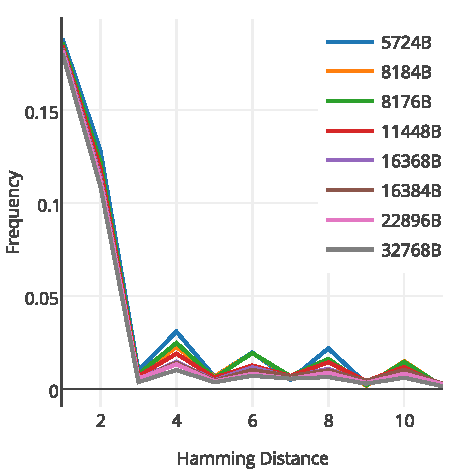
\includegraphics[width=0.45\textwidth]{qsort_d.pdf}
}%
\hfill
\subcaptionbox[]{Cumulative HD frequency \label{f:qsort}}[0.45\textwidth]
{
    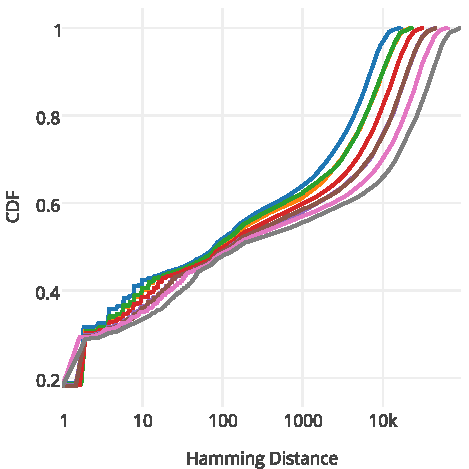
\includegraphics[width=0.45\textwidth]{qsort_nolegend.pdf}
}%
\caption{Fault injection results for qsort on PowerPC architecture}
\label{f:ft-arch}
\end{figure}

\section{Virtual Platform Model}
\label{s:ovp}
	This thesis is primarily concerned with the design and automatic generation of mixed-criticality software that runs on the proposed architecture. 
	All development, validation, and testing is done on a virtual model of the platform using Imperas simulation tools \cite{imperas} built on the Open Virtual Platform (OVP) instruction accurate simulation environment \cite{ovp}. 
	The purpose of developing on the virtual platform is to eventually validate the system on the FPGA implementation, however, software
	calibration on the FPGA is beyond the scope of this thesis.

\section{Simulink and Code Generation}
\label{s:simulink}
	Simulink is a dataflow language used to generate system models and control algorithms which provides the ability to export control algorithms as C code \cite{simulink}. 
	Simulink does not currently support multicore target platforms or fault tolerance. 
	The current state of the embedded runtime environment and assumptions made in the schedulability analysis places some severe limitations on the Simulink generated code supported by the framework presented in this thesis, namely:
\begin{itemize}
  \item The stack and heap requirements of any function cannot exceed 4kB (note that this limit could be increased but that \emph{some} hard limit must exist).
  \item There is no dataflow between tasks.
  \item Code is not generated to send results off-chip (e.g. sending results to actuators via IO).
\end{itemize}




% Chapter Template

\chapter{System Architecture} % Main chapter title

\label{c:tool-arch} % Change X to a consecutive number; for referencing this chapter elsewhere, use \ref{ChapterX}

%----------------------------------------------------------------------------------------
%	SECTION 1
%----------------------------------------------------------------------------------------
	Figure~\ref{f:tool-arch} depicts the code generation and analysis framework. 
	The three main components contributed by this project are the profiling tool, the code generation tool, and the mapping and scheduling tool. 
	Simulink is used to generate the control algorithm C code and the Nios Software Build Tools (SBT) are used to generate and customize board support packages (BSPs) for each core. 
	The BSP contains the Nios Hardware Abstraction Layer (HAL) (the minimal bare-metal drivers provided by Altera), the uC-OS II real-time operating system (RTOS), and the custom drivers required for fingerprinting and thread replication. 

\addfigure{0.59}{toolarch1.pdf}{Tool architecture}{f:tool-arch}
 
	The user provides a configuration file that contains information about the application such as timing requirements for each task in the system. 
	The user may supply their own profiling results or task mappings in the configuration file (if they would like to use an externally derived estimates or if they want to skip the profiling stage after it has already run once). 
	A sample configuration file is provided in Appendix~\ref{A:ConfigFile}. 
	While future work may allow the user to specify a custom hardware configuration, the tool is currently limited to two processing cores and one FTC. 


	The code generation tool (CG) first parses the configuration file and determines if profiling is required. 
	It then generates the necessary inputs for the profiling tool and collects the results (which can include maximum stack depth and worst case execution time). 
	The code generation tool then takes the provided or generated profiling information and forwards it to the Mapping and Scheduling (MS) tool. 
	The MS tool returns an optimal schedule and mapping for the task set. 
	Finally a main file is generated for each core that configures all threads and replication related services as well as scripts to configure the BSP given the mapping. 	The three sets of source files are packaged and scripts are generated to compile the system.
% Chapter Template

\chapter{Software Implementation} % Main chapter title

\label{c:soft-impl} % Change X to a consecutive number; for referencing this chapter elsewhere, use \ref{ChapterX}

%----------------------------------------------------------------------------------------
%	SECTION 1
%----------------------------------------------------------------------------------------
	This chapter will review the semantics of the fingerprint based multicore architecture in Figure~\ref{f:platform-arch}. 
	The implementation details will then be provided for the embedded C code templates. 
	The chapter starts with an overview of the main interactions between the system level components. 
	Each interaction will then be decomposed until the low level behaviour of is exposed. While hardware exists to support TMR, only DMR code generation has currently been implemented at this time. 
	As a general comment on notation, sequence diagrams will be used to depict interactions between physical components in the system. They do not in any way represent an object oriented software implementation. 


\section{System Level Control Flow}
		
	Figure~\ref{f:correct-op} shows the system level control flow for a correct execution of a DMR replicated task.
	The main components in the system that interact in order to implement ODR are the monitor core (FTC), the processing core, the fingerprint (FP) unit, and the comparator. 
	The following interactions when distributed redundant copies of critical tasks are correctly executed in the system. 
	First the monitor configures the comparator. 
	Then the monitor prepares and sends the data and stack to the scratchpads (SPM) of both processing cores. 
	The monitor then notifies the cores to begin execution of the critical task. 
	Each core notifies its FP unit that a critical task is beginning. 
	The FP units then notify the comparator. 
	The FP units send the checksum to the comparator when a task is complete. 
	When all checksums are received the comparator notifies the monitor of the result. 
	If the execution is correct the monitor then copies back one of the correct scratchpad contents. 

\addfigure{0.6}{imp-correct.pdf}{The main sequence of operations in correct execution of a distributed task on the platform}{f:correct-op}


\section{Memory Achitecture}

	The memory architecture in Figure~\ref{f:mem-part} contains several specialized modules and regions of access to enforce fault containment and deterministic execution in redundant threads. 
	Each core has an MPU to enforce memory protection and uTLB for virtual memory management. 
	As previously mentioned, each core executes on copies of data in the SPM while the original copy remains unaltered in main memory. 
	The MPU is used to ensure that the cores do not access the original copy of the data. 
	In a future implementation, a centralized MPU managed strictly by the monitor would be more dependable. 
	The current MPU is contained in the closed-source Nios code and cannot be modified or extended. 
\addfigure{0.6}{mem-part.pdf}{Memory partition of local and global data space.}{f:mem-part}

% \addfigure{0.6}{sor.pdf}{The memory architecture and the sphere of replication.}{f:sor}
	The shared memory is a region of fast on-chip memory used by the monitor and processing cores to communicate using a simple protocol of fixed message types. 
	All data in shared memory is write only for only one core to simplify concurrent data accesses. 
	The monitor core is responsible for initializing the shared data. % (see Section~\ref{s:inter-core}). 

The physical address space is partitioned in order to support a simple virtual memory scheme. The scratchpad of each core has the same local address. The monitor software running on the FTC sends commands to the local DMA of each core when copying data from main memory to the scratchpads. Each DMA is only connected to one local scratchpad. There is no ambiguity as each DMA command port has a unique address in the global space. 

\subsection{Virtual Memory Management}

Fingerprinting requires the address and data to match for all store instructions which in turn requires that the stack pointer be identical on both cores throughout the execution of the task. The uTLB translates the virtual address into the physical address and is programmed by each core according to runtime information provided by the monitor. Deterministic behaviour is guaranteed by fingerprinting the virtual address and ensuring that both cores use the same virtual address. 

The virtual memory management divides each scratchpad into bins according to the page size used by the uTLB. The uTLB page size is programmable at hardware compiled time and is currently set to 4kB. A 16kB scrachpad, for example, contains four bins.  The linker script for each core is updated to reserve one page in main memory for the global data (currently one 4kB page is reserved for \emph{all} global data of fingerprinted tasks rather than on a per-task basis) and one for the stack of each task. The stack size of each task is known statically using profiling information and adding an offset to account for the overhead of context switching and interrupt handling. The virtual address for each stack is assigned statically at design time. The physical address may change at runtime. The virtual addresses of all stacks point to an unused section of the address space.

The linker script exerpt in Listing~\ref{l:virt-mem-link} shows the main memory region of a core has been shortened by 8kB and two 4kB regions called \texttt{stack\_bin\_x} have been added. Listing~\ref{l:virt-mem-init} shows a condensed version of the relevant startup procedure. First, the stack is declared statically and assigned to the stack bin (line 1). The virtual address for the stack is then set up using the uTLB (liens 4-9). Finally, when creating the task (line 11), the virtual address is used. All references by the RTOS to the stack of this function will use the virtual address. When the monitor signals that the core should begin execution, the interrupt handler will retrieve the runtime information from shared memory and update the memory tables before signalling that the task is ready (Listing~\ref{l:cpu-irq}).


\includecode{virt-mem-link.c}{l:virt-mem-link}{Linker configuration for aligned stack pages}{C}
\includecode{virt-mem-init.c}{l:virt-mem-init}{Starting up system with virtual memory}{C}
\includecode{cpu-irq.c}{l:cpu-irq}{Handling an interrupt from the monitor to start task execution}{C}
The RTOS kernel has also been modified to support virtual memory management during context switching. Translation is only enabled for the active task in order to reduce possible sources of error. A simple interface allows memory management to be handled by requesting translation for a task based on its fixed priority number. The context switch code does not check if translation is necessary or if the table has been changed. The memory management interface is naively called during context switch and the memory management internally looks up the task information and updates the uTLB if necessary.

\SetKwIF{Upon}{}{}{Upon}{do}{}{}{end}
\begin{algorithm}
\DontPrintSemicolon
	\Upon{Start task $T_i$}{
		
	}
	\Upon{Enter context switch}{
	
	}
	\Upon{Exit context switch}{
		
	}
	\caption{Memory management procedure during context switch.}
	\label{a:mem-manager}
\end{algorithm}




\subsection{Memory Protection}

Each core has its own operating system and must initialize its stack when creating the new task using the built-in RTOS functions. Once complete, the MPU is enabled before the RTOS starts executing tasks. The MPU catches null pointers, as well as writes to the memory space of other cores or its own critical memory space. This provides some added protection against faults in the non-replicated sections once startup has successfully completed.



% The page size of the uTLB is programmable at hardware compile time and is set to 4kB. The stack pointer must match for the entire function for execution fingerprints to match. So long as the address data


\section{Running Critical Tasks on Processing Cores}

Each critical task is assumed to be called from a single function that takes all global data (including persistent state) as arguments. Listing~\ref{l:crit-task-wrapper} shows a simplified example wrapper (the setting of some global RTOS flags has been omitted). As in any periodic task in a C based RTOS, the function consists of an infinite loop and waits on a semaphore to begin each loop iteration. First, the runtime monitor which measures execution time is notified that the task is starting a new iteration. Then the core resets all of its callee saved registers to 0. This is required for deterministic execution because the contents of callee saved registers are history dependent and may spill onto the stack. 

\includecode{crit-task-wrapper.c}{l:crit-task-wrapper}{Example wrapper function for critical task}{C}

The Nios II architecture includes a global pointer similar to MIPS. Both cores must execute the same critical code since the return addresses will be pushed onto the stack and must match in order for fingerprints to match. The Nios compiler does not guarantee that compiled code does not use the global pointer (the option is specified but unimplemented). However, shared code using Matlabs reusable function option should not generate global pointer references as there are no direct references to static objects. It is possible to temporarily change the global pointer of one core to match anothers as discussed in prior work \cite{ugthesis}.


\subsection{Runtime Monitor}

AMC response time analysis assumes that some runtime monitoring facilities exist to catch when a task exceeds its $C(LO)$ (Section~\ref{}). The runtime monitor maintains a an execution time counter for each execution of all tasks on every core and is responsible for the mode change in case of an overrun. Only the simple two mode behaviour has been implemented and all LO criticality tasks are dropped at the mode change. Reverse mode changes (restarting the LO tasks) has also been omitted.

The runtime monitor must be notified at the beginning and end of each iteration for each task (shown in Listing~\ref{l:crit-task-wrapper} lines 9 and 23). The RTOS kernel must also be modified to update the runtime monitor tables when a context switch occurs. The runtime monitors uses a dedicated timer rather than rely on the OS software clock to improve precision.

\SetKwIF{Upon}{}{}{Upon}{do}{}{}{end}
\begin{algorithm}
\DontPrintSemicolon
	\Upon{Start task $T_i$}{
		Put $T_i$ in table\;
		Mark $T_i$ as running\;
		Reset $T_i$ counter\;
		Reset the timer\;
	}
	\Upon{End task $T_i$}{
		Mark $T_i$ as not running\;
	}
	\Upon{Pause task $T_i$}{
		\If{$T_i$ in table}{
			Add timer value to $T_i$\;
		}
	}
	\Upon{Unpause task $T_i$}{
		Reset the timer\;
	}
	\Upon{System clock interrupt (every ms)}{
		\For{Running task $T_i$}{
			Add timer value to $T_i$\;
			Reset the timer\;
			\If{C >= C(LO)}{
				Drop all LO tasks\;
			}
		}
	}
	\caption{Runtime monitoring of execution time.}
	\label{a:run-mon}
\end{algorithm}
 


% 
% \begin{table}[h]
% \caption{Address Space Partition}
% \centering
% 
% 	\begin{tabular}{@{}ll@{}}
% 	\toprule
% 	Local Peripherals &0x8000000-0x8FFFFFF 	 \\
% 	Scratchpad &0x8420000-0x8427FFF 			 \\
% 	Shared Memory &0x2500000-0x25003FF		\\
% 	Main Memory &0x0000000-0x0095FFF		\\
% 	\end{tabular}
% 
% \label{t:virt-mem}
% \end{table}
	



% what is shared memory? What goes there? how is it used ?
% 
% What is the scratchpad address ?
% 
% what is the distribution of addresses local vs. global ?
% 
% what is the memory virtualization strategy ?


\section{Monitor}

The monitor tasks must run on the FTC. They consist of:
\begin{itemize}
  \item setting up task parameters and initializing all critical task models
%   \item managing dataflow between tasks
  \item intercore task communication
  \item retrieving valid data when critical tasks execute correctly on other resources
  \item restarting tasks in the case of a transient fault
  \item managing the global data space
  \item organizing coordinated virtual memory management and memory protection between cores to achieve correct fingerprinting
\end{itemize}

\subsection{Initializing Data Structures}

The code generation stage assumes that all task computations are encapsulated in functions which take as parameters pointers to any global data used in the computation (no direct reference to global data).


\subsection{Inter-Core Communication}
\label{s:inter-core}
	The contents of the \texttt{SharedMemorySymbolTable} and \texttt{CriticalFunctionData} in Listings~\ref{l:shared-mem-init} are given by Tables \ref{t:stab} and \ref{t:crit-data}, respectively.
	
	% 	space using two data structures: the \texttt{SharedMemorySymbolTable} and \texttt{CriticalFunctionData}
% 
% \includecode{shared-mem-init.c}{l:shared-mem-init}{Shared memory data structures for inter-core communication.}{C}

	
\begin{table}[h]
\caption{Example Task Set}
\centering
	\begin{tabular}{@{}lcccc@{}}
	\toprule
	& $C(LO)$ & $C(HI)$ & T=D & L 	 \\
	\bottomrule
	$\tau_1$ & 3 & 4 & 12 & HI  \\
	$\tau_2$ & 4 & - & 12 & LO  \\
	$\tau_3$ & 4 & - & 12 & LO  \\
	$\tau_4$ & 1 & - & 12 & LO  \\
	\end{tabular}

\label{t:stab}
\end{table}
	

\begin{table}[h]
\caption{Example Task Set}
\centering

	\begin{tabular}{@{}lcccc@{}}
	\toprule
	& $C(LO)$ & $C(HI)$ & T=D & L 	 \\
	\bottomrule
	$\tau_1$ & 3 & 4 & 12 & HI  \\
	$\tau_2$ & 4 & - & 12 & LO  \\
	$\tau_3$ & 4 & - & 12 & LO  \\
	$\tau_4$ & 1 & - & 12 & LO  \\
	\end{tabular}

\label{t:crit-data}
\end{table}
	
	
	
Pointers must also be updated when transferring data to the scratchpads if they are relative to the start address\ldots
\todojc{generate example with functions that use state}


\begin{lstlisting}
/********************************************
 * Pointer relocation functions
 ********************************************/
void RadarTrackerUpdatePointers(INT32U baseAddress, RT_MODEL_RadarTracker_T *RadarTracker_M){
	RadarTracker_M->ModelData.dwork = (DW_RadarTracker_T *)(baseAddress + sizeof(RadarTrackerStruct));
}
\end{lstlisting}

	
	

\subsection{Scratchpad Management}
\subsection{Restarting Tasks and Cores}
\subsection{Fingerprint Management}





% Chapter Template

\chapter{Binary Code Profiling} % Main chapter title

\label{c:prof} % Change X to a consecutive number; for referencing this chapter elsewhere, use \ref{ChapterX}

%----------------------------------------------------------------------------------------
%	SECTION 1
%----------------------------------------------------------------------------------------
\section{IPET Analysis}
The WCET for a function is calculated using implicit path enumeration technique (IPET) \cite{li1995performance}. IPET is a method of pessimistically determining the WCET of a
program without actually identifying the worst-case path. The first step is to convert the CFG into an integer linear program (ILP) and the second step is to determine the cost of each basic block using microarchitectural modelling and/or dataflow analysis. 

The goal of the ILP is to maximize the objective function:

\begin{equation}
\sum_{i=1}^{N}c_ix_i
\end{equation}

where:

\begin{itemize}
  \item $N$: Number of basic blocks
  \item $c_i$: Execution time of block $i$
  \item $x_i$: frequency of block $i$
\end{itemize}

The CFG is transformed into a set of linear constraints by noting that the number of times a basic block is entered must equal the number of times it is exited. Each edge in the CFG is assigned a variable $e_i$. The entry edge into the root basic block has the constraint $e_0 = 1$. For all other edges, constraints are extracted based on the observation that for each basic block: $\sum e_{in} - \sum e_{out} = 0$. For example, in Figure~\ref{f:bbedges}: $e_0+e_1+e_2-e_3=0$.

\begin{figure}[h]
\centering
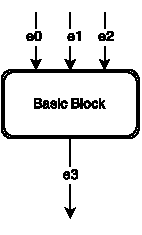
\includegraphics[scale=1]{bbedges.pdf}
\caption{Sum of the edges into the basic block must equal the sum of the edges out: $\sum e_{in} - \sum e_{out} = 0$.} 
\label{f:bbedges}
\end{figure}


% Loops require an additional constraint on the maximum number of times the loop can can run. Therefore for each loop $\sum e_{in} \leq m$ where $m$ is the maximum number of iterations. In Figure~\ref{f:loopedges}, taking $m=10$ gives: $e_0 + e_1 + e_2 + e_4 \leq 10$. Functions calls are not explicitly represented in the constraint system. Each function is analyzed independently and then the final execution time of a basic block $i$ that calls function $f$ is defined as: 
%   $(c_i+WCET(f))x_i$. Recursive function calls are not supported but are also generally not used in real-time systems.


Loops require an additional constraint on the maximum number of iterations. Therefore for each loop $\sum e_{in} - \sum \mathrm{maxIter}*e_{fl} \le 0$, where $\mathrm{maxIter}$ is the maximum number of iterations for the loop and $e_{fl}$ are the non-backwards edges into the loop (i.e. those that can only execute once per single round of loop iterations).


\begin{figure}[h]
\centering
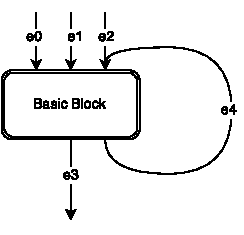
\includegraphics[scale=1]{loopedges.pdf}
\caption{An additional constraint is required for loops: $\sum e_{in} \leq m$.} 
\label{f:loopedges}
\end{figure}


Function calls are handled quite simply. The entry-point to the top-level function simply equals 1. For all other functions, the entry-point equals the sum of all the edges leaving basic blocks that call that function. In Figure~\ref{f:function-ipet}, the result is: $e_2+e_3-e_4 = 0$.

\begin{figure}[h]
\centering
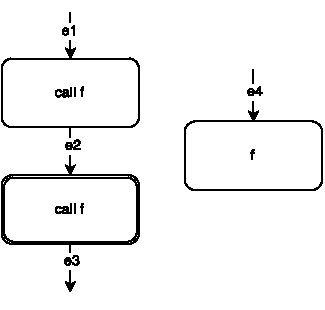
\includegraphics[scale=1]{function-ipet.pdf}
\caption{The sum edges leaving function call blocks is equal to the edge entering that function's root block.} 
\label{f:function-ipet}
\end{figure}
 


\section{Solution Strategy and Implementation}

The pre-existing IR is a basic control flow graph (CFG) constructed from the assembly code. The structure of the IR and tools is shown in Figure~\ref{f:class}. Basic blocks have been identified and the instruction types have been roughly categorized (e.g. branch, binary operation). However, the operation and operands are still in unparsed string form. Before loop analysis can be done, several steps must be taken to create a more meaningful IR for the code within basic blocks.

\addfigure{0.55}{class.pdf}{Class diagram of profiling tool}{f:class}

\addfigure{0.6}{stages.pdf}{Stages of loop analysis}{f:stages}
Building the new IR requires several stages, shown in Figure~\ref{f:stages}. The goal of these analyses is to transform the representation of the program from a list of \texttt{Code} objects into a list of available expressions at each program point, represented as trees with the \texttt{Expression} class. Furthermore, static single assignment (SSA) is used to ensure that the correct version of each variable is being referenced in the loop analysis. Not much will be said about the conversion to SSA form except that it follows the technique found in Appel~\cite{andrew2002modern}. A sample input and output are shown in Listing~\ref{l:ssa-example}. One detail worth mentioning is that function calls cause an increment to the counter of the return registers $r_2$ and $r_3$.


\begin{figure}[h]
\captionsetup{type=lstlisting}
\caption{Example of SSA renaming output}
\begin{sublstlisting}[t]{0.47\linewidth}
\caption{Original Code}
\lstinputlisting[captionpos=t,language=C]{code/ssa.c}
\end{sublstlisting} \hfill
\begin{sublstlisting}[t]{0.47\linewidth}
\caption{Renamed Code}
\lstinputlisting[captionpos=t,language=C]{code/ssa.s}
\end{sublstlisting}
\label{l:ssa-example}
\end{figure}




\subsection{Reaching Expression Analysis}

The reaching expression analysis combines elements of reaching defintion analysis, constant propagation and copy propagation. This analysis, like the normal reaching definition analysis, is a \textit{may} analysis. The use of SSA form simplifies the analysis compared to previous iterations because the $\phi$ function eliminates the need for explicit representation of undefined paths (this will be discussed in more detail later).

\begin{enumerate}
  \item The analysis approximates lists of expressions that may be available on the stack or in registers.
  \item At a program point $p$, we would like to know the expressions that \textit{may} be stored on the stack or in registers.  We would also like to substitute older expressions into newer expressions as they are generated at each $p$ during the analysis if the substitution is \textit{unambiguous} (i.e. if only one definition is reaching).
  \item This is a forwards analysis.
  \item The merge operation is a simple union. 
  \item In general, registers and frame offsets will be considered temporary variables and the entire frame offset (e.g. ``-8(fp)'') will be considered an identifier. The frame pointer can safely be considered a constant value for intraprocedural analysis as it is only modified in the prologue and epilogue.
   
  \textbf{loads}: $out(S) = (in(S) - kill(S)) \cap gen(S)$ where the kill set is any previous expression stored in the destination register and the generated value is either the identifier of the load source or the expression that was stored there if it was known. 
  
  \textbf{moves}: same as load.
  
  \textbf{stores}: $out(S) = (in(S) - kill(S)) \cap gen(S)$ where the kill set is any previous expression stored in the destination address and the generated value is either the identifier of the source register or the expression that was stored there if it was known.
  
  \textbf{binary operators}: $out(S) = (in(S) - kill(S)) \cap gen(S)$ where the kill set is any previous expression stored in the destination register and the generated expression corresponds to the condition of the instruction.
  
  \textbf{conditional branches}: The expression evaluated by conditional branches are useful state to propagate for the loop analysis but is not stored on the stack or in a register. The expression is placed in the out set at a key corresponding to the instruction address.
  
  \textbf{$\phi$ function}: The merge operation combines sets of expressions from different branches. The $\phi$ function explicitly handles the merges of different versions of the same variable. For example $\phi(a_3) \leftarrow a_2,a_1$ generates the set $\{a_3, \{in(a_2) \cup in(a_1)\}\}$. The $\phi$ function kills the sets for $a_2$ or $a_1$.
  
  All other expressions have no effect at the current time. Support for more statement types will be added as necessary. Function calls do not currently kill the values of return registers however they do increment the counter of the return registers in the variable renaming stage. The flow contains a few extra terms due to this limitation.
  
  \item As this is a \textit{may} analysis, $in(start)=\{\}$ and $in(s)=\{\}$. 
\end{enumerate}

An exerpt from the analysis output is shown in Listing~\ref{l:reachexp}. The example shows how expressions are constructed and how known old values of variables are immediately folded into newer ones. The $\phi$ function merges the expressions from the previous definitions into the new one and kills the old references. It is also possible to maintain a symbol table of definitions. The definition of a variable can be unambiguously retrieved since there is only one. Definitions can be conveniently retrieved for variables that have already beek killed in the flow-set for the current line of code when attempting to simplify expressions later on in the loop analysis.

\begin{lstlisting}[caption={Example reaching expression analysis},label=l:reachexp,captionpos=t]
Basic block start address: 10e0
@!Address: 10e0; instruction: movhi; operands: r3_1,0@!
in: {}
out: {r3_1=[(0) << (16)]}
-------------------------------
@!Address: 10e4; instruction: addi; operands: r3_2,r3_1,9248@!
in: {r3_1=[(0) << (16)]}
out: {r3_2=[((0) << (16)) + (9248)], r3_1=[(0) << (16)]}
-------------------------------
@!Address: 10e8; instruction: mov; operands: r2_1,zero@!
in: {r3_2=[((0) << (16)) + (9248)], r3_1=[(0) << (16)]}
out: {r3_2=[((0) << (16)) + (9248)], r2_1=[0], r3_1=[(0) << (16)]}
-------------------------------
@!Address: 10ec; instruction: movi; operands: r4_1,300@!
in: {r3_2=[((0) << (16)) + (9248)], r2_1=[0], r3_1=[(0) << (16)]}
out: {r3_2=[((0) << (16)) + (9248)], r2_1=[0], r3_1=[(0) << (16)], r4_1=[300]}
-------------------------------
****************************************************
Basic block start address: 10f0
@!Address: 10f0; instruction: phi; operands: r3_2,r3_4 -> r3_3@!
in: {r3_3=[], r3_2=[((0) << (16)) + (9248)], r3_4=[(r3_3) + (24), (((0) << (16)) + (9248)) + (24)], ...}
out: {r3_3=[((0) << (16)) + (9248), (r3_3) + (24), (((0) << (16)) + (9248)) + (24)], ...}

\end{lstlisting} 

\section{Loop Analysis}

Algorithm~\ref{a:analysis} shows how the loop is characterized. Note that nested loops do not break the condition that only one backwards edge can exist because a backwards edge is defined as going back to the \textit{head} of the loop. 

The maximum number of iterations of a loop $l$, defined as $M(l)$, is given by the following equation:
\begin{equation}
	M(l) = 
	\begin{dcases*}
		\max{\left \lceil \frac{threshold - initial}{increment} \right \rceil}, & $\{<,>\}$ expressions \\
		\max{\left \lceil \frac{threshold - initial + 1}{increment} \right \rceil}, & $\{\leq,\geq\}$ expressions
	\end{dcases*}
	\label{eq:max}
\end{equation}
and subject to the constraints:
\begin{equation}
(\min(th) > \max(init)) \wedge (\min(inc) > 0), \{<,\leq\} \text{expressions} 
\end{equation}
\begin{equation}
(\max(th) < \min(init)) \wedge (\max(inc) < 0), \{>,\geq\} \text{expressions} 
\end{equation}
Zero and infinite iterations throw exceptions for now. All values in all ranges must respect constraints.
		
The maximum or minimum of each range is chosen as appropriate to maximize $M(l)$.	

	
\begin{algorithm}
\KwData{Function f}
\KwResult{Max iteration for each loop in f}
reachingExp = Reaching expression analysis on f\;
\Begin{
	\For{Loop l in f.getLoops()}{
		String iterator; \tcp{Name of induction variable} \
		Range incrValue; \tcp{Range of values for constant increment} \
		Range threshold; \tcp{Range of constant threshold for loop exit} \
		Range initValue; \tcp{Range of constant initial values for induction} \
		BasicBlock $backEdge\leftarrow$getSingleBackwardsEdge(l)\;
		\If{backEdge == null}{
			fail\;		}
		BasicBlock $exitPoint\leftarrow$getSingleExitPoint(l)\;
		\If{exitPoint == null}{
			fail\;
		}
		conditionOut $\leftarrow$ The reaching expressions at $exitPoint$\;
		branchCondition $\leftarrow$ The expression of the branch condition in $conditionOut$\;
		Simplify $branchCondition$\;
		$iterator \leftarrow$ lefmost identifier in $branchCondition$\;
		\tcp{tricky part} \
		Find expressions $thresholdExp$ and $initExp$\;
		$inSet \leftarrow $ merged output of $\phi(iterator)$ without backwards edge\;
		\If{$inSet$ contains non-constant expressions}{
			\If{inSet.size() $>$ 1}{
				fail \tcp{limit one common unkown for now}
			}
			remove common unknown identifier from $thresholdExp$ and $initExp$\;
		}
		determine ranges from expressions\;
		\If{all ranges defined}{
			$l.maxIterations \leftarrow$ getMaxIterations(initValue,threshold,incrValue,branchCondition.type)\;
		}\Else {
			fail\;
		}
	}
}
 
 \caption{Algorithm for loop analysis.}
 \label{a:analysis}
 \end{algorithm}
 
 \begin{algorithm}
 
\SetKwFunction{getRange}{getRange}
  \SetKwProg{Fn}{Function}{}{}
  \Fn{\getRange{expList}}{
	  $Range \leftarrow$ null\;
	  \For{$exp$ in $expList$}{
	  	\If{$exp$ is binary operation}{
	  		$exp \leftarrow$ simplify $exp$
	  	}
	  	\If{$exp$ is constant}{
	  		$value \leftarrow$ $exp.value$\;
	  		\If{$range$ is null}{
	  			$range \leftarrow [value,value]$\;
	  		}\Else{
	  			\If{$value < range.min$}{
	  				$range.min \leftarrow value$\;
	  			}\ElseIf{$value > range.max$}{
	  				$range.max \leftarrow value$\;
	  			}
	  		}
	  	}
	  	\Else{
	  		\Return null\;
	  	}
	  }
	  \Return $range$\;
  }
  \caption{Get range function for loop detection.}
 \end{algorithm}




\subsection{Example}
It may be easier to demonstrate the behaviour of the analysis with an example. Consider the code in Listing~\ref{l:matmul} and corresponding CFG in Figure~\ref{f:matmul}. This function is interesting because there is nested looping, the inner loops use the array address as induction variables in the assembly code, and the number of iterations can be calculated despite the fact that the initial array address is unknown.

The analysis does not examine the loops in any specific order. The middle-level loop beginning at 0x17a4 is first. The branch condition is then identified (line 4). When the branch condition takes this form then the threshold and increment can be easily identified (lines 7 and 8). The initial condition is also found and the maximum iterations is calculated (lines 9 to 14). The second loop is a bit tricker because the initial value and threshold are offset by a constant unkown (lines 23 and 25). This pattern is recognized by the analysis and the unkown term is cancelled out from both expressions (lines 26 to 29).

\subsection{Conditional branches Depending on Induction Variable}
The expressions for conditional branches inside the body of a loop (that are not the backwards or exit edges) may be checked to see if they depend on the induction variable.The maximum number of times the true branch is taken can then be calculated using Equation~\ref{eq:max} with same increment value and updated threshold and initial values that reflect the condition. For example, a conditional branch with expression \texttt{if(i > 75)} contained in a loop \texttt{for(i = 0; i < 100; i++)} will execute a maximum of 24 times using Equation~\ref{eq:max} with an initial value of 76 and threshold of 100.
 
\begin{lstlisting}[caption={Example output for loop analysis on matrix multiplication code.},label={l:matmul-out},captionpos=t]
loop head: 17a4; tail: 17e0; body: 17a4, 17e0, 17bc,
exit point: BB @17e0
backwards edge head: BB @17e0
branch condition: ((r9_3) + (1)) != (128)
simplified lhs: (r9_3) + (1)
iterator: r9_3
increment: [1]
threshold: [128]
merged inSet: [0]
initial value = [0]
thresholdRange = [128,128]
incrementRange = [1,1]
initialRange = [0,0]
maxIterations = 128
//Second loop *************
loop head: 17bc; tail: 17bc; body: 17bc,
exit point: BB @17bc
backwards edge head: BB @17bc
branch condition: ((r2_4) + (4)) != (r8_2)
simplified lhs: (r2_4) + (4)
iterator: r2_4
increment: [4]
threshold: [r8_2]
merged inSet: [(r8_2) + (-512)]
initial value = [[(r8_2) + (-512)]]
Initial value not constant!
Matching unknown in threshold and initial: r8_2
new initial value: [-512]
new threshold: [0]
thresholdRange = [0,0]
incrementRange = [4,4]
initialRange = [-512,-512]
maxIterations = 128
...
\end{lstlisting}


\printCode{matmul}{Example for loop analysis}{l:matmul}
% \includecode{matmul.c}{l:matmul}{Example code for loop analysis}{C}
\addfigure{0.7}{matmul.pdf}{CFG for matrix multiplication example in Listing~\ref{l:matmul}}{f:matmul}


\section{Validation}
\subsection{Static Analysis}
28 micro-benchmarks were used to test the various forms a loop may have (see Appendix~\ref{A:ProfBench}. The benchmarks are fairly representative of the different forms a loop may take. All benchmarks pass that meet the general pattern outlined in this report. Listing~\ref{l:fail} shows one case that does not work when compiling without optimizations. The analysis only considers the behaviour of the variable in the loop condition and fails to recognize that $x$ is in fact behaving as an induction variable and that $k$ depends on $x$. Interestingly, gcc optimizes out the variable $k$ with -O so a more generic analysis of conditional expressions may improve the loop analysis.

\begin{lstlisting}[caption={Indirect test on induction variable fails.},label=l:fail]
int g8 (){

	int k = 1;
	int x = 0;
	while(k == 1){
		if(x == 105){
			k = 0;
		}
		x++;
		a[x] = x;
	}
	return x;
}
\end{lstlisting}

The matrix multiplication example is one of the benchmarks used in the WCET Workshop competition. Listing~\ref{l:inter} shows a useful case from another benchmark that fails without interprocedural analysis. A summary approach could be used to identify that the missing information is a function argument. However, this information is not easily integrated into the ILP formulation (which I've decided not to discuss in this report). Control flow representing infeasible paths is also generally difficult and requires several ILP problems to be generated representing sets of orthogonal constraints in the solution space. Function pointers are another interesting case that require interprocedural analysis.

\begin{lstlisting}[caption={Interprocedural analysis is necessary to analyze programs that call a function which takes the threshold as an argument.},label={l:inter}]
uint8_t fixFilter(uint8_t *f, int size){
  int i;
  int length = 1 << size;
  int sum = 0;
  for(i = 0; i < length; i++){
    sum = sum + f[i];	
  }   
  // divide by length
  sum = sum >> size;
  return sum;
}
\end{lstlisting}

The maximum number of iterations for each loop is checked by the test framework. The total number of instructions generated by the ILP solver is checked against an instruction accurate simulator. 

Infeasible path detection is a third area of interest where interprocedural analysis could also be of value. For example, in Listing~\ref{l:inter}, it is not possible for both \texttt{g()} and texttt{h()} to be executed. The current analysis does not recognize that both conditions cannot be true in the same pass. There is plenty of existing work on infeasible paths and IPET \cite{gustafsson2006automatic,suhendra2006efficient}.


\begin{lstlisting}[caption={Infeasible path analysis is required to further tighten the WCET estimates.},label={l:inter}]
void paths(x){
	if(x > 0){
		g() //expensive function
	}
	//... later on, x not redefined
	if(x < 0){
		h() //another expensive function
	}
}
\end{lstlisting}


The Malarden benchmarks~\cite{gustafsson2010malardalen} as well as PapaBench~\cite{nemer2006papabench} are often used in work on WCET profiling. This tool should be capable of handling these benchmarks largely without annotations once some form of interprocedural analysis and infeasible path detection are in place. It may be necessary to generate several sets of constraints and iterate over several ILP solutions if the flow information becomes too complex 




\subsection{IPET Validation}

The results of the static analysis and annotations where the analysis still fails can be checked against the instruction accurate simulation of the function. The predicted number of instructions matches the prediction exactly when the analysis is sufficiently robust to represent the nuances of the control flow. We are thus confident that the analysis has been properly implemented. However, the real challenge and art comes in determining cycle accurate response times.

There are some limitations on the IPET analysis. First, recursive functions cannot be analyzed. Any handling of recursive functions will require interprocedural analysis with dynamic call graph generation. A second related issue, pointer analysis is required to determine function pointer targets and build full call graphs. 



Library functions, especially software implemented floating point operations, can also be difficult to analyze. They contain many branches to targets stored in registers making it difficult to build a complete CFG (much like the function pointer except the targets may (or may not) be in the same function body). As a result, some measurement based approximations are used for library functions. Currently, only a subset of floating point operations have been analyzed.


Floating point behaviour is approximated by observing the number of times a loop executed in an OVP simulation environment over several thousand random inputs in the range $[-1000,1000]$. The observed worst case number of loop executions is then used to generate constraints when a floating point operation is encountered in a program. The measured number of instructions are not used because in future work it may still be desirable to analyze the entire floating point function using michro-architectural modelling in which case the number of instructions will not be sufficient. Indirect jump destinations are simply ignored. 

Figure~\ref{f:ipetresults} shows the WCET calculated using IPET normalized to the measured execution time (maximum number of instructions observed in OVP) for all four operations. Single-precision is tested without integer multiplication hardware (SP-SW). Double precision is tested with integer multiplication hardware (DP-SW-I) and without (DP-SW). This chart demonstrates that software-based floating point operations are a source of imprecision that is difficult to overcome. Note that there is no guarantee that this is in fact an \emph{over}-estimate because it is not clear that the inputs tested in fact yield the worst case path (although it is likely an over-estimate).

\begin{figure}[h]
\centering
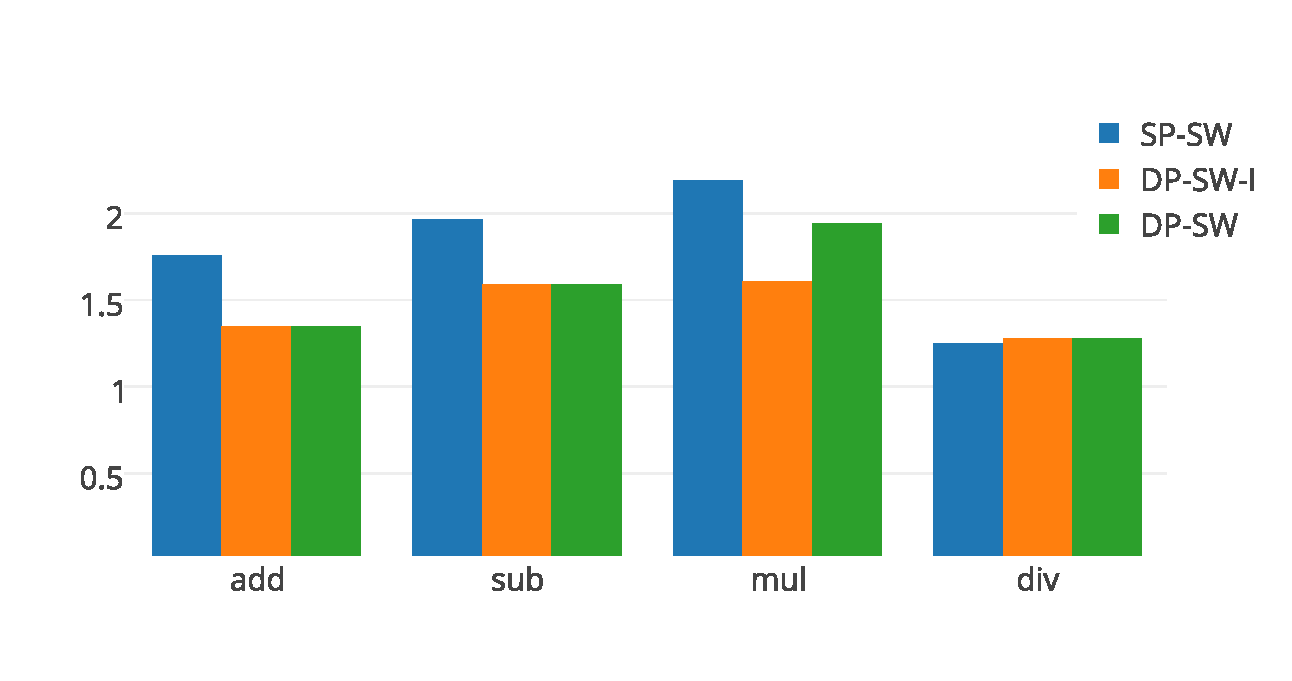
\includegraphics[scale=0.5]{ipetresults.pdf}
\caption{Current IPET analysis over-estimates WCET for software floating point operations compared.}
\label{f:ipetresults}
\end{figure}

This result has motivated the inclusion of FPUs in the cores. The FPU provided by Altera executes single precision operations using the custom instruction interface to the Nios II. Each instruction has a known execution time in clock cycles which eliminates the pessimism in calculating floating point operations. It is possible to force Simulink to generate code using only single precision variables and operations. There is a resulting tradeoff between the accuracy of the WCET estimation, the size of the core (inclusion of an FPU), and limiting calculations to single-precision. The FPU will also remove thousands of instructions from the critical function and reduce the interference due to instruction loads from main memory as well as lower execution time considerably. Future work on michro-architectural modelling may extend this analysis to several physical processors. Existing work on multicore WCET estimation is quite promising~\cite{chattopadhyay2014unified}.

\section{Stack Analysis}
It is possible to start analysis once the parser has built the CFG. Stack analysis is quite straightforward. Each basic block in a function is checked for instructions that increase the stack size. Note that stack instructions should not occur in a loop. If a basic block calls a function, then that function is also checked for stack instructions and then this result is added on to the original calculation. Recursive functions are not supported. Future work could analyze interrupt handlers as well to statically determine the maximum overhead due to interrupt handling.


\section{Library functions}

The object file and archive location of each library function has been determined and made statically available. There are (at least) two potential uses for this data. First, Some library functions may not conform to the patterns described in this Chapter. However, approximations based on runtime profiling could be substituted when library functions are encountered. Second, instruction prefetching into scratchpads requires that the entire call graph is known for the critical function. The library functions must be placed in a contiguous memory page for the simplistic virtual memory system currently implemented. Modifications to the linker script, a shown in Listing~\ref{l:jlib}, require the exact location for each function.

% 
\begin{lstlisting}[caption={Placing library functions in \texttt{.critical} region},label=l:jlib,language=C]
/* Library functions are: __muldf3,__muldi3,__pack_d,__unpack_d,__mulsi3,__lshrdi3,__ashldi3 */
/* To place these functions in a section called critical in linker.x: */
    .critical :
    {
        PROVIDE (_alt_partition_critical_start = ABSOLUTE(.));
        *(.critical .critical.*)

        /* INSERT THE FOLLOWING */

        */libgcc:_mul_df.o
        */libgcc:_unpack_df.o
        */libgcc:_pack_df.o
        */libgcc:_lshrdi3.o
        */libgcc:_ashldi3.o
        */libgcc:_muldi3.o
        */libgcc:lib2-mul.o

        /* END OF INSERTED CODED */

        . = ALIGN(4);

        PROVIDE (_alt_partition_critical_end = ABSOLUTE(.));
    } > processor0_0_scratchpad


\end{lstlisting}



% Chapter Template

\chapter{Mapping and Scheduling} % Main chapter title

\label{c:sched} % Change X to a consecutive number; for referencing this chapter elsewhere, use \ref{ChapterX}

%----------------------------------------------------------------------------------------
%	SECTION 1
%----------------------------------------------------------------------------------------

	The two mode AMC response time analysis for mixed criticality systems was presented in Section~\ref{s:mixedcriticality}. 
	This chapter presents a four mode model that is advantageous for quality of service when both transient faults and execution time overruns are possible in a single lockstep-core mixed criticality fault tolerant system (MCFTS) \cite{albayati2016modes}. 
	A discussion of the four mode analysis and initial single core results on improved quality of service (QoS) will be followed by an extension of the technique to multicore systems and ODR strategies. 
	A DSE mapping algorithm that uses the new analysis will then be presented.

\section{Four Mode MCFTS Model}
\label{s:mcfts}
	AMC response time analysis depends on the notion that safety critical systems must be proven operational under optimistic and pessimistic worst case execution time estimates. 
	A runtime mechanism must be available to monitor the execution time of tasks in the system.
	Some or all LO tasks must be dropped from the system when a any task overruns its optimistic execution time budget.
	In order to accomodate fault tolerance, we extend the analysis to scenarios where a task may also execute more than once in case of failure.
	In this work we assume that the OS kernel does not fail (is perhaps protected through some other strictly software based mechanism that would cause unreasonable delays if applied to the whole program such as \cite{reis2005swift}).
	
	Initial work on AMC assumed that all LO tasks are dropped during a mode change. 
	Current work in MCS aims to reduce the amount of LO criticality tasks that must be dropped through migration in multicore systems \cite{al2015enhanced} and designer specified importance \cite{fleming2014incorporating}. 
	We introduce a four mode model to MCFTS in order to reduce the number of LO tasks that must be dropped in the event that only an execution overrun or transient fault occurs rather than both. 
	We initially consider a lockstep core that is capable of detecting but not correcting errors.
	The RTOS kernel is assumed to remain uncorrupted.
	Under these conditions, a task may be re-executed when an error is detected.
		The four modes intuitively improve QoS because any response time analysis that considers both faults and overruns at the same time will be overly pessimistic in deciding which tasks to drop.
	\addfigure{0.6}{modes.pdf}{The 4 modes of operation in MCFTS analysis.}{f:modes}
\addfigure{0.6}{sched-example.pdf}{Mode change scenarios.}{f:mode-scenarios}
	
	The four modes and their transition conditions are shown in Figure~\ref{f:modes}. 
	Initially, the system is in LO mode. 
	When a transient fault is detected, the system transitions into TF mode. 
	If an execution overrun occurs ($C>C(LO)$), then the system transitions into OV mode. 
	Finally, a transition to HI mode occurs from one of the intermediate mode if the other event occurs before a transition back to LO mode.\footnote{Reverse transitions are usually treated as a separate problem in MCS and is not considered in this thesis. Possible implementation may be found in \cite{bate2015bailout}.}
	
	Three example scenarios are presented in Figure~\ref{f:mode-scenarios} for the task set in Table~\ref{t:example}. 
	In scenario (a), $\tau_1$ exceeds its $C(LO)$ threshold of 3 and the system transitions into OV mode. In scenario (b), $\tau_1$ suffers a transient fault and required re-execution. The system stays in TF mode because none of the re-executions exceed $C(LO)$. In scenario (c), $\tau_1$ first exceeds $C(LO)$ and the system transitions to OV mode. Once in OV mode, an fault occurs and the system transitions into HI mode, presumably dropping even more tasks.
	

	
	
\subsection{Response Time Analysis}
	
	
	\begin{table}[h]
\caption{Example Task Set}
\centering

	\begin{tabular}{@{}lcccc@{}}
	\toprule
	& $C(LO)$ & $C(HI)$ & T=D & L 	 \\
	\bottomrule
	$\tau_1$ & 3 & 4 & 12 & HI  \\
	$\tau_2$ & 4 & - & 12 & LO  \\
	$\tau_3$ & 4 & - & 12 & LO  \\
	$\tau_4$ & 1 & - & 12 & LO  \\
	\end{tabular}

\label{t:example}
\end{table}
	
	%In addition to the LO and HI modes, there is now a transient fault (TF) and overrun (OV) mode. 
	Equations \ref{eq:lomode}-\ref{eq:hiovmode} show the updated four mode response time analysis.
	
	
\begin{equation}
R_i^{(LO)}= C_i(LO)+\sum_{j \in hp(i)}\Big\lceil\frac{R_i^{(LO)}}{T_j}\Big\rceil \cdot C_j(LO)
\label{eq:lomode}
\end{equation}

\begin{equation}\label{eq:ovmode}
\begin{aligned}
R_i^{(OV)} &  = C_i(L_i)+\sum_{j \in hpC(OV,i)}\Big\lceil\frac{R_i^{(OV)}}{T_j}\Big\rceil \cdot C_j(L_j) 
 +\sum_{k \in hp(i)-hpC(OV,i)}\Big\lceil\frac{R_i^{(LO)}}{T_k}\Big\rceil \cdot C_k(LO)
\end{aligned}
\end{equation}
	
	
	The LO mode analysis remains unchanged. Equation~\ref{eq:ovmode} shows the response time for the OV mode. 
	The set of tasks $hpC(L,i)$ is defined as the set of tasks with higher priority than $\tau_i$ that are not dropped in mode $L$. 
	Therefore, in the OV mode, we can see that the jobs that continue to execute are assumed to take the maximum amount of time $C(OV)=C(HI)$ whereas the dropped jobs ($hp(i) - hpC(OV,i)$) only execute during $R_i(LO)$ for up to their $C(LO)$ times.
	
\begin{equation}\label{eq:tfmode}
\begin{aligned}
R_i^{(TF)} & = n_i(TF) \cdot C_i(LO)
+\sum_{j \in hpC(TF,i)}\Big\lceil\frac{R_i^{(TF)}}{T_j}\Big\rceil \cdot n_j(TF) \cdot C_j(LO) \\
&  +\sum_{k \in hp(i)-hpC(TF,i)}\Big\lceil\frac{R_i^{(LO)}}{T_k}\Big\rceil \cdot C_k(LO)
\end{aligned}
\end{equation}

	Equation~\ref{eq:tfmode} shows the response time for TF mode. 
	In the transient fault mode at least one task must re-execute. 
	Each task is assigned a maximum number of executions that it is required to run, $n_i$, in order to meet some threshold in terms of probability of failure (derivation in \cite{albayati2016modes}). 
	In the TF mode, the execution time is still assumed not to exceed the optimistic threshold $C(LO)$. 
	The resulting execution time for task $\tau_i$ is $n_i(TF) \cdot C_i(LO)$ where $n_i$ is the number of re-executions required in the TF mode.\footnote{$n$ depends on $C$, therefore it is possible that $n(TF) \ne n(HI)$ though this is not often the case.}

	Finally, Equations~\ref{eq:hiovmode} and \ref{eq:hitfmode} show the response time analysis for transitions from OV to HI and TF to HI modes, respectively. The set of dropped jobs on the final transition is different for the two modes.





\begin{equation}\label{eq:hiovmode}
\begin{aligned}
R_i^{(HI-OV)} & = n_i(HI) \cdot C_i(L_i) 
  +\sum_{j \in hpC(HI,i)}\Big\lceil\frac{R_i^{(HI-OV)}}{T_j}\Big\rceil \cdot n_j(HI) \cdot C_j(L_j) \\
&  +\sum_{k \in hpC(OV,i)-hpC(HI,i)}\Big\lceil\frac{R_i^{(OV)}}{T_k}\Big\rceil \cdot C_k(LO) \\
& \hspace{1cm}  +\sum_{l \in hp(i)-hpC(OV,i)}\Big\lceil\frac{R_i^{(LO)}}{T_l}\Big\rceil \cdot C_l(LO)
\end{aligned}
\end{equation}

\begin{equation}\label{eq:hitfmode}
\begin{aligned}
R_i^{(HI-TF)} & = n_i(HI) \cdot C_i(L_i)
  +\sum_{j \in hpC(HI,i)}\Big\lceil\frac{R_i^{(HI-TF)}}{T_j}\Big\rceil \cdot n_j(HI) \cdot C_j(L_j) \\
&  +\sum_{k \in hpC(TF,i)-hpC(HI,i)}\Big\lceil\frac{R_i^{(TF)}}{T_k}\Big\rceil \cdot C_k(LO) \\
& \hspace{1cm}  +\sum_{l \in hp(i)-hpC(TF,i)}\Big\lceil\frac{R_i^{(LO)}}{T_l}\Big\rceil \cdot C_l(LO)
\end{aligned}
\end{equation}

\subsection{Reducing Model Pessimism}

	The model is still highly pessimistic as \emph{all} tasks are assumed to re-execute upon a transition into TF mode. 
	This pessimisim is reduced by the introduction of a new parameter $F$, the maximum number of faults expected in an interval $D_{max}$, the largest relative deadline among the tasks in the task set.
	For example, if $\tau_i$ and $\tau_j$ preempt $\tau_k$, then it is obviously beneficial when calculating the response time of $\tau_k$ that \emph{only} $\tau_i$ \emph{or} $\tau_j$ may preempt $\tau_k$ but not both.

	The term $n_i$ in the response time equations for HI and TF modes may be replaced with a new term $1 + f_i$ where $f_i$ is the maximum number of faults that may occur for task $\tau_i$. The updated equation for $R^{(TF)}$ is given by:
	\begin{equation}\label{eq:mode3new}
\begin{aligned}
R_i^{(TF)} & = (1+f_i) \cdot C_i(LO) \\
&  +\sum_{j \in hpC(TF,i)}\Big\lceil\frac{R_i^{(TF)}}{T_j}\Big\rceil \cdot (1+f_j) \cdot C_j(LO) \\
&  +\sum_{k \in hp(i)-hpC(TF,i)}\Big\lceil\frac{R_i^{(LO)}}{T_k}\Big\rceil \cdot C_k(LO)
\end{aligned}
\end{equation}
under the constraints:
\begin{subequations}
%\small
\begin{equation}
0 < f_i \le n_i - 1,  \forall \tau_i
\end{equation}
\begin{equation}
\sum_i{f_i} \le F.
\end{equation}
\end{subequations}

\subsection{Four Mode QoS Results for Single Core}
\label{s:singlecore-results}
	We defined QoS to be the percentage of LO criticality tasks not dropped in any given mode. The QoS for the LO mode is always 1. Random task sets were generated according to the UUnifast algorithm \cite{bini2005measuring} such that LO mode utilization is approximately 80\% on all cores. The ratio $C(HI)/C(LO)$ is determined randomly from the range $[1,2]$ and periods were chosen at random from the set ${10,20,40,50,100,200,400,500,1000}$. For each test, the average of 1000 systems is presented.

\addfigure{0.6}{final-allModesNoF.pdf}{Modes OV and TF achieve better QoS than HI for all utilizations ($F$ not bounded).}{f:util_basic}
\addfigure{0.6}{averageQoS.pdf}{Average improvement over all system utilizations for OV and TF modes compared to HI mode. }{f:avgU}

	Figure~\ref{f:util_basic} shows the QoS of OV and TF modes is improved over the HI mode for all utilizations in systems of 20 tasks (10 HI and 10 LO). LO task QoS is better in the OV and TF modes than in the HI mode. On average, the OV and TF modes outperform the HI mode by 42.9\% and 20.2\% respectively. The improvement increases with the utilization, especially for the OV mode which could be significant in systems where transient faults are less frequent than execution time overruns. Figure~\ref{f:avgU} shows the average improvement of QoS across all utilizations for the TF and OV mode compared to the HI mode.
	
\addfigure{0.6}{final-percentHI.pdf}{Modes OV and TF achieve better QoS than HI for different percentages of HI tasks ($F$ not bounded).}{f:perchi_basic}
	
	Figure~\ref{f:perchi_basic} shows a similar picture, this time holding utilization constant at 80\% while exploring the percentage of HI tasks. The QoS of the HI and TF modes degrade quickly as the percentage of HI tasks increases because none of these tasks can be dropped and the penalty for re-execution becomes very severe.
	 	
\addfigure{0.6}{TFmodeAvgu.pdf}{Performance of TF mode for different $F$}{f:avgUN}
	Figure~\ref{f:avgUN} shows how the $F$ parameter improves QoS for the TF mode ($F=\infty$ is the default). QoS improves by about 15\% compared to the default when only two errors are assumed to occur close enough in time to affect the same mode change.

\section{Extending Response Time Analysis to ODR}

	We will extend the analysis on lockstep (LS) to support three types of ODR. The four scenarios are shown in Figure~\ref{f:ftm}. 
	In (a), LS execution occurs when a node has internal mechanisms for detecting but not correcting errors. 
	An error simply results in a re-execution on that node, as previously discussed. 	
	In (b), dual modular redundancy (DMR) replicates a thread on two cores that cannot detect errors by themselves. 
	The task must be re-executed if the executions do not match according to some external comparison or voting mechanism.
	In (c), triple modular redundancy (TMR) replicates a thread on three cores that cannot detect errors. 
	If an error occurs, the majority answer is taken from the three replicas and no re-execution is required (the system assumes only one replica may fail at a time).
	Finally, in (d), passive replication is similar to TMR but the final replica does not execute if the first two copies return the same result. 


\addfigure{0.55}{ftm.pdf}{The 4 fault tolerance mechanisms supported by the proposed MCFTS analysis}{f:ftm}
	
	Each technique is expressed in the new analysis by three parameters: a task set transformation, mapping constraints, and a re-executiong profile denoted by $N$.
	The task set transformation represents each replica explicitly in the task set. 
	Consider the example task set in Table~\ref{t:transform}. 
	Lockstep does not introduce any replicas to the system and does not require any transformation of the task set. 
	DMR requires one replica to be added to the task set while TMR and PR require two replicas to be added.
	
	Constraints must be added to the problem for the processors $\pi_i$ assigned to $\tau_i$ in order to properly reflect the semantics of the different techniques. 
	The constraints shown in the table ensure that the replicas are not assigned to the same core. 
	These constraints will be useful in the mapping stage.
	
	
\begin{table}
\centering
\caption{Task set transformations}
\label{t:transform}
	\begin{subtable}{0.3\textwidth}
		\caption{Example task set}
		\begin{tabular}{@{}l|cccc@{}}
		\toprule
		& C(LO) & C(HI) & T=D & L 	 \\\bottomrule
		$\tau_1$ & 5 & 10 & 25 & HI  \\
		$\tau_2$ & 5 & - & 20 & LO  \\
		\multicolumn{5}{c}{ } \\
		\multicolumn{5}{c}{ } \\
		\end{tabular}
	\end{subtable} \hspace{2cm}
	\begin{subtable}{0.3\textwidth}
		\caption{DMR transformation}
		\begin{tabular}{@{}l|cccc@{}}
		\toprule
				& C(LO) & C(HI) & T=D & L	 \\\bottomrule
		$\tau_1$ & 5 & 10 & 25 & HI  \\
		$\tau_{1.1}$ & 5 & 10 & 25 & HI  \\
		$\tau_2$ & 5 & - & 20 & LO  \\
		\multicolumn{5}{c}{$\pi_1 \ne \pi_{1.1}$}
		\end{tabular}
	\end{subtable}
	
	\begin{subtable}{0.3\textwidth}
		\caption{TMR transformation}
		\begin{tabular}{@{}l|cccc@{}}
		\toprule
				& C(LO) & C(HI) & T=D & L	 \\\bottomrule
		$\tau_1$ & 5 & 10 & 25 & HI  \\
		$\tau_{1.1}$ & 5 & 10 & 25 & HI  \\
		$\tau_{1.2}$ & 5 & 10 & 25 & HI  \\
		$\tau_2$ & 5 & - & 20 & LO  \\
		\multicolumn{5}{c}{$\pi_1 \ne \pi_{1.1} \ne \pi_{1.2}$}
		\end{tabular}
	\end{subtable} \hspace{2cm}
	\begin{subtable}{0.3\textwidth}
		\caption{PR replication}
		\begin{tabular}{@{}l|cccc@{}}
		\toprule
		& C(LO) & C(HI) & T=D & L	 \\\bottomrule
		$\tau_1$ & 5 & 10 & 25 & HI  \\
		$\tau_{1.1}$ & 5 & 10 & 25 & HI  \\
		$\tau_{1.2}$ & 5 & 10 & 25 & HI  \\
		$\tau_2$ & 5 & - & 20 & LO  \\
		\multicolumn{5}{c}{$\pi_1 \ne \pi_{1.1}$}
		\end{tabular}
	\end{subtable}
\end{table}


	The re-execution variable $n_i$ has been generalized into the vector:
\begin{equation}
	N_i=<n_i(LO),n_i(OV),n_i(TF),n_i(HI)>
\end{equation} 
	The $N$ for each mode is shown in Table~\ref{t:reex} and the updated equation for the OV mode response time are given by the following equations:
	\begin{equation}
\begin{aligned}
R_i^{(OV)} =
\begin{dcases*}
C_i(L_i)\color{red} \color{black}+\sum_{j \in hpC(OV,i)}\Big\lceil\frac{R_i^{(OV)}}{T_j}\Big\rceil \cdot C_j(L_j) \\
\hspace{0.3cm} +\sum_{k \in hp(i)-hpC(OV,i)}\Big\lceil\frac{R_i^{(LO)}}{T_k}\Big\rceil \cdot C_k(LO), &  $n_i(OV)>0$ \\
	0, & $n_i(OV)=0$
\end{dcases*}
   \end{aligned}
\end{equation}
	We note that all techniques have $n(LO)$ and $n(OV)$ values of either 0 or 1. When $n=0$, the task is not executing and the response time is simply 0. The same is true for LO mode.
	
	For example, TMR has $N=<1,1,1,1>$. This means that in all modes, any task using TMR will have $n=1$ which in effect signals that no re-executions are required. For PR, one replica executes one time in all modes and the other only executes in the case of a fault (hence only executes once in TF or HI modes).

	\begin{table}
\caption{Re-execution profiles for the fault tolerance mechanisms}
\label{t:reex}
\centering
	\begin{tabular}{@{}l|c@{}}
	\toprule
	Technique & Profile ($N$) \\
	\bottomrule
	LS & $<1,2,1,2>$ \\
	DMR & $<1,2,1,2>$ \\
	TMR & $<1,1,1,1>$ \\
	PR & $<1,1,1,1>$ and $<0,1,0,1>$ \\
	\end{tabular}
\end{table} 	

\section{Design Space Exploration}

\subsection{Genetic Algorithm}
\begin{figure}[h]
\centering
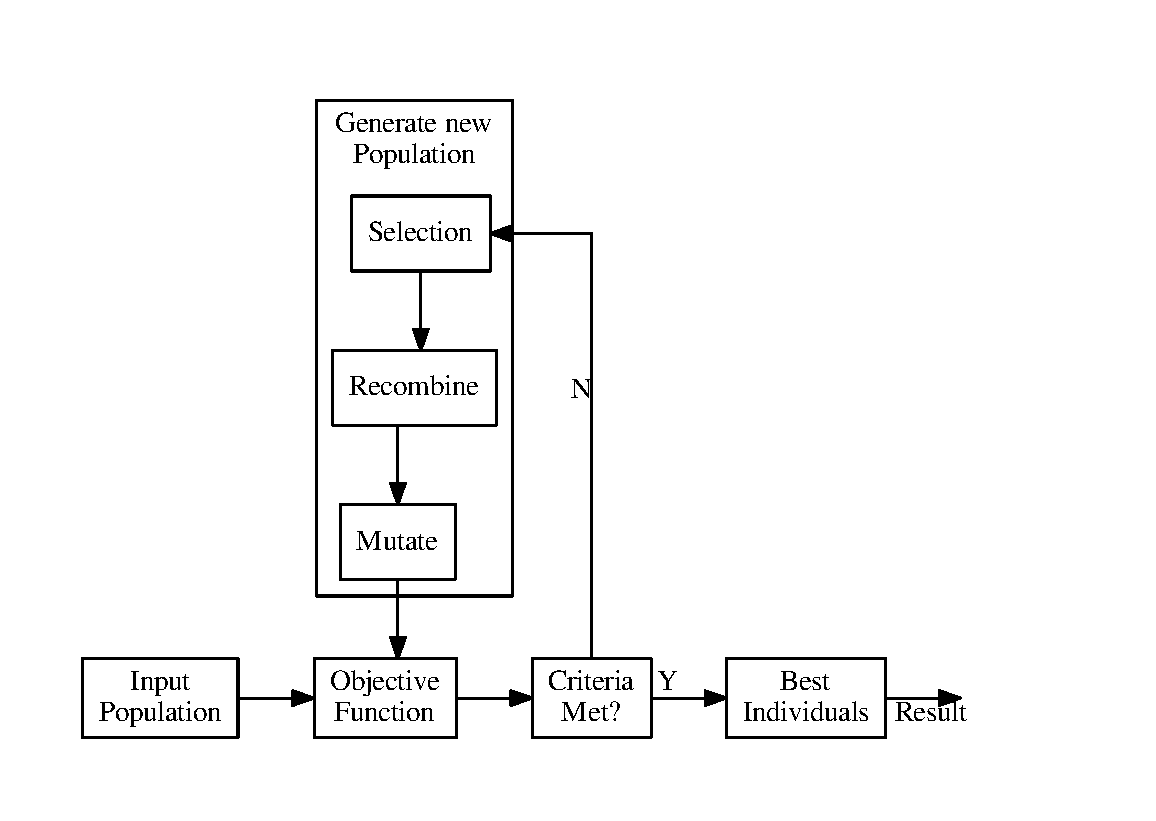
\includegraphics[width=12cm]{ga_ov}
\caption{The basic structure of a genetic algorithm \cite{geatbx}.}
\label{f:ga_ov}
\end{figure}

	Genetic algorithm is an unsupervised exploration technique that attempts to find optimal answers in large problem spaces. 
	Genetic algorithms operate on \emph{chromosomes} which are essentially a vector representation of the problem space.
	An initial population of chromosomes are rated using an \emph{objective} or \emph{fitness} function which determines the quality of each result. 
	If a sufficient answer has been found then the algorithm may quit.
	Otherwise, a new population is generated using selection, recombination and mutation. 
	
	There are many variations on each of these operations. Selection could be as simple as passing on the top $x$ chromosomes and then randomly generating the remainder of the population after each \emph{generation}. 
	Another alternative is tournament selection, where pairs of chromosomes are selected randomly from the population and the higher of the two is passed on to the next generation. 
	Recombination is typically done using the crossover operator which chops two chromosomes at some \emph{gene} location (element index) and swaps the ends.
	Finally mutation randomly modifies a randomly selected gene in a randomly selected chromosome.
	There are many probabilistic parameters that require calibration for each operator as well as the population size and number of generations.
	
	There is not a generally well defined methodology for selecting these parameters. These experiments will evolve a population of size 100 over 30 generations. 80\% of chromosomes are selected from the previous generation using tournament selection. The tournament selection itself passes on the best chromosomes with a probability of 80\%. The crossover rate is 40\% and the mutation rate is 50\%.

\subsection{Two Stage GA}
	The mapping and scheduling algorithm follows the procedure used in \cite{bolchini2013reliability} and \cite{kang2014reliability}. 
	Two stages of genetic algorithms (GA) are used to explore both the techniques used to harden each task and the core assignment for each task and its replicas. 
	The basic flow is shown in Figure~\ref{f:dse}. 
	The GA is implemented using JGAP \cite{jgap}.  
	The Reliability Aware (RA) stage is responsible for mapping a fault tolerance mechanism to each task. 
	The RA stage then generates a chromosome structure for the Mapping and Scheduling (MS) stage. 
	The MS stage attempts to find an allocation for each task onto a core that maximizes the average QoS across all modes in the system using the response time analysis from Section~\ref{s:mcfts}.
	
\addfigure{0.6}{dse.pdf}{Overview of DSE workflow using nested genetic algorithm searches}{f:dse}
	
	The chromosome in the RA stage has one gene for each task and each gene is an integer representing a fault tolerance mechanism being used in the system. 
	For instance, consider a task set with three HI tasks ${\tau_1,\tau_2,\tau_3}$ being mapped onto a platform that supports LS, DMR and TMR - the chromosome would consist of three genes each limited to integers in the range $[0,2]$. 
	
	The RA fitness function (FF) must determine the fitness (QoS) for each configuration of fault tolerance mechanisms. 
	The FF creates a new task set using the transformations in Table~\ref{t:transform} as well as the necessary constraints. 
	The FF then creates a chromosome template for the MS stage based on the transformed task set. 
	Given the number of processors that a task can be mapped to, $n$, it is possible to determine for each FTM a mapping rule that generates a unique configuration from an integer. 
	Each gene in the chromosome is an integer representing a unique allocation for a task and its replicas. 
	It is important that the task and replicas are represented by a single gene or else most chromosomes will result in illegal configurations after mutation and crossover. 
	Table~\ref{t:mschrom} shows the number of configurations for each type of FTM and how to derive a unique allocation as a function of the number of candidate cores ($n$) from a random integer $x < n$. 
	The conversion rule provides an index into an ordered list of the cores. After each core is allocated it is removed from the list.
	
	For example, consider a task and two replicas using TMR in a sytem with 5 processing cores. 
	All three tasks must go on different cores. 
	The number of configurations is $5 \cdot 4 \cdot 3 = 60$. 
	The GA will generate a random integer in the range $[0,59]$ representing a unique mapping of the three tasks onto the system, say 47. 
	The number 47 is converted using the TMR rule to $(47/(4\cdot3),(47\bmod(4\cdot3))/3,47\bmod3) = (3,3,1)$. 
	Suppose the core list is $\{\pi_1,\pi_2,\pi_3,\pi_4,\pi_5\}$. 
	The first copy is allocated to $\pi_3$ and $\pi_3$ is then removed from the list. 
	The next copy is assigned to $\pi_4$ (now at index 3) and the third copy is assigned to $\pi_1$. 
	
	\begin{table}
\caption{Rules for generating unique MS configurations from an integer $x$ for $n$ cores}
\label{t:mschrom}
\centering
	\begin{tabular}{@{}l|cc@{}}
	\toprule
	Technique & Configurations & Conversion Rule \\
	\bottomrule
	none & $n$ & $(x)$\\
	LS & $n$ & $(x)$ \\
	DMR & $n(n-1)$ & $(\frac{x}{x-1},x\bmod{x-1})$ \\
	TMR & $n(n - 1)(n-2)$ & $(\frac{x}{(n - 1)(n - 2)}, \frac{x\bmod ((n-1)*(n-2))}{n-2}, x \bmod (n-2))$ \\
	PR & $n^2 (n-1)$ & $(\frac{x}{n(n - 1)}, \frac{x \bmod (n*(n-1))}{n-1}, x \bmod (n-1))$ \\
	\end{tabular}
\end{table} 	

	A unique MS stage is instantiated for each chromosome in the RA stage population. 
	The MS stage converts the chromosme into a schedule and passes it along to the schedulability analysis. 
	If the system is schedulable then the chromosome is assigned a fitness value equal to the average QoS across all four modes (defined as percentage of LO tasks that have not been dropped).
	If the analysis fails then the chromosome is assigned a fitness value of 0.
	
	
\subsection{Performance Optimization}

	The performance overhead of nesting one lengthy search inside another is problematic. 
	The performance impact was resolved by modifying the RA stage to request a new thread from a pool whenever calling the RA fitness function. 
	Using 20 threads on a 30 core system resulted in significant speedups and makes this a much more practical implementation given sufficient computing resources. 
	We furthermore implement early exiting if a solution is found with perfect QoS or the best QoS has not been improved in four generations.

\subsection{Results}


	Three platforms were tested to verify the mapping: one system (ODR) with four cores using only DMR, the second (LS) with two lockstep cores, and the third (FP) using one lockstep core and two processing cores using DMR. 
	The same task generation algorithm was used as in Section~\ref{s:singlecore-results}. 
	The systems were tested with 100 task sets with between 20 and 40 tasks, half of which were HI, an average utilization of 80\%, and a maximum WCET factor ($C(HI)/C(LO)$) of 3. 
	Note that for the ODR and LS systems, the RA stage could be skipped for efficiency purposes as there is only one available mechanism.

	Any system that is schedulable for one system should be schedulable for all three. 
	They should only differ (possibly) in the QoS of each mode. 
	Furthermore, we expect the QoS of the ODR and FP systems to be higher than that of the LS.  

	Figure~\ref{f:platform-sched} shows the schedulability results for the three platforms. 
	The schedulability of ODR and LS were 69\% and 70\% respectivey. 
	In three cases, the tool failed to find a solution with ODR for a system that passed with LS while only two cases occurred where a LS solution was not found for a system that passed with ODR. 
	The schedulability for the FP platform was 31\% suggesting poor calibration of the GA stages. However, integration with a code generation tool would ideally allow for a very short run time which most recalibrations would significantly extend. 
	Overall, this suggests that the use of genetic algorithms may be a useful starting point but that other semi-random unguided heuristics should also be explored in future work.
	
	Figure~\ref{f:platform-sched} shows the results for average QoS only for task sets successfully scheduled on all three platforms. 
	Here we see that ODR does indeed provide better QoS compared to LS.
	FP provides better QoS in the first three modes compared to LS but not in the HI mode.
	
\addfigure{1}{platform-sched.pdf}{Schedulability results for three different platforms}{f:platform-sched}
\addfigure{1}{platform-qos.pdf}{QoS of the four modes for three different platforms.}{f:platform-qos}


% Chapter Template

\chapter{Code Generation} % Main chapter title
\label{c:code-gen}


%----------------------------------------------------------------------------------------
%	SECTION 1
%----------------------------------------------------------------------------------------
	The code generation framework is designed to automate the porting of Simulink generated control algorithms to the architecture presented in Figure~\ref{f:platform-arch}. 
	The structure of the application being ported follows the assumptions made in the schedulability analysis presented in Chapter~\ref{c:sched}, mainly that tasks are independent and periodic, and that an optimistic and pessimistic WCET have been specified. 
	The hardware and generated code support both DMR with re-execution and TMR for error correction, as well as execution time monitoring. 
	Only a simplified two mode model has been implemented at this time.
	
% 	This chapter begins with a detailed view of the semantics of on-demand redundancy implemented using fingerprinting on the multicore architecture in Figure~\ref{f:platform-arch}. 
% 	The chapter starts with an overview of the main interactions between the system level components, each of which will be discussed in more detail in subsequent sections. 
% 	Finally, the code generation procedure is discussed along with some examples of generated systems.
	
	
	Error detection is implemented using fingerprinting hardware where checksums based on the execution stream are compared to ensure correct operation.
	Local scratchpads are used in combination with memory protection and memory virtualization to ensure that data is quarantined within the sphere of replication until the results have been verified.
	A trusted monitor is responsible for data management and replication across the entire system.
% 	The structure of the application being ported follows the assumptions made in the schedulability analysis presented in Chapter~\ref{c:sched}, mainly that tasks are independent and periodic, and that an optimistic and pessimistic WCET have been specified.
	Code generation requires well defined protocols for the monitor and processing core that can be translated into C templates. 
	Several issues must be addressed for correct operation: deterministic thread execution, fault containment, execution time monitoring, data transfer, and task re-execution in case of fault. 
		
	Figure~\ref{f:correct-op} shows the system level control flow for a correct execution of a DMR replicated task.
	The monitor core (FTC), the processing core, the fingerprint (FP) unit, and the comparator are the main components in the system that implement ODR. 
% 	The following interactions when distributed redundant copies of critical tasks are correctly executed in the system. 
	First the monitor configures the comparator. 
	Then the monitor prepares and sends the data and stack to the scratchpads (SPM) of both processing cores. 
	The monitor then notifies the cores to begin execution of the critical task. 
	Each core notifies its FP unit that a critical task is beginning. 
	The FP units then notify the comparator. 
	The FP units send the checksum to the comparator when a task is complete. 
	When all checksums are received the comparator notifies the monitor of the result. 
	If the execution is correct the monitor then copies back one of the correct scratchpad contents. 




\addfigure{0.6}{imp-correct.pdf}{The main sequence of operations in correct execution of a distributed task on the platform}{f:correct-op}

	Section~\ref{s:mem-arch} provides an overview of the memory architecture. 
	Section~\ref{s:mon} then provides details on the monitor behaviour corresponding to the flow in Figure~\ref{f:correct-op} as well as for the case when a transient error is detected.
	Section~\ref{s:proc-cores} finishes with the implementation details for the processing cores.
	Section~\ref{s:codegen} presents the code generation procedure.
	Section~\ref{s:examples} presents several examples of generated applications.
	
\section{Software Implementation }
\subsection{Memory Achitecture}
\label{s:mem-arch}
	The memory architecture in Figure~\ref{f:mem-part} contains several specialized modules and regions of access to enforce fault containment and deterministic execution in redundant threads. 
	Each core has an MPU to enforce memory protection and uTLB for virtual memory management. 
	As previously mentioned, each core executes on copies of data in the SPM while the original copy remains unaltered in main memory. 
	The MPU is used to ensure that the cores do not access the original copy of the data. 
	In a future implementation, a centralized MPU managed strictly by the monitor would be more dependable. 
	The current MPU is contained in the closed-source Nios code and cannot be modified or extended. 
\addfigure{0.6}{mem-part.pdf}{Memory partition of local and global data space.}{f:mem-part}

% \addfigure{0.6}{sor.pdf}{The memory architecture and the sphere of replication.}{f:sor}
	The shared memory is a region of fast on-chip memory used for inter-core communication. 
	The monitor must pass some information to the processing cores at each task execution such as fingerprint ID (see \cite{ugthesis} for details) and the scratchpad pages allocated to the task (discussed below).
	All data in shared memory is written by only one core to simplify concurrent data accesses. 
% 	The monitor core is responsible for initializing the shared data. % (see Section~\ref{s:inter-core}). 

	The physical address space is partitioned in order to support a simple virtual memory scheme. 
	The monitor is responsible for copying critical data into the scratchpads and back to main memory using a DMA module connected to each scratchpad.
% 	Each DMA is only connected to one local scratchpad. 
% 	There is no ambiguity as each DMA command port has a unique address in the global space. 


% 	On a general note, simplicity has been prioritized over scalability. 
% 	This system sits awkwardly as a demonstration platform as significantly more human resources would be required to complete a robust system. 
% 	As a result, some features are implemented in great detail to highlight specific aspects of design space while others are lacking. 

\subsubsection{Virtual Memory Management}
\label{s:virt-mem}
	Fingerprinting requires the address and data to match for all store instructions which in turn requires that the stack pointer be identical on both cores throughout the execution of the task. 
	Deterministic behaviour is guaranteed by fingerprinting the virtual address and ensuring that both cores use the same virtual address. 
	The uTLB translates the virtual address into the physical address and is programmed by each core according to runtime information provided by the monitor. 		
	
	The uTLB translates addresses in the typical fashion with a table of the upper bits of physical and virtual addresses.
% 	Only the upper bits of the address are compared and replaced. 
	The memory space is separated into pages aligned to the first bit that may be translated.
% 	The uTLB page size is programmable at hardware compile time and is currently set to 4kB. 
	The uTLB setup requires that virtual memory management be handled entirely in software as there are no complex data structures such as page tables or MMU to consult them in the background. 
	
	Several assumptions are enforced by the virtual memory protocol in order to simplify the implementation. 
	Every task has a stack and global data that each consume one 4kB page.
	The uTLB page size is 4kB and each line is statically assigned to translation of the data or stack of a single task.
	The scratchpad is divided evenly into 4kB pages which are dynamically allocated to a task, thus requiring dynamic updating of the translation table values.
% 	These assumptions limit the scalability of the solution insofar as they are not yet reflected in the response time analysis. 

	
	The virtual memory protocol divides each scratchpad into bins according to the page size used by the uTLB. 
	A 16kB scrachpad, for example, contains four bins of 4kB pages.  
	The linker script for each core is updated to reserve one page in main memory for the global data (currently one 4kB page is reserved for \emph{all} global data of fingerprinted tasks rather than on a per-task basis) and one for the stack of each task. 
	The stack size of each task is known statically using profiling information and adding an offset to account for the overhead of context switching and interrupt handling. 
	The virtual address for each stack is assigned statically at design time. 
	The physical address may changes at runtime as the scratchpad location is dynamically assigned and may change as required to support preemption (Section~\ref{s:scratchpad}). 
	The virtual addresses of all stacks point to an unused section of the address space to ensure that no data is corrupted if translation malfunctions or is accidentally turned off.
	
	Each core is initially assigned 200kB of main memory. 
	The stack bins are removed from the end of the main memory allocation by modifying the linker script.
	Listing~\ref{l:virt-mem-link} shows the main memory region of a core has been shortened by 8kB (from 204768 to 196576 on line 5) and two 4kB regions called \texttt{stack\_bin\_x} have been added. 
	Listing~\ref{l:virt-mem-init} shows a condensed version of the relevant startup procedure. 
	First, the stack is declared statically and assigned to the stack bin (line 1). 
	The virtual address for the stack is then set up using the uTLB (lines 4-9). 
	Finally, when creating the task (line 11), the virtual address is used. 
	All references by the RTOS to the stack of this function will use the virtual address. 
	When the monitor signals that the core should begin execution, the interrupt handler will retrieve the runtime information from shared memory and update the memory tables before signalling that the task is ready (Listing~\ref{l:cpu-irq}).


\includecode{virt-mem-link.c}{l:virt-mem-link}{Linker configuration for aligned stack pages}{C}
\includecode{virt-mem-init.c}{l:virt-mem-init}{Starting up system with virtual memory}{C}
\includecode{cpu-irq.c}{l:cpu-irq}{Handling an interrupt from the monitor to start task execution}{C}

	The RTOS kernel has also been modified to support virtual memory management during context switching (Algorithm~\ref{a:mem-manager}). 
	Translation is only enabled for the active task in order to reduce possible sources of error (a higher priority line may have had a conflicting translation in previous iterations). 
	The translation for the starting task $T_i$ is enabled upon entering a context switch for the task being preempted ($T_k$). 
	The translation for $T_k$ cannot be disabled until after the context switch occurs or else an MPU exception will be triggered. 
	The translation is managed such that $T_i$ and $T_k$ will not clash when both are active at the same time.

\begin{algorithm}
	\Upon{Start task $T_i$}{
		Retrieve translation for data and stack pages from shared memory\;
	}
	\Upon{Enter context switch}{
		\If{Preempted task $T_k$ has translation activated}{
			Flag $T_k$ to disable translation\;
		}
		Enable translation for next task $T_i$\;
	}
	\Upon{Exit context switch}{
		\If{$\exists T_k$ flagged for disable}{
			Disable $T_k$ translation\;
		}
	}
	\caption{Memory management procedure during context switch.}
	\label{a:mem-manager}
\end{algorithm}




\subsubsection{Memory Protection}
\label{s:mem-prot}
	Each core has its own operating system and must initialize its stack when creating the new task using the built-in RTOS functions. 
	Once complete, the MPU is enabled before the RTOS starts executing tasks. 
	The MPU catches null pointers, as well as writes to the memory space of other cores or its own critical memory space. 
	This provides some added protection against faults in the non-replicated sections once startup has successfully completed.

\subsection{Monitor}
\label{s:mon}
	
% The monitor tasks must run on the fault tolerant core. They consist of:
% \begin{itemize}
%   \item setting up task parameters and initializing all critical task models
% %   \item managing dataflow between tasks
%   \item intercore task communication
%   \item retrieving valid data when critical tasks execute correctly on other resources
%   \item restarting tasks in the case of a transient fault
%   \item managing the global data space
%   \item organizing coordinated virtual memory management and memory protection between cores to achieve correct fingerprinting
% \end{itemize}


\subsubsection{Replication Services}
	The primary responsibility of the monitor core is to initiate execution of critical tasks on the processing cores and to take action in case a fault is detected on either core. 
	The current implementation only supports tasks that execute on a regular period. 
	
	Task start times are tracked with a software timer provided by the RTOS. 
	Every time the system clock triggers an interrupt, the monitor updates and checks a table containing information on all critical tasks that require fingerprinting and takes appropriate action (Algorithm~\ref{a:repos-start}).
	Each task has a statically defined period and a counter associated with it. 
	The counter is incremented every millisecond and the task is started when the counter reaches the task period.

\begin{algorithm}
\Upon{Clock tick (1 ms)}{
	\For{All tasks $T_i$}{
		Check for overflow\;
		\If{for $T_i$.count == $T_i$.period}{
			$T_i$.count = 1\;
			Start task $T_i$\;
		}\Else {
			$T_i$.count++\;
		}
	}
}
\Upon{Start task $T_i$}{
	\tcc{Possibility of replacing or customizing in future for any task}
	Initiate DMA transfer\;
}
\caption{Starting critical tasks from monitor on each clock tick.}
\label{a:repos-start}
\end{algorithm}	

	The data structure for each task contains a pointer to a \emph{start hook} that allows the user to define a custom startup routine for each critical task.
% 	\emph{Hooks} are a commonly used technique to implement behaviour somewhat similar to an abstract method in object oriented programming. 
% 	(hooks are user provided functions that are called from library code at strategic locations with well defined purposes). 
	Users can replace empty hooks with their own code to add extra functionality to the library without modifying the complicated library code directly. 
	The default start hook initiates DMA transfer from main memory to the processing core scratchpads and updates the state of the monitors internal data structures.
	A future addition to a start hook might include retrieving data from a sensor and updating the task data before initiating DMA transfer.		



\subsubsection{DMA transfer}
\label{s:dma-trans}
	The default start hook called by the replication services upates internal state and initiates DMA transfer to each core. 
	Algorithm~\ref{a:dma} runs from a high priority thread in the monitor to initiate DMA transfers of critical data to and from processing core scratchpads.
	In the case of TMR, the algorithm ensures that the updated copy of data is retrieved from one of the cores with matching results.
	The DMA thread uses a message queue rather than a semaphore to ensure that only one task can trigger the thread at a time.
	Future work on FPGA development should include the implementation of a coarse grained time triggered network protocol. 
	The monitor does not initiate more than one DMA transfer at a time to minimize interference with the aim of simplifying future expansion to the response time analysis and to facilitate integration of a time triggered communication layer.

\begin{algorithm}

\Upon{Start task $T_i$}{
	\If{Stack is not in scratchpad}{
		Request scratchpad destination\;
		Send stack to each core\;
		Send data to each core\;
	}\Else{
		Send data to each core\;
	}
	Update shared memory and notify both cores of start\;
}
\Upon{End task $T_i$}{
	Copy data back from one successful core\;
}
\caption{DMA transfer of critical data.}
\label{a:dma}
\end{algorithm}

DMA transfers are simplified by placing all global data and input arguments required by a critical task in a single container struct. 
The data container ensures that all data is located in a contiguous region of memory and simplifies the implementation of generic DMA functions that only require the task index in the critical table as input.


\subsubsection{Scratchpad Management}
\label{s:scratchpad}

	A centralized runtime mechanism has been implemented in the monitor to manage dynamic scratchpad allocation for critical tasks.
	The scratchpad allocation can not be determined statically because of the dynamic preemptive RMS scheduling. 
	The scratchpad is in fact partitioned into two physical sections to prevent DMA traffic for the \emph{next} task from interfering with the execution of the current task. 
	
	Algorithm~\ref{a:scratchpad} shows the steps taken during scratchpad allocation. 
	First, a scratchpad $S_j$ must be selected that does not hold the data for a currently executing task. 
	A page $P_k$ is then selected from $S_j$ that has either not been used (invalid) or holds data for the lowest priority task.

	If a task has been preempted (is still active but not currently executing) then its data may not be evicted under the current implementation, effectively limiting the well defined behaviour of the system to four critical tasks per core (two scratchpads with four pages each).
	Future work could explore the performance of different replacement policies as well as well as more robust mechanisms to support more critical tasks per core.
	
\begin{algorithm}
\SetKwFunction{AssignScratchpad}{AssignScratchpad}
\Fn{\AssignScratchpad{$\pi_i$,$T_i$}}{
	invalidLine $\leftarrow$ false\;
	priority $\leftarrow$ null\;
	page $\leftarrow$ null\;
	scratchpad  $\leftarrow$ null\;
	\For{Each scratchpad $S_j$}{
		\If{No critical task in progress on $\pi_i$ or other scratchpad is being used}{
			\For{Each page in scratchpad $P_k$}{
				\If{Page has not been used yet}{
					priority $\leftarrow$ $T_i$ priority\;
					scratchpad $\leftarrow$ $S_j$\;
					page $\leftarrow$ $P_k$\;
					invalidLine $\leftarrow$ true\;
					break\;
				}
				\ElseIf{Page does not contain in progress (preempted) task}{
						\If{$T_i$ priority > priority}{
							priority $\leftarrow$ $T_i$ priority\;
							scratchpad $\leftarrow$ $S_j$\;
							page $\leftarrow$ $P_k$\;
						}
				}
				
			}
			\If{invalidLine}{
				break\;
			}
		}
	}
	
	Assign $S_j$ and $P_k$ to $T_i$\;
}
\caption{Scratchpad assignment of for task $T_i$ on core $\pi_i$}
\label{a:scratchpad}
\end{algorithm}

\subsubsection{Restarting Tasks and Cores}

	Hardware facilities are provided to restart an entire core if necessary. 
	However, the current model assumes that it will only be necessary to restart a task.
	The comparator is a hardware module capable of sending an interrupt to the monitor. 
	If a task has failed in the comparison stage then the monitor resets the state for that task and resends the data and stack to the scratchpad.
	The method is sufficient because the error is assumed not to affect the RTOS kernel which implies that execution will successfully wind back up the call stack to the top level and reach the same wait point in its loop regardless of the error.
	Watchdog timers and memory exception prototcols would need to be implemented in order to tolerate more severe types of errors (null pointers or other access exceptions and infinite loops).

% \subsection{Fingerprint Management}

% The page size of the uTLB is programmable at hardware compile time and is set to 4kB. The stack pointer must match for the entire function for execution fingerprints to match. So long as the address data

\subsection{Processing cores}
\label{s:proc-cores}
\subsubsection{Running Critical Tasks on Processing Cores}

	Each critical task is assumed to be called from a single function that takes all global data (including persistent state) as arguments. 
	Listing~\ref{l:crit-task-wrapper} shows a simplified example wrapper (the setting of some global RTOS flags has been omitted). 
	As in any periodic task in a C based RTOS, the function consists of an infinite loop and waits on a semaphore to begin each loop iteration. 
	First, the runtime monitor which measures execution time is notified that the task is starting a new iteration. 
	Then the core resets all of its callee saved registers to 0. 
	This is required for deterministic execution because the contents of callee saved registers are history dependent and may spill onto the stack. 

\includecode{crit-task-wrapper.c}{l:crit-task-wrapper}{Example wrapper function for critical task}{C}

	Both cores must execute the same critical code since the return addresses will be pushed onto the stack and must match in order for fingerprints to match. 
	However, virtual memory has not yet been implemented for the instruction bus. 
	As a result, critical code is compiled only for one processing core and this core must pass the function pointer to the other core so that they both execute the same code. 
	One small problem arises because the Nios II architecture includes a global pointer similar to MIPS which raises a potential p.
	The Nios compiler does not guarantee that compiled code does not use the global pointer (the option is specified but unimplemented). 
	However, shared code using Matlab's reusable function option should not generate global pointer references as there are no direct references to static objects. 
	It is possible to temporarily change the global pointer of one core to match anothers as discussed in prior work \cite{ugthesis}.


\subsubsection{Runtime Monitor}

	The runtime monitor maintains an execution time counter for all tasks on each core and is responsible for the mode change in case of an overrun.
	AMC response time analysis assumes that some runtime monitoring facilities exist to catch when a task exceeds its $C(LO)$ (Section~\ref{s:mcfts}). 
	Only the simple two mode behaviour has been implemented and all LO criticality tasks are dropped at the mode change. 
	Reverse mode changes (restarting the LO tasks) have also been omitted.

	The runtime monitor must be notified at the beginning and end of each iteration for each task (shown in Listing~\ref{l:crit-task-wrapper} lines 9 and 23). 
	The RTOS kernel must also be modified to update the runtime monitor tables when a context switch occurs. 
	The runtime monitor uses a hardware timer rather than rely on the OS software clock to improve precision.
	
	Algorithm~\ref{a:run-mon} shows how the runtime monitor keeps track of each task.
	A single timer is reset when a task starts or a context switch occurs.
	The value of the hardware timer is added to a counter for each task at every clock tick and when a task is preempted.

\begin{algorithm}
	\Upon{Start task $T_i$}{
		Put $T_i$ in table\;
		Mark $T_i$ as running\;
		Reset $T_i$ counter\;
		Reset the timer\;
	}
	\Upon{End task $T_i$}{
		Mark $T_i$ as not running\;
	}
	\Upon{Pause task $T_i$}{
		\If{$T_i$ in table}{
			Add timer value to $T_i$\;
		}
	}
	\Upon{Unpause task $T_i$}{
		Reset the timer\;
	}
	\Upon{System clock interrupt (every ms)}{
		\For{Running task $T_i$}{
			Add timer value to $T_i$\;
			Reset the timer\;
			\If{C >= C(LO)}{
				Drop all LO tasks\;
			}
		}
	}
	\caption{Runtime monitoring of execution time.}
	\label{a:run-mon}
\end{algorithm}


\section{Code Generation}
\label{s:codegen}

	The code generation (CG) stage generates the embedded C code that implements the semantics described in previous sections. 
	Referring back to Figure~\ref{f:tool-arch}, CG is the final stage after code profiling (Chapter~\ref{c:prof}) and mapping and scheduling (Chapter~\ref{c:sched}).  
	The basic CG flow is shown in Algorithm~\ref{l:cg-flow}. 
	Each step in the flow will be briefly discussed.

\begin{algorithm}
\SetKwFunction{GenerateCode}{GenerateCode}

\Fn{\GenerateCode{Configuration}}{
	\If{No BSP found}{
		Generate BSPs\;
	}
	\If{Profiling required}{
		Profile binary code\;
	}
	\If{Mapping required}{
		Find mapping\;
	}
	Copy source code to app directories\;
	Parse source code\;
	Generate scripts\;
	Calculate stack bins\;
	Generate monitor main\;
	Generate processing cores main\;
}
\caption{Basic code generation flow.}
\label{l:cg-flow}
\end{algorithm}


\subsection{BSP Generation}
	Altera provides a command line interface (Nios SBT) for the generation and customization of Nios II BSPs based on hardware platforms specified using Quartus QSYS. 
	CG generates and runs bash scripts that use the Nios SBT and provides a paper-trail for the user so that they can manually update and re-run the scripts in case some modification is required.
	Some BSP modifications are not easily supported by the Nios SBT and must be manually configured by the shell script including: Updating the version of uC/OS-II RTOS to be compatible with the Imperas OS debugging tools, replacing customized files in the generated bare-metal drivers (HAL), modifying certain errors in generated files due to known bugs in the Nios SBT (especially the linker script and ``system.h'' file, and adding drivers for all the custom hardware and software libraries. Appendix~\ref{A:ConfigScripts} contains example scripts.

\subsection{Code Profiling}

	A sample project is required to profile the code for each task computation. 
	A new application project is configured for one of the generated BSPs using an example main program generated by Simulink using each function. 
	The tool is configured to recognize the default naming patterns used by Simulink. 
	Future work could provide full customization of naming patterns to match the Simulink options. 
	The profiling proceeds according to Chapter~\ref{c:prof} once the project has been compiled and the gcc tool \texttt{nios2-elf-objdump} has been used to generate assembly code and extract annotations.

\subsection{Mapping and Scheduling}
	The mapping and scheduling tool is automatically configured to test the default platform and task set using information from the configuration file and optionally the profiling results.
	The program exits if no mapping solution is found.

\subsection{Parsing Source Code}

	The Simulink generated source code must also be parsed to determine if the functions have default parameters and/or persistent state. 
	These data structures require special handling in the setup of the data structures because there is a containing \emph{model struct} for which the pointers to these variables must be set. 
	Listing~\ref{l:pointer-setup} shows the generated code for setting up the struct.
	
\includecode{pointer-setup.c}{l:pointer-setup}{Setting up data for radar tracking function}{C}
	

	Simulink generates the \texttt{RT\_MODEL\_*} data struct which contains the pointers to parameters and state as well as a struct for inputs (\texttt{EXT\_U\_*}) and outputs (\texttt{EXT\_Y\_*}). 
	The \texttt{*\_initialize} function called on line 13 is generated by Simulink. The update pointer function is called twice - once before initializing the model struct and once after. 
	The pointer to the state variable initially points to the physical address because the monitor will modify the variable in the \texttt{initialize} function. 
	Afterwards, the pointer is set to the virtual address that the processing core will use.

\subsection{Generating Application}

	The application requires a Makefile based on the source code required for each function running on that core. First the source code for each core is copied into a folder. The application Makefile is then generated using Nios SBT. Appendix~\ref{A:ConfigScripts} contains a sample script for generating the Makefile. 

\subsection{Stack Bin Calculation}

	The stack and data for critical task are placed in separate memory regions from the rest of the application. 
	The linker script is not modified until the final mapping is known in order to minimize the amount of memory that must be partitioned.
	Appendix~\ref{A:ConfigScripts} contains a sample script.

\subsection{Generating Main Files}

	Algorithm~\ref{l:cg-monitor} shows the steps for generating the main monitor file. 
	The steps for generating code for the processing core are the same however the implementation differs for several. 
	The code generation follows a simple template based approach where specific values must be substituted into generic templates based on the application configuration.
	Appendix~\ref{A:moncode} contains a sample of generated monitor code and processing core.


\begin{algorithm}
\SetKwFunction{GenerateMonitor}{GenerateMonitor}

\Fn{\GenerateMonitor{}}{
	Generate list of files to include\;
	Generate global variable declarations\;
	Generate task stack declarations\;
	Generate initializion code for the execution time monitor\;
	Generate interrupt handlers\;
	Generate task wrappers\;
	Generate initializion code for memory manager\;
	Generate MPU initialization code\;
	Generate main function\;
}
\caption{Basic code generation flow.}
\label{l:cg-monitor}
\end{algorithm}

%%%%%%%%%%%%%%%%%%%%%%%%%%%%%%%%%%%%%%%%%%%%%%%%%%%%%%%%%%%%%%%%%%%%%%%%%%%%%%%%%%%%%%%%%%%%%%%%%%%%%%%%%%%%%%%%%%%%%%%%%%%%%%%
% Examples
%%%%%%%%%%%%%%%%%%%%%%%%%%%%%%%%%%%%%%%%%%%%%%%%%%%%%%%%%%%%%%%%%%%%%%%%%%%%%%%%%%%%%%%%%%%%%%%%%%%%%%%%%%%%%%%%%%%%%%%%%%%%%%%
\section{Examples}
\label{s:examples} 

	Appendix~\ref{A:ConfigFile} contains a configuration file for a code generation project. 
	Two functions have been generated using Simulink that execute some for loop. Table~\ref{t:config} summarizes the parameters.
	
	
\subsection{Mixed Criticality System with Two Processing Cores}	

\begin{table}[h]
\caption{Example application}
\centering

	\begin{tabular}{@{}llllllll@{}}
	Function & Per. & Crit. & Prio. & Mapping & Max Stack & C(LO) & C(HI) 	 \\
	
	\toprule
	T0 & 30 & HI & 2 & cpu0,cpu1 & 80 & 1600004 & 2400006 \\
	T1 & 30 & LO & 1 & cpu0 & 80 & 1600035 & - \\
	\end{tabular}

\label{t:config}
\end{table}
	

	The generated code is executed on the OVP virtual platform using Imperas debugging tools. The Imperas debugger analyzes the RTOS and generates a waveform representing the activity of the various tasks. 
	An excerpt of the simulation is shown in Figure~\ref{f:sim1}.
	The DMA task on the monitor executes once at 542 ms and takes almost no time since the delay for DMA transfer is not modelled.
	The two copies of the HI task execute in parallel. The LO task \emph{T1} interrupts the HI task \emph{T0} on \emph{cpu0} however the response time remains under 30 ms.
\addfigure{0.55}{sim1.png}{Simulation of sample program}{f:sim1}

	We can observe a mode change by setting C(LO) to 9 ms for the task \emph{T1} because it has been configured to run between 8-12 ms. 
	Figure~\ref{f:sim2} shows that once \emph{T1} executes for 9 ms it is dropped while the HI task continues to run.
	 
\addfigure{0.52}{sim2.png}{LO task is dropped after $C > C(LO)$}{f:sim2}
		
	Finally, in the case of an error, the task must be re-executed. 
	The periods of \emph{T0} and \emph{T1} are extended to 60 ms for this example as the system in Table~\ref{t:config} is not schedule in the present of faults (\emph{T0} had a response time of 24 ms in Figure~\ref{f:sim1} and cannot complete in 30 ms if re-execution is required).
	A transient fault is simulated by pausing the simulation and changing the value in a general purpose register in Figure~\ref{f:sim3}. 
	The DMA task runs again as it re-sends the stack and data to the scratchpads.
	The LO task does not execute after the fault as a mode change occurs.
	
		 
\addfigure{0.45}{sim3.png}{HI task is re-executed after fault is detected}{f:sim3}

\subsection{Four Processing Core System}

\begin{table}[h]
\caption{Example application}
\centering

	\begin{tabular}{@{}llllllll@{}}
	Function & Per. & Crit. & Prio. & Mapping & Max Stack & C(LO) & C(HI) 	 \\
	
	\toprule
	T0 & 90 & HI & 2 & cpu0,cpu1 & 80 & 1600004 & 2400006 \\
	T1 & 150 & HI & 3 & cpu0,cpu1 & 80 & 1600004 & 2400006 \\
	T2 & 75 & HI & 4 & cpu0,cpu2 & 80 & 1600004 & 2400006 \\
	T3 & 75 & HI & 5 & cpu2,cpu3 & 80 & 1600004 & 2400006 \\
	T4 & 75 & HI & 6 & cpu3,cpu1 & 80 & 1600004 & 2400006 \\
	T5 & 60 & LO & 1 & cpu0 & 80 & 1600035 & - \\
	\end{tabular}

\label{t:dcc}
\end{table}

	Table~\ref{t:dcc} shows a larger set of tasks mapped to a system with four processing cores. 
	Different pairs of cores are coupled for different tasks. 
	Figure~\ref{f:sim4core} shows an exerpt of the platform execution waveform. 
	Note that the timing of replicas can be quite different on each core.
	\emph{T2}, for instance, begins execution at 210ms on \emph{cpu2}.
	The other replica on \emph{cpu0} does not begin until 230ms since other high priority tasks must finish 
	and it is preempted by \emph{T0} during execution. 
	The final response time exceeds 40ms which respects the 75ms deadline.
	
	The DMA task on the monitor is considerably more active as the number of tasks in the system increases.
	The execution time of the DMA task would be considerably longer relative to the task deadline on an FPGA and suggests that future work will require modelling of communication overhead in the schedulability analysis.
% 	The waveform also does not depict interrupt activity which will increase with the number of tasks.
	
	
\addfigure{0.5}{sim_4core.png}{Code generation supports up to four cores.}{f:sim4core}

\begin{table}[h]
\caption{Example application}
\centering
	\begin{tabular}{@{}llllllll@{}}
	Function & Per. & Crit. & Prio. & Mapping & Max Stack & C(LO) & C(HI) 	 \\
	
	\toprule
	T0 & 50 & HI & 6 & cpu0,cpu1,cpu2 & 80 & 1600004 & 2400006 \\
	T1 & 75 & HI & 5 & cpu2,cpu3 & 80 & 1600004 & 2400006 \\
	\end{tabular}
	
	
\label{t:tmr}
\end{table}

	Figure~\ref{f:simtmr} demonstrates a mix of DMR and TMR in the same system for the task set in Table~\ref{t:tmr}. 
	Once again, the third replica of \emph{T0} on \emph{cpu2} does not execute at the same time as on the other two cores because it is preempted by a higher priority task.

\addfigure{0.42}{sim_tmr.png}{DMR and TMR in same system.}{f:simtmr}






% % Chapter Template

\chapter{Experiments and Results} % Main chapter title

\label{c:results} % Change X to a consecutive number; for referencing this chapter elsewhere, use \ref{ChapterX}

%----------------------------------------------------------------------------------------
%	SECTION 1
%----------------------------------------------------------------------------------------

\section{Main Section 1}

% Chapter Template

\chapter{Related Work} % Main chapter title

\label{c:related} % Change X to a consecutive number; for referencing this chapter elsewhere, use \ref{ChapterX}

%----------------------------------------------------------------------------------------
%	SECTION 1
%----------------------------------------------------------------------------------------


Several examples of code generation for real-time multicore systems have been discussed in recent literature. Several groups have demonstrated integrated frameworks that allows specification of both a hardware and software model and generates both hardware and software code \cite{goossens2013compsoc,gauthier2001automatic}. Strategies for code generation in real-time systems also exist that use platform specific features to address thread replication and fault tolerance \cite{huang2012framework}.

Mapping strategies and automated design space exploration for multicore systems are explored in \cite{bolchini2013reliability}, and \cite{kang2014static}. Recent work has also examined porting of multi-rate synchronous languages to multicore systems \cite{puffitsch2013mapping}. I am also involved in a recently accepted conference paper on this subject that proposes a different analysis technique.

The analysis in \cite{kang2014static} was tested in real many-core systems in \cite{sigrist2015mixed}. It was found that the models are inaccurate and that many of the model assumptions are extremely optimistic (up to 97\% of systems that passed analysis failed on real hardware). Work moving forward will depend on closing the gap between the models and systems and working non-ideal considerations in an integrated framework. An effective profiling tool will be critical to reducing time-consuming iterations and reducing at least one key source of error in the mapping and scheduling analysis.

The worst-case execution time (WCET) analysis will be based on the work in \cite{li1995performance} on implicit path enumeration technique. Based on Heptane~\cite{heptane} and static analysis book Appel~\cite{andrew2002modern}. 
% Chapter Template

\chapter{Conclusions and Future Work} 

\label{c:concl} 

	This thesis has presented a framework to automate the porting of Simulink generated control loops to a multicore platform with on-demand redundancy.
	The main goal of the project was to develop starting points for the three main components in the system in order to facilitate future work of a more inter-disciplinary (co-design) nature. 
	Static analysis tools provide a baseline for WCET estimation and memory requirements. 
	A mapping and scheduling tool provides analysis to determine an optimal allocation on the system.
	Finally, the remaining source code is generated for the platform as well as scripts to facilitate user customizations.
	
	There are severe limitations across the framework that may be improved in future work.
	The static analysis tool lacks any inter-procedural analysis which prevents it from tackling many practical benchmarks.
	The IPET analysis requires some form of micro-architectural modelling to generate cycle accurate estimates.
	The schedulability analysis requires that all interrupt handlers be modelled as tasks as well as the monitor DMA task and data transfers.
	The entire system does not allow for precedence-relations between tasks or data exchange. 
	Furthermore, the reading of sensor data and writing of final answers to actuators is not modelled (any practical solution would be board specific and involve a fair bit of extra hardware design - beyond the scope of this thesis).
	Code generation does not support passive replication.
	Other fallback features such as watchdog timers and restarting in case of fatal errors such as null pointers have not been implemented.
	Algorithms which employ table lookups cannot use ODR because the tables generally will not fit in the scratchpad.
	A task may not acquire more than one page of scratchpad memory even if it is available.
	The schedulability analysis does not consider the scratchpad as a limited resource.
	%The genetic algorithm based DSE is not a practical solution for heavily loaded systems as the search times are excessive and inconsistent given the goal of rapid prototyping. 
	It is also possible that the monitor code suffers from race conditions that do not manifest in the virtual platform. 
	Considerable time will be required to set up a robust debugging environment prior to validation on the FPGA.
	
	Hopefully, non-trivial control systems may be demonstrated on the platform in the future. 
	Much theory exists on the integrated workflow of hardware/software co-design using integrated models however only a few examples of research implementations in the mixed criticality fault tolerant domain.
	Further development on the hardware platform, embedded software implementation, and analysis tools may provide useful insights into the co-design of hardware and software and the difficulties in calibrating the various interrelated models of the system.
		 

%\chapter{Structure of Software Services} % Main chapter title

\label{Chapter2} % For referencing the chapter elsewhere, use \ref{Chapter1} 

\lhead{Chapter 2. \emph{Structure of Software Services}} % This is for the header on each page - perhaps a shortened title

%----------------------------------------------------------------------------------------

\section{Introduction}

This chapter will present in some detail the structure of the code on each core and how basic services such as inter-core communications, synchronization, task assignments, and fingerprinting are implemented. The data structures for organizing fingerprinting task IDs (FIDs) across the system and how they are communicated to hardware will be shown. The reader is referred back to Figure \ref{f:control_flow} as a reference. Even the simple template code can be difficult to interpret because it is distributed across three cores. Figure \ref{f:control_flow} provides a chronological view of the procedure for dynamic scheduling of a critical task on plain cores by the monitor. The important pieces of code associated with each of these steps will now be discussed.

\begin{figure}
\centering
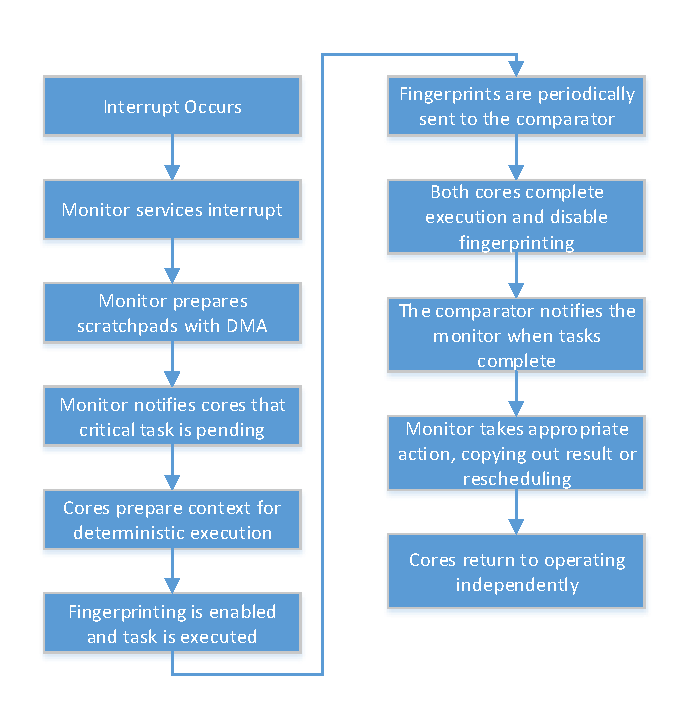
\includegraphics[scale=0.8]{Figures/control_flow}
\caption[Example of directory partitioning]{Example of directory partitioning: Task 0 reserves enough space to maintain a circular queue of size 50. Task 1 reserves a queue of size 25. And Task 2 uses the remainder of available memory.}
\label{f:control_flow}
\end{figure}


\section{Inter-core communication}

As we are dealing with a very simple real-time operating system (RTOS), it is not an easy task to implement a software only solution for message passing between cores. It is not possible to share key data structures such as event-control blocks (ECBs) between cores. An ECB is the basic data structure used by the uC/OS-II RTOS (uCOS from here on) to define mutexes, semaphores, event flags, and queues. Since the RTOS is not built to be able to share ECBs between different instances on different cores it is necessary to develop another solution. Fortunately it is fairly straightforward to create custom memory mappings with soft cores on the FPGA to provide hardware implemented message passing structures.


A 1kB region of memory is reserved for the passing of messages between cores. Furthermore, each core has a register that is addressable by the other cores that triggers an interrupt. The size of the shared memory region can be adjusted if necessary. It is also assumed that each piece of information in the shared memory at any given time is only written by one core. Access to shared memory is controlled with a hardware mutex. Listing \ref{l:mon_init} shows how the monitor core initializes certain system variables and notifies the other cores. The initialization of the plain cores is stalled until the monitor is able to set up certain global variables.

 \begin{lstlisting}[frame=single,language=C,label=l:mon_init,caption={[Monitor passes messages to other cores]The monitor core aquires a hardware mutex and uses shared memory to pass messages to the other cores}] 
 CriticalFunctionPointers* cp = (CriticalFunctionPointers*) SHARED_MEMORY_BASE;
 //Acquire the mutex
altera_avalon_mutex_lock(mutex, 1);
{
	//Set some initial start up values
	cp->critical = critical_task;
	cp->preempt = qsort_test;
	//Notify other cores that initialization is complete
	cp->init_complete = 1;
}//release the mutex
altera_avalon_mutex_unlock(mutex);
 \end{lstlisting}
Meanwhile the plain cores wait for the cp$\rightarrow$ init\_complete variable to change before proceeding with their initialization in Listing \ref{l:core_init}.

\begin{lstlisting}[frame=single,language=C,label=l:core_init,caption={[Plain core startup synchronization]Plain core waits for the initialization by the monitor to finish before updating the variables}] 
//The plain cores wait on the init_complete variable
while(cp->init_complete == 0);
altera_avalon_mutex_lock(mutex, 1);			
{
	//They load the values placed in shared memory by the monitor
	ct = cp->critical;
	pt = cp->preempt;
}
altera_avalon_mutex_unlock(mutex);		
\end{lstlisting}


In this example, the plain cores are at the beginning of their code and are using a spin lock because they all must wait until the monitor has reached a certain point in its startup before they can continue and \emph{no other work} can be done since this is the startup routine. However, \emph{all subsequent} communication between the monitor and the cores will be \emph{interrupt driven}. As previously mentioned, each core is capable of interrupting the execution of the others. Currently, communication is only one way: from the monitor to the plain cores. Listing \ref{l:mon_irq_send} shows the monitor code for causing an interrupt in the other cores and Listing \ref{l:cpu_irq} shows the response from the plain core. This method can be generalized by including a message type header at the beginning of shared memory in order to pass several different types of information. In this example it is assumed that only one type of message passes from monitor to other cores.

\begin{lstlisting}[frame=single,language=C,label=l:mon_irq_send,caption={[Monitor message passing to plain cores]The monitor core puts a message in the shared memory region and then writes to the ISR pointer variables\, triggering interrupts in the other cores.}]
int *isr_0_ptr = (int *) PROCESSOR0_0_CPU_IRQ_0_BASE;
int *isr_1_ptr = (int *) PROCESSOR1_0_CPU_IRQ_0_BASE;	
altera_avalon_mutex_lock(mutex, 1);
{
	cp->task_id0 = (5);
	cp->task_id1 = (5);
	*isr_1_ptr = 1;
	*isr_0_ptr = 1;
}
altera_avalon_mutex_unlock(mutex);
\end{lstlisting}

\begin{lstlisting}[frame=single,language=C,label=l:cpu_irq,caption={[Plain cores retrieve arguments from shared memory]The plain cores handle the interrupt and retrieve the necessary information.}]
static void handle_cpu0_interrupt(void* context) {
	unsigned short task_id;
	altera_avalon_mutex_lock(mutex, 1);
	{
		CriticalFunctionPointers* cp = 
		    (CriticalFunctionPointers*)SHARED_MEMORY_BASE;
		task_id = cp->task_id0;
		*isr_0_ptr = 0;
	}
	altera_avalon_mutex_unlock(mutex);
	if(task_id == CRITICAL_TASK_PRIORITY)
		OSSemPost(mbox);
}
\end{lstlisting}

\section{Initializing and communicating with the Comparator core}

As was already discussed in Chapter \ref{Chapter1}, the monitor core is responsible for organizing the mapping of FIDs to actual critical functions. It is not necessary for this mapping to be static and it is not possible if there are more functions than FIDs. There are two pieces of information required by the comparator in order for it to correctly interpret messages from the fingerprinting units: which core is executing a given FID, and how to partition the local memory space between tasks for the storage of fingerprints.

\subsection{The core assignment table}

The \emph{core assignment table} (CAT) is a mapping of a \emph{physical core ID} (PCID) to a \emph{virtual core ID} (VCID). The PCID is a 4 bit number that is assigned uniquely to each core and fingerprinting unit. The comparator in the current implementation is limited to the comparison of two cores and is not capable of error correction through voting. Furthermore, the FID is a 4 bit number allowing up to 16 concurrent tasks to be fingerprinted. Since each FID can only be executing on two cores at a time, a table keeps track of which two cores are executing each task. An example is shown in Table \ref{t:cat}. Here, the task with FID 0 is defined to execute on cores 0 and 1. The task with FID 1 is defined to execute on cores 1 and 3. The \emph{actual function} associated with each FID can change without changing the CAT. The equivalent code for programming the hardware is shown in Listing \ref{l:cat}.


\begin{table}
\centering
    \begin{tabular}{| l | l | l  |}
    \hline
    Task & PCID 0 & PCID 1\\ \hline
    0 & 0 & 1\\ \hline
    1 & 1 & 3\\ \hline
    2 & 2 & 0\\ \hline
    3 & 2 & 3\\ \hline
    \end{tabular}
    \caption[An example core assignment table.]{An example core assignment table. Each row is associated with a task shown in this picture for demonstration purposes; the real table only has two columns and the task is implicitly defined by the index number. }
    \label{t:cat}
\end{table}


\begin{lstlisting}[frame=single,language=C,label=l:cat,caption=The monitor programs the CAT in the comparator.]
Core_Assignment_Table ca;
//ca.table[VCID][FID] = PCID
ca.table[0][0] = 0;
ca.table[1][0] = 1;
ca.table[0][1] = 1;
ca.table[1][1] = 3;
ca.table[0][2] = 2;
ca.table[1][2] = 0;
ca.table[0][3] = 2;
ca.table[1][3] = 3;
set_core_assignment_table(&ca);
}
\end{lstlisting}

\subsection{Initializing the directory}

The next step for the monitor is to define the partitioning of the comparator's local memory space to store fingerprints. In the current implementation, the comparator has capacity to store 512 fingerprints. The 512 spaces can be divided amongst the 16 FIDs in arbitrarily sized circular queues. For instance, suppose FID 1 is associated with a function known to produce a single fingerprint. It is possible to reserve a single memory location for this task. Suppose FID 1 is known to produce over a thousand fingerprints. It may be prudent to subdivide this task into several fingerprinting intervals. However it is also possible to reserve a queue of size 50 for this task if it can be shown that the fingerprint buffer will not overflow (due to one core executing significantly faster than the other). Development of a feedback mechanism to slow down a core that is pulling too far ahead of its partner core without explicit software barriers is under way. One method of setting the directory according to this example is shown in Listing \ref{l:dir_init}. It is crucial to \emph{never} make changes to the directory structure while any tasks are being fingerprinted. For now it is the case that both virtual cores require the same directory layout, however it is still necessary to set the directory for each core individually. An example of directory partitioning is shown in Figure \ref{f:directory}

\begin{lstlisting}[frame=single,language=C,label=l:dir_init,caption=Initializing the Comparator directory.]
Directory_Init_Struct d;
//Set the directory for each virtual core
for(i = 0; i < 2; i++){
	d.core_id = i;
	//Task 0 requires a single slot
	d.key = 0;
	d.start_ptr = 0;
	d.end_ptr = 0;
	set_task_directory(&d);
	//task 1 requires several slots
	d.start_ptr = 1;
	d.end_ptr = 51;
	set_task_directory(&d);
}
\end{lstlisting}


\begin{figure}[ht]
\centering
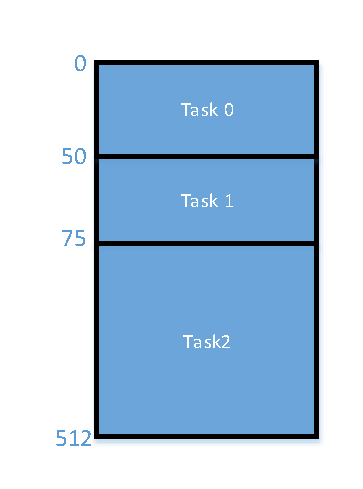
\includegraphics[scale=0.8]{Figures/directory}
\caption[Example of directory partitioning]{Example of directory partitioning: Task 0 reserves enough space to maintain a circular queue of size 50. Task 1 reserves a queue of size 25. And Task 2 uses the remainder of available memory.}
\label{f:directory}
\end{figure}

\section{Initiating a critical task with the Monitor}
Once the comparator has been properly initialized, the Monitor can begin to request the execution of critical tasks from the plain cores. Presumably the request from the monitor would itself be triggered by some interrupt. The monitor will then acquire the hardware mutex, transfer any necessary information into the scratchpads of the cores using DMA, place a pointer to the function, the FID, and any other arguments that can be user defined in shared memory, and interrupt the cores. Listing \ref{l:mon_task} shows how the monitor might initiate a critical task.
\begin{lstlisting}[frame=single,language=C,label=l:mon_task,caption={[Mointor initiates a critical task on plain cores]The monitor requests cores 0 and 1 to begin executing a function called critical\_task with FID 0.}]
altera_avalon_mutex_lock(mutex, 1);
{
	cp->function[0] = critical_task;
	cp->function[1] = critical_task;	
	cp->fid[0] = (0);
	cp->fid[1] = (0);	
	cp->blocksize[0] = 0x5ff;
	cp->blocksize[1] = 0x5ff;
	cp->args[0] = (void*)function_args;
	cp->args[1] = (void*)function_args;
	*irq_1_ptr = 1;
	*irq_0_ptr = 1;
}
altera_avalon_mutex_unlock(mutex);
\end{lstlisting}
\section{Executing a critical task with fingerprinting}
uCOS has a capacity for 256 tasks with priorities 0-255. It is not possible for two tasks to have the same priority. The simplest thing to do is to reserve tasks 0-15 for fingerprinting. Each OS task (OST) is assigned a generic wrapper that will execute an arbitrary function associated with the given FID. The identities of the function and FID are passed by the comparator as shown in Listing \ref{l:mon_task}. More flexible and powerful message passing schemes can be implemented. The method of responding to a request from the monitor is shown in listing \ref{l:cpu_response}. Some parts of the code not essential to the current discussion have been omitted.
\begin{lstlisting}[frame=single,language=C,label=l:cpu_response,caption=Plain core 0 responds to the request from the monitor.]
void (*critical_task)(void*);
int blocksize;
//Interrupt handler
static void handle_cpu0_interrupt(void* context) {
	unsigned short task_id;
	altera_avalon_mutex_lock(mutex, 1);
	{
        CriticalFunctionPointers* cp = 
            (CriticalFunctionPointers*)SHARED_MEMORY_BASE;
        //retrieve the FID of the task
		task_id = cp->fid[0];
		//retrieve the address of the function
		critical_task = cp->function[0]
		//retrieve the fingerprinting block size
		blocksize = cp->blocksize[0];
		//reset the IRQ
		*irq_0_ptr = 0;
	}
	altera_avalon_mutex_unlock(mutex);
	//Activate the appropriate OS task
	if(task_id == PRIORITY_0)
		OSSemPost(sem_0);
	else if(task_id == PRIORITY_1)
		OSSemPost(sem_1);
}

//The tlb must be used for global variable references
void init_tlb(){
	set_cputable_entry(1, GLOBAL_VARIABLE_SECTION);
	set_spmtable_entry(1, TLB_BASE);

	//Enable the translations
	set_enable(0x2);

}

//The critical task wrapper:
INT8U err;
void critical_task_wrapper(void* pdata){
	int* p = pdata;
    //The priority is assigned to the task when created by the OS
	int priority = *p;
	while(1){
		//A single task wrapper can be written for all priorities using
		//conditional waiting
		if(priority == PRIORITY_0)
			OSSemPend(sem_0, 0, &err);
		else if(priority == PRIORITY_1)
			OSSemPend(sem_1, 0, &err);
	    
	    //the critical task address is loaded onto the stack
	    void (*pt)(int) = critical_task;
		//the block size is forwarded to the fingerprint unit	    
	    fprint_set_block_size(blocksize);
	    //The TLB is initialized with the proper translation table
		init_tlb();
		//The TLB is enabled
	    enable_tlb();
		long registers[8];
		//The callee saved registers must be pushed to the stack
		// and set to 0
		context_switch(registers);
		//The global pointer is set to match the monitor core
		set_gp();
		//The critical task is executed
		critical_task(&args);
		//Restore the local global pointer register
		restore_gp();
		//Restore the callee saved registers
		context_restore(registers);
		//Turn off translation
		disable_tlb();
	}
}
\end{lstlisting}

There are several important things that happen in this code. First is the interrupt handler. This retrieves the FID and the function pointer from the shared memory region. It also retrieves the blocksize that sets the number of stores used by the fingerprint unit to calculate each fingerprint (where the size of the block affects the hamming distance and guaranteed error coverage provided by the CRC algorithm). It then signals the appropriate task wrapper based on the value of the FID. The task wrapper is the same generic wrapper for all critical tasks. Each wrapper is statically assigned a priority by the OS during startup. Each wrapper waits on its own signal. When the signal arrives from the interrupt handler, the wrapper then does several things before calling the task: it turns on the TLB, it saves and resets the context, it changes the global pointer, and then it finally calls the critical task. Recall that memory translation, GP substitution, and the setting of callee saved registers to zero prior to initiating fingerprinting are required to ensure \emph{deterministic execution}. Also note that changes are made to the initial interrupt context save routine in order to restore the GP for interrupt handlers so that these will not be broken if interrupts are not disabled during the critical task.

There is one more layer to get to the proper critical function. The issue is that fingerprinting must be enabled and disabled without storing the return address of the local wrapper function. This return address would not match on the different cores. Therefore a \emph{wrapper within the wrapper} is required. The code that enables and disables fingerprinting must be part of the shared code. Suppose that the critical task in question was an FSM control for the shift logic in a car. When the critical task is called from the wrapper in Listing \ref{l:cpu_response}, it takes the form of Listing \ref{l:critical_task}. This code, including the FSM function, are compiled for the Monitor to ensure the location of global variables are in the section of memory being translated by the TLB.

\begin{lstlisting}[frame=single,language=C,label=l:critical_task,caption=The inner layer wrapper.]
void critical_task(void* args){
	int priority = *(int *)args;
	enable_fprint_task(priority);
	    ShiftLogic_step();
	disable_fprint_task(priority);
}
\end{lstlisting}

All other activity between the fingerprinting units themselves and the comparator are invisible to the software. When the result of a comparison is ready, the Monitor is notified via interrupt. As shown in Listing \ref{l:mon_comp_int}, the Monitor uses simple functions to retrieve a status update from the Comparator. Depending on the program, further actions can be taken. It remains to be done to develop a generalized framework across the system for killing and restarting failed tasks.

\begin{lstlisting}[frame=single,language=C,label=l:mon_comp_int,caption=The monitor interrupt handler for the comparator]
static void handle_comp_interrupt(void* context) {
	int endstate[10];
	Fprint_Status status;
	fprint_status(&status);
	...
}
\end{lstlisting} 
%
\chapter{Hardware Design} % Main chapter title

\label{Chapter3} % For referencing the chapter elsewhere, use \ref{Chapter1} 

\lhead{Chapter 3. \emph{Hardware Design}} % This is for the header on each page - perhaps a shortened title

There are two hardware components required for fingerprinting: the fingerprinting unit itself and the centralized comparator. The fingerprint unit must passively monitor the data bus of a core to compute fingerprints and periodically send these fingerprints to the comparator. The comparator must pool and organize fingerprints collected from all the cores and compare them to decide if the system is operating correctly. The comparator must then notify the monitor core upon the successful completion of a task or if an error has been detected. Three interfaces must be specified: the cores to the fingerprint unit, the fingerprint unit to the comparator, and the comparator to the monitor. This section will describe these interfaces as well as cover the mechanism by which rate monotonic (RM) scheduling is supported (i.e. preemption of fingerprinted tasks) and the internal microarchitectures of the fingerprint unit and the comparator.

\section{Fingerprinting Interfaces}
\subsection{Processor/Fingerprint Unit Interface}
Table \ref{t:fprint_reg} contains the list of registers in the fingerprint unit that can be written by the processor it is attached to. Note that all address offsets are given from the perspective of the sender. The sender address offset is always shifted left by two bits compared to the offset the receiver uses. The current state register bitfield is defined in Table \ref{t:cs_bitfield}.
\begin{table}
\centering
    \begin{tabular}{| l | l | l  | p{6cm} |}
    \hline
    Register & RW & Offset & Function\\ \hline
    Current State (CS) & W & 0x0 & Used to enable and disable fingerprinting\\ \hline
    Block size (BS) & RW & 0x10 & The BS register contains the size of a fingerprinting block for the current task\\ \hline
    Pause  & R & 0x8 & The pause register is used by the interrupt trap to signal that the current task should pause its fingerprinting. The value read has no meaning.\\ \hline
    Unpause & R & 0xc & The unpause register is used by the interrupt trap to signal that the most recently paused task should resume fingerprinting. The value read has no meaning.\\ \hline
    \end{tabular}
    \caption{Fingerprint unit control registers}
    \label{t:fprint_reg}
\end{table}


\begin{table}
\centering
    \begin{tabular}{| l | l | l | p{6cm} |}
    \hline
    Name & Offset & Size(bits) & Function\\ \hline
    FID & 0x0 & 4 & The FID of the task beginning or ending fingerprinting.\\ \hline
    Enable bit & 0x4 & 1 & The enable bit signals whether fingerprinting is beginning or ending.\\ \hline
    \end{tabular}
    \caption{Current state register bitfield.}
    \label{t:cs_bitfield}
\end{table}

The functions used for this purpose are:
\begin{itemize}
\item{enable\_fprint\_task(int FID): begin fingerprinting on the given core a task with FID.} 
\item{disable\_fprint\_task(int FID): end fingerprinting on the given core a task with FID.}
\item{fprint\_set\_block\_size(int size): set the block size for the task beginning fingerprinting. Set prior to enabling fingerprinting.}
\end{itemize}

\emph{Block size:} A default value of 0xFFF is currently provided for the fingerprint unit. The block size \emph{MUST} be odd to function correctly. In anticipation of future work exploring the fingerprinting of both store and load instructions, the counter is currently set to increment by 2 since load instructions contribute half as many bits as store instructions (only the address is used). A value of 0xFFF = 4095 signifies that 2048 stores will be used to calculate a fingerprint. Each store contains 59 bits (27 address and 32 data bits). This means that each 32 bit fingerprint compresses 120832 bits of execution stream resulting in 3776x compression. A table of polynomials including block sizes over which a given hamming distance is achieved is provided in \cite{koopman200232}.
\begin{figure}
\centering
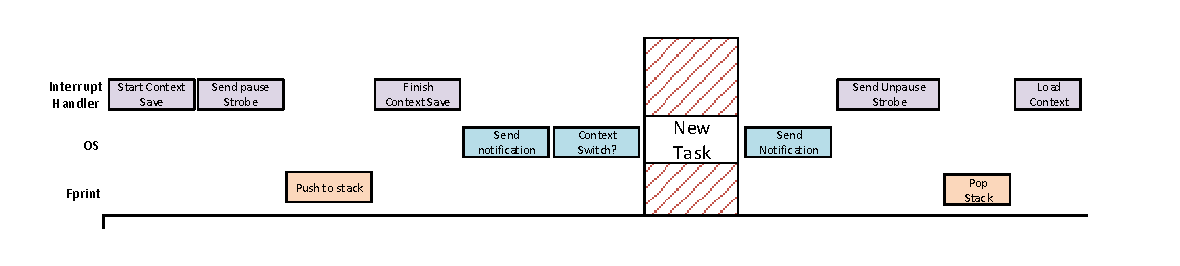
\includegraphics[scale=0.8]{Figures/interrupt}
\caption[Preemption of a fingerprinted task]{Preempting a fingerprinted task without corrupting the fingerprint. The low level assembly interrupt handler and the OS interrupt wrappers are depicted separately.}
\label{f:int}
\end{figure}
\emph{Pausing: } 	At times it may be necessary for one critical task to preempt another. 
	In the context of fingerprinting, this presents additional challenges:
		the fingerprinting of the preempted task must not be disrupted, but the fingerprinting logic must be available for the new task.
	Figure \ref{f:int} shows the procedure.
	First, the interrupt vector responsible for context saving located in the BSP is modified to send a strobe to the fingerprint unit notifying it that it should stop fingerprinting.



	The problem arises that there is no way for communication between software and hardware to occur without the software corrupting its own context (it must load the address of the hardware into a register). 
	We propose a convention whereby the fingerprinting hardware is able to roll back its calculations by one iteration, thus allowing a single store instruction to be executed without corrupting the fingerprint. 
	When an interrupt occurs, the initial context saving assembly routine is modified to store exactly one register onto the stack, and then this register is used to load the address of the fingerprint unit pause strobe (Listing \ref{l:int_trap_st}). 
	
		\begin{lstlisting}[frame=single,language=C,label=l:int_trap_st,caption=The updated trap at the start of an interrupt.]
stw   ra,  0(sp)
movhi ra,  \%hi(0x8100000)
ori   ra,  ra, 8
ldw   ra,    0(ra)
stw   r1,   8(sp)
stw   r2,  12(sp)
...
\end{lstlisting}

	The fingerprint unit rolls back its calculation by one iteration when it receives the pause strobe. 
	Following this, the RTOS has its own interrupt wrapper functions. The OS notifies the fingerprint unit that it is about to call the context switch routine.
	If a higher priority task is ready, then it will execute in its entirety.
	When the context switch function finally returns, the OS again sends another notification to the fingerprint unit. 
	Finally an unpause strobe is included in the context restore vector in the BSP (Listing \ref{l:int_trap_ld}).
	\begin{lstlisting}[frame=single,language=C,label=l:int_trap_ld,caption=The updated trap at the end of an interrupt.]
movhi ra,  %hi(0x8100000)
ori   ra,  ra, 12
ldw   ra,    0(ra)
ldw   r5,  68(sp)
ldw   ea,  72(sp)  
ldw   ra,   0(sp)
...
\end{lstlisting} 
	The main purpose of the OS notification is to guard against unwanted behaviours that may arise due to nested interrupts. It is possible to imagine other types of communication passing between the OS and the fingerprinting unit once fingerprinting has been successfully paused. 
	For instance, the fingerprinting unit currently only supports rate monotonic scheduling and stores paused task context on a stack. 
	It is reasonable for the OS to pass messages to the fingerprinting to notify it which task is being resumed and for the hardware stack to be replaced by a more flexible data structure. 
	There are potential issues here in that the unreliable core is now passing information to the FP unit that may affect the fingerprinting of several tasks if it is not done properly. 
	We do not explore this issue in any greater detail but note that this behaviour is easily supported by the hardware should it be desired.
%
%
%
%Corrupting the context is not an issue at the end of the interrupt. The unpause strobe can simply be activated before loading back the original context. It must be the case that no interrupt related stores occur after the unpause strobe. If stack exceptions are enabled, for instance, the location of the pause strobe would have to be slightly altered. Listing \ref{l:int_trap_ld} shows the unpause strobe in the trap.
%
%
%The last thing that should be mentioned with respect to pausing is that there is also a uCOS wrapper that is executed prior to the user defined interrupt handler. This can be modified in future versions to send more information from the OS to the fingerprinting unit about the task to be resumed. Figure \ref{f:exception_flow} shows the software flow of exception handling in the Nios system. Once fingerprinting is paused, the OS Interrupt Exit function can be modified to send more details to the fingerprinting unit using as of yet unspecified control registers.

%\begin{figure}[h]
%\centering
%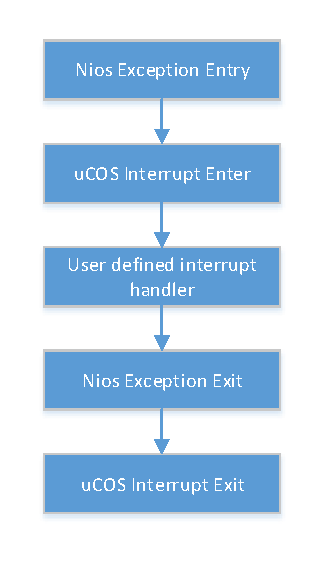
\includegraphics[scale=0.8]{Figures/exception_flow}
%\caption{Exception software flow in Nios II system.}
%\label{f:exception_flow}
%\end{figure}

\subsection{Fingerprint unit/Comparator Interface}
Messages are passed from the fingerprinting unit to the comparator when a task begins, when a fingerprint is complete, and when a task ends. The pausing of tasks is invisible to the comparator. Task begin/end messages can be sent in a single packet. Fingerprints require two packets to be sent to the comparator. The type of message being sent and the identity of the sender are encoded in the lower bits of the address. Table \ref{t:msg_format} shows the format for these messages. The size of each field could potentially be changed to satisfy different platform criteria. The messages could also be divided into two packets if the size of the offset becomes unreasonably large.
\begin{table}[h]
\centering
    \begin{tabular}{| l | l | l | l | l | }
    \hline
     & Base Address & Core ID & Message Type & Pad\\ \hline
    Message & 17 bits & 4 bits & 4 bits & 2 bits (0)\\ \hline
    \end{tabular}
    \caption{Message type format for sending messages from the fingerprint unit to the comparator.}
    \label{t:msg_format}
\end{table}
\begin{table}[ht]
\centering
    \begin{tabular}{| l | l |}
    \hline
    Message Type & Value\\ \hline
    Status update & 0\\ \hline
    Fingerprint & 4\\ \hline
    \end{tabular}
    \caption{Message type values for sending messages from the fingerprint unit to the comparator.}
    \label{t:msg_types}
\end{table}

The possible values for the current message types are shown in Table \ref{t:msg_types}. In the case of sending a fingerprint, it is necessary to break the 32 bit CRC up into two messages in order to be able to send the FID of the task that generated the fingerprint as well.  The format for sending fingerprints over two packets is shown in Table \ref{t:fprint_format}.

\begin{table}[h]
\centering
   \begin{tabular}{| l | l | l | l | }
    \hline
     & Partial Fingerprint & Packet & FID\\ \hline
    Lower half & 16 bits & 12b'0 & 4 bits\\ \hline
    Upper half & 16 bits & 12b'10 & 4 bits\\ \hline
    \end{tabular}
    \caption{Format for sending 32 bitfingerprints in 2 packets.}
    \label{t:fprint_format}
\end{table}


\subsection{Comparator/Monitor Interface}

Table \ref{t:comp_reg} contains the list of registers in the Comparator unit that can be accessed by the monitor core. The directory stores the offsets for start and end pointers of a circular queue and the addressing convention is given in Table \ref{t:dir_format}. The format for setting the core assignment table is shown in Table \ref{t:cat_format}. Each entry in the table is given by a unique address and addressing assumes that the size of the individual entry is 4 bytes even if the physical size of the memory is different (i.e. line 0 is at 0x0 and line 1 is at 0x4 regardless of the size of a line). Note that all address offsets are given from the perspective of the sender. The sender address offset is always shifted left by two bits compared to the offset the receiver uses.

The functions available to the monitor are:
\begin{itemize}
\item{fprint\_reset\_irq(void): Resets the status, fail and success register.} 
\item{set\_task\_directory(Directory\_Init\_Struct*): Set an entry of the directory.}
\item{fprint\_status(Fprint\_Status* fps): Retrieve the value of the three control registers.}
\item{set\_core\_assignment\_table(Core\_Assignment\_Table* ca): Sets the entire core assignment table.} 
\end{itemize}

\begin{table}
\centering
    \begin{tabular}{| l | l | l | p{8cm} |}
    \hline
    Register & RW & Offset & Function\\ \hline
    Status & RW & 0xC0 & Bit 6 is IRQ bit. Other bits reserved for future use.\\ \hline
    Success  & R & 0xC4 & Each bit of the success register is set to 1 when the corresponding task completes successfully. The register is automatically cleared when the status register is written to.\\ \hline
    Fail & R & 0xC8 & Each bit of the fail register is set to 1 when an error is detected in the corresponding task. The register is automatically cleared when the status register is written to.\\ \hline
    \end{tabular}
    \caption{Comparator control registers}
    \label{t:comp_reg}
\end{table}
\begin{table}
\centering
    \begin{tabular}{| l | l | l | l | p{6cm} |}
    \hline
    Name & RW & Offset & size & Function\\ \hline
    Start Pointer & W & 0x40 & 0x20 & Store the start pointers for each task: task 0 at offset x040, task 1 at offset 0x44, etc.\\ \hline
    End Pointer & W & 0x80 & 0x20 & Store the end pointers for each task: task 0 at offset x080, task 1 at offset 0x84, etc.\\ \hline
    \end{tabular}
    \caption{Comparator directory addressing format}
    \label{t:dir_format}
\end{table}

\begin{table}
\centering
    \begin{tabular}{| l | l | l | l |}
    \hline
    Address & VCID (1 bit) & Base Offset (6 bits) & Pad (2bits)\\ \hline
    Data & FID (4 bits) & PCID (4 bits) & Pad (2 bits)\\ \hline
    \end{tabular}
    \caption{Comparator Core Assignment table addressing and data format}
    \label{t:cat_format}
\end{table}

\section{Custom IP Microarchitectures}
This paper has taken a top-down approach in specifying the fingerprinting capable platform. First came a general overview of some important trends in dependable system design including two important examples: a reliable MPSoC and a hypervisor for partitioning of mixed critical systems. Following this, the software control flow was explored in greater detail in order to understand how fingerprinting services could be integrated into application or hypervisor code. This Chapter has so far covered the interfaces between each pair of agents in the system that are able to communicate with each other. A fairly complete \emph{black-box} description of the fingerprinting and comparator units has been established. It is now possible to examine the design of these peripherals at the register-transfer level.

\subsection{Fingerprint Unit}
There are three ports to the fingerprinting unit, as shown in Figure \ref{f:fprint_icon}. There is an addressable slave port for accessing the control registers, a port connected to the data bus directly (bypassing any bus translation and routing logic) used to calculate fingerprints, and a master port for sending information to the comparator.

Figure \ref{f:fprint_sch} shows the schematic for the fingerprint unit. The behaviour of the fingerprint unit is broken down into three independent FSMs. This will make future modifications to the pause or message passing protocols easier as they are independent of each other. Also, notice that the three variables stored in the fingerprinting unit, the FID, the counter value, and the fingerprint itself all have stacks associated with them. When a task is paused, the state of these three registers are pushed onto their respective tasks. Before the unpause strobe occurs, a new task can begin fingerprinting without corrupting the state of the previous task. The stack currently has a depth of eight. The LIFO structure is valid since we are only considering support for schedules with RM scheduling.


\begin{figure}[h]
\centering
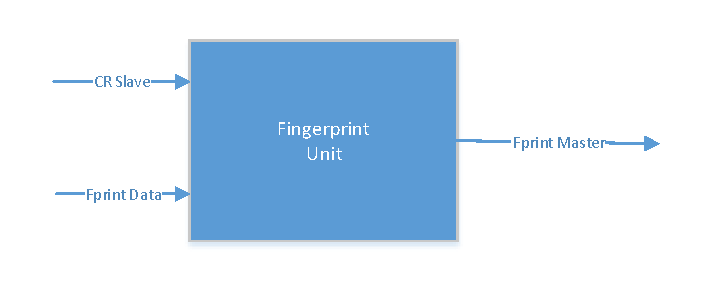
\includegraphics[scale=0.8]{Figures/fprint_icon}
\caption{Fingerprint unit ports.}
\label{f:fprint_icon}
\end{figure}

\begin{figure}[ht]
\centering
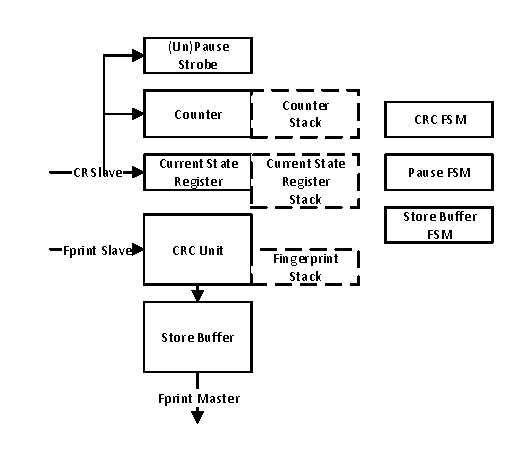
\includegraphics[width=10cm]{Figures/fprint_sch}
\caption{Schematic of the fingerprint unit components.}
\label{f:fprint_sch}
\end{figure}


\subsubsection{CRC Implementation}
The CRC implementation is shown in Figure \ref{f:crc}. A detailed explanation of how the CRC circuit is derived can be found in \cite{Hamed:12}. The circuit has been further modified to allow a \emph{variable} input data width. The implementation hinges on the RTLA multiplexers. For a $W$ bit circuit there will be $RTLA_i$ multiplexers indexed $1 < i < W$.
For an $M$ bit fingerprint, it is possible to shift the values in the RTLA to the right such that only the upper part of the circuit is used. This is useful for future implementations when load and store instructions will be used. For load instructions, only the address will be fingerprinted. By ensuring that the upper bits of the input $A_i$ are the address bits from the bus, it is possible to keep the block from being overly padded with zeros. In Figure \ref{f:rtla}, (a) shows the original RTLA while (b) and (c) show the updated RTLA capable of updating the fingerprint of either the address or the address and data inputs depending on whether or not the instruction is a store or a load. 

\begin{figure}[ht]
\centering
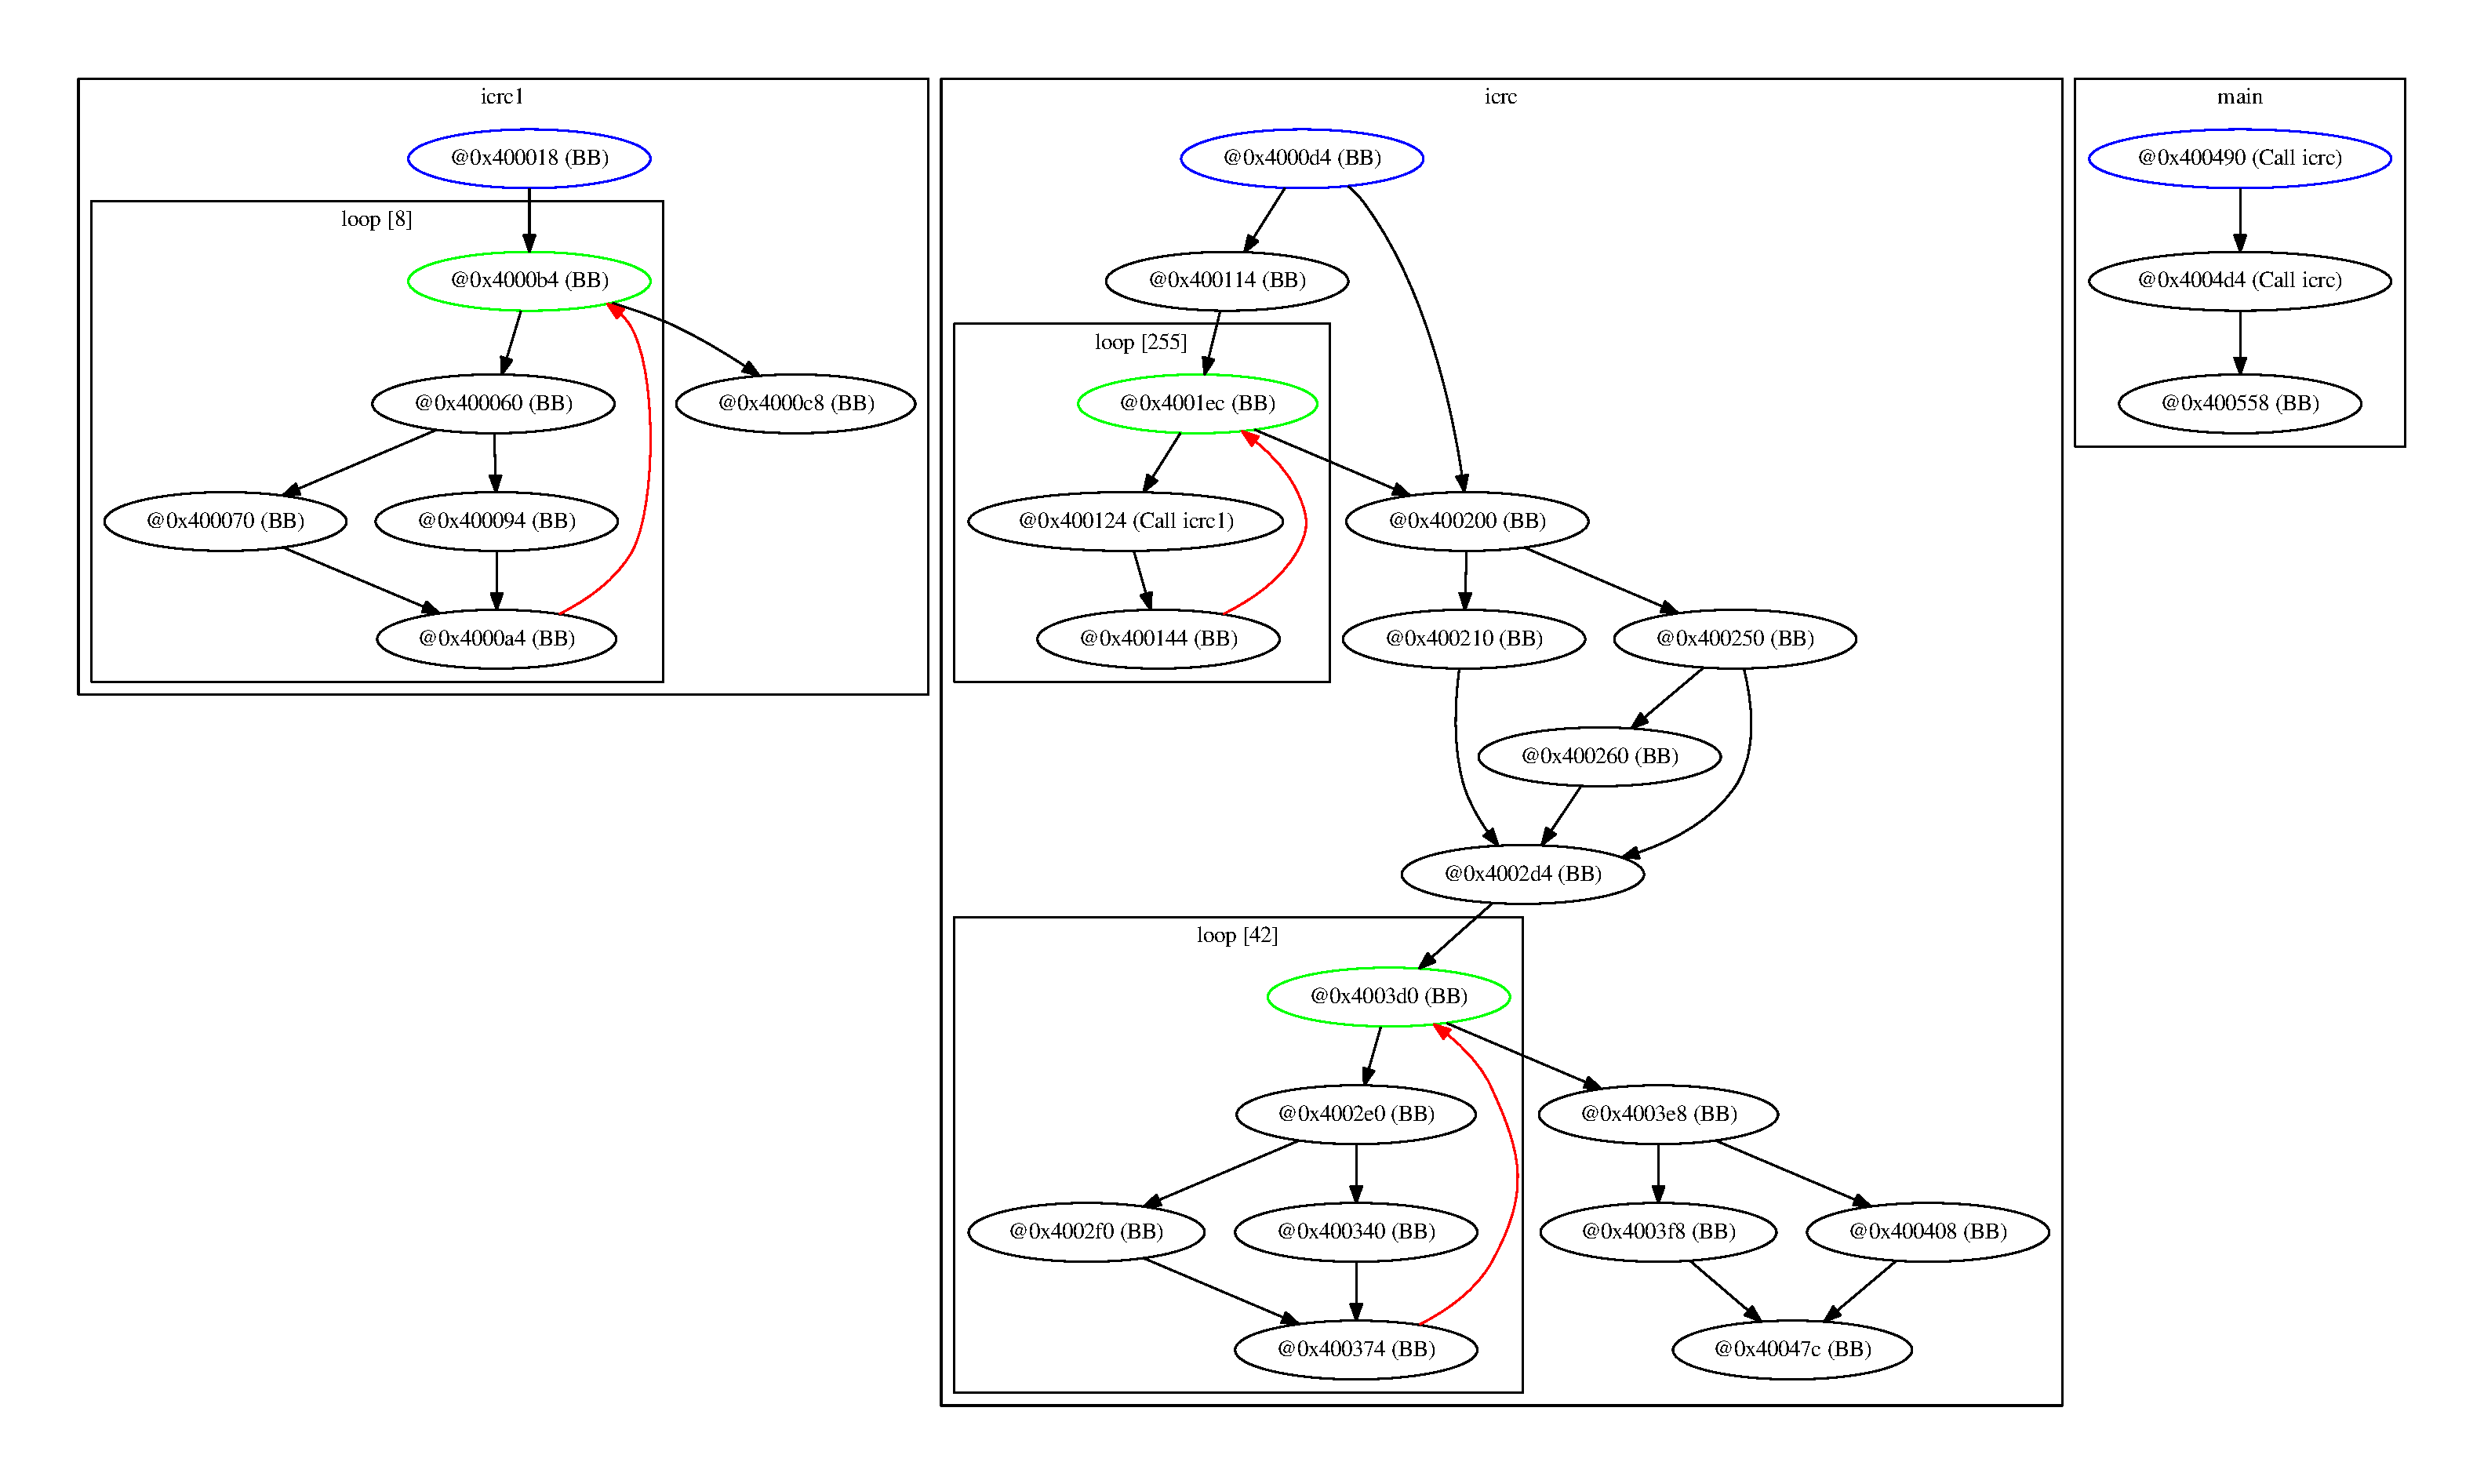
\includegraphics[width=10cm]{Figures/crc}
\caption{Implementation of CRC algorithm.}
\label{f:crc}
\end{figure}

\begin{figure}[ht]
\centering
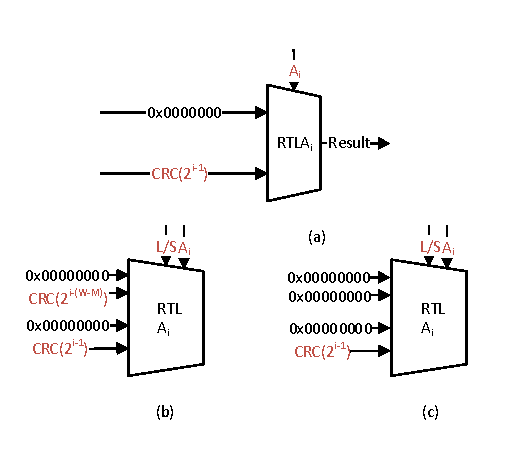
\includegraphics[scale=1]{Figures/rtla}
\caption[RTLA modification]{\emph{RTLA modification:} (a) original RTLA. (b) The RTLA for the upper portion of the input. When a load instruction is being fingerprinted the lower RTLA values are shifted right. (c) The lower portion of the input is completely deactivated during load instructions.}
\label{f:rtla}
\end{figure}

\subsubsection{Preventing state corruption during pause}
As was already discussed in Chapter \ref{Chapter2}, it is not possible to pause fingerprinting without causing at least one erroneous store instruction. Therefore each state register is doubled in order to store the \emph{previous} value to the latest calculation. It is the previous value that is pushed onto the stack to be restored when a task is unpaused. Furthermore, it is important to ensure that there are mechanisms to catch whether the erroneous store \emph{completes} a fingerprinting block. In the current implementation, the store buffer holds onto fingerprints until either a pause strobe or any other event occurs that changes state. The fingerprint is discarded if a pause strobe is the next event. Otherwise it is sent to the comparator. 

\subsection{Comparator}
The comparator collects fingerprints from all the cores in a system and compares them. The current implementation of the comparator is limited to 16 cores and two-way comparison. Ideas previously discussed in the interface sections as well as Chapter \ref{Chapter2} will receive less thorough treatment. Figure \ref{f:comp_sch} shows the comparator schematic with all the main components. Figure \ref{f:comp_fsm} shows the comparator FSM. The implementation of the comparator is quite involved and somewhat counter-intuitive and the best way to understand how it behaves as a whole is to directly examine the Verilog code. A summary of each state will be given. Three new data structures must first be introduced: the \emph{Fprint Trigger} register and the \emph{Checkin and Checkout} registers, and the \emph{Head and Tail Pointers}.

\begin{figure}[ht]
\centering
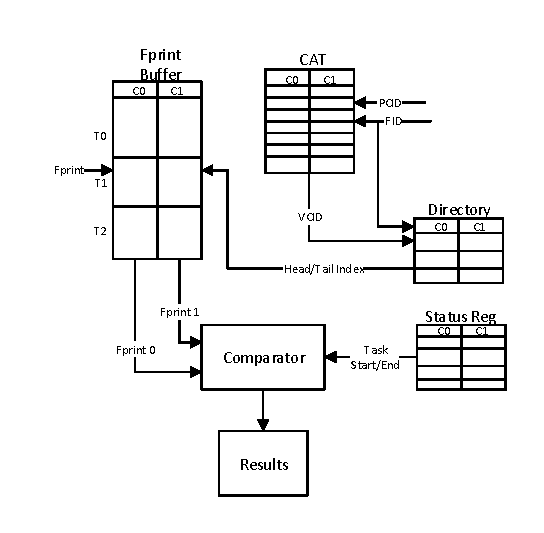
\includegraphics[scale=1.5]{Figures/compsch}
\caption[Comparator schematic]{\emph{Comparator schematic:} The FID, PCID and fingerprint arrive from the fingerprint unit. The FID and PCID are embedded in the address offset. The CAT is used to determine the VCID. The directory uses the VCID to locate the head pointer for the given FID. The comparator communicates with all the data structures but these signals have been omitted for clarity.}
\label{f:comp_sch}
\end{figure}
The \emph{Fprint Trigger} register keeps track of when the first new fingerprint arrives for a task since the last fingerprint was compared. This register is necessary because the arrival of a fingerprint is not in itself an event that should trigger comparison. Only once new fingerprints are available from both cores should a comparison be done. Also, in the case where a comparison cannot immediately be serviced, for instance if fingerprints arrive from several different tasks at once, the comparator can easily keep track of what is left to be done. The \emph{Checkin and Checkout} registers are simply registers that maintain a record of whether a task has started or ended on either of the virtual cores. The \emph{head and tail} registers keep track of the position of each task within the fingerprint queue. Remember that each task has its own start and end pointers that define a subset of the total fingerprint memory for a circular queue.

\begin{enumerate}
\item{\emph{Init:} The comparator is in an initial wait stage until an event occurs. Either a task has completed or a fingerprint has arrived.}
\item{\emph{Set Task:} The FID that caused the event is retrieved.}
\item{\emph{Load Pointer:} The tail pointer of the associated FID is loaded}
\item{\emph{Load Fprint:} The fingerprints are retrieved from the fingerprint buffer using the tail pointer.}
\item{\emph{Check Task Status:} If the checkin is activated for the given FID, then the task has completed(State 6). Otherwise proceed to State 7 to compare fingerprints.}
\item{\emph{Task Complete:} If the two head pointers match, then the same number of fingerprints arrived for both cores and the task was successful. Otherwise there was a problem (but no comparison took place because the comparator waits for new fingerprints from \emph{both} cores.}
\item{\emph{Compare Fprints:} If the fingerprints match then the tail pointer should be incremented (State  10). Otherwise a mismatch is detected.}
\item{\emph{Mismatch Detected:} An error has occurred.}
\item{\emph{Task Verified:} The task has been verified.}
\item{\emph{Increment Tail Pointer:} After a fingerprint comparison occurs, it is necessary to increment the tail pointer to proceed to the next comparison.}
\item{\emph{Check if Done:} This state checks whether for some reason several fingerprints were waiting to be compared, in which case the next comparison occurs. Otherwise the Fprint Trigger bit for the current FID is reset.}
\item{\emph{Reset Fprint Trigger:} Reset the Fprint Trigger bit for the current FID.}
\item{\emph{Reset Head and Tail:} The head and tail pointers for the given task should be reset when an error occurs.}
\item{\emph{Write Status Reg:} The status register should be updated and an interrupt will be sent to the Monitor. Further updates to status register can be made up until the monitor responds to the interrupt.}
\end{enumerate}




\begin{figure}[ht]
%\centering
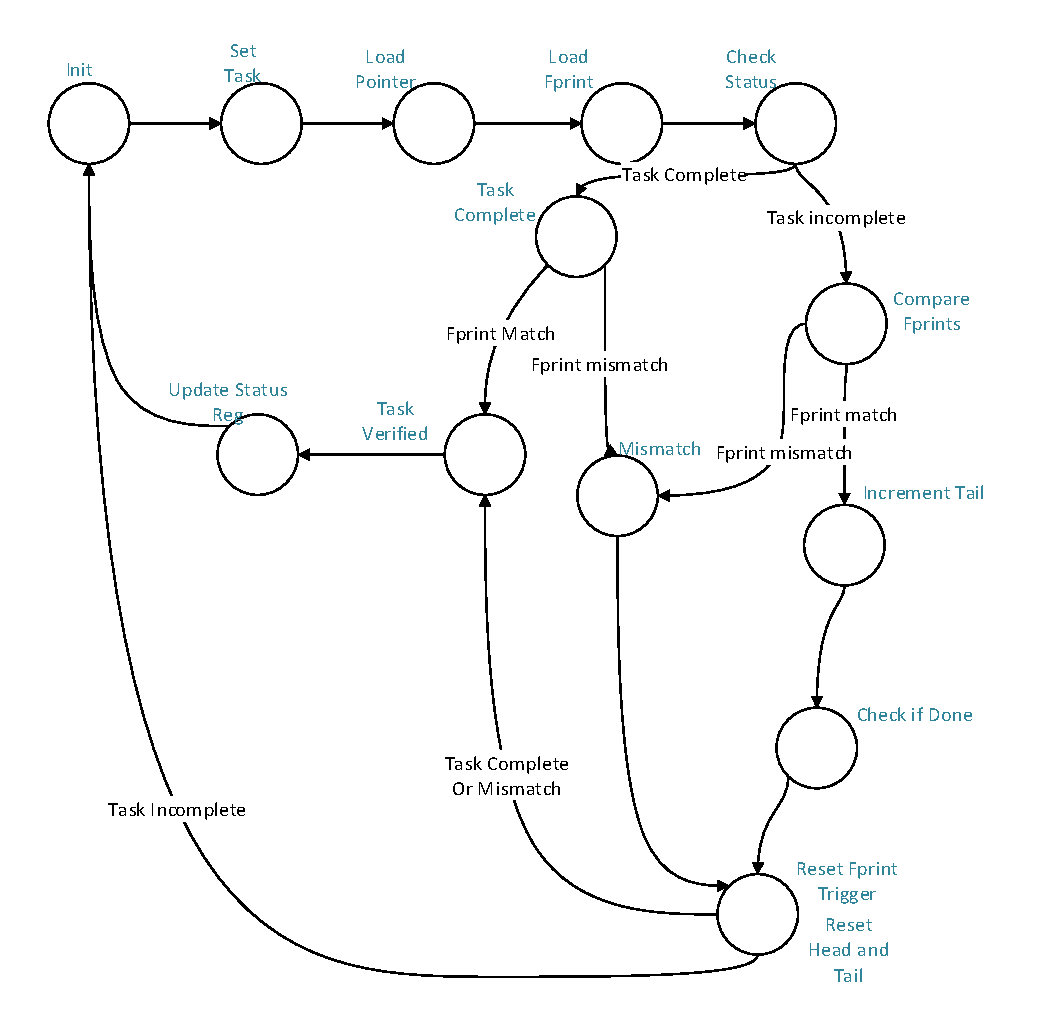
\includegraphics{Figures/comp_fsm}
\caption{Comparator FSM}
\label{f:comp_fsm}
\end{figure}



%
\chapter{Open Virtual Platform Model and Multicore Debugging} % Main chapter title

\label{Chapter4} % For referencing the chapter elsewhere, use \ref{Chapter1} 

\lhead{Chapter 4. \emph{Virtual Platform Model and Multicore Debugging}} % This is for the header on each page - perhaps a shortened title

\section{Virtual Platform Overview}
Several important and interrelated trends in embedded systems that are forcing designers to reconsider basic issues of design and verification methodologies. Firstly, there is the emergence of distributed real-time applications running on integrated multicore platforms. Secondly, there is the necessity of hardware software co-design: the platform and application development must often take place in parallel. Thirdly, heterogeneous MPSoCs, systemswith different types of cores and hardware accelerators, provide a wide range of power and efficiency tradeoffs where the optimal mapping of application to resources must be aware of the platform resources. There is also the emerging area of reconfigurable computing where the hardware and software can adapt and reconfigure based on changing system state, thus adding an extra layer of flexibility and complexity to the picture of the heterogeneous platform.

The emergence of increasingly complex architectures makes testing and verification significantly more difficult. This is compounded by the need to be able to begin software verification prior to platform availability. Furthermore, the iterative design process can be more tightly executed when these stages are done in parallel. Often, many types of problems can be anticipated in early stages of design. It is easy to iamgine a situation where hardware is designed in isolation prior to software and problems are discovered during the early stages of software development that could easily be fixed by adjusting the hardware requirements. This cannot be done if they are developed in series since by that point the development of the hardware will be too far along to allow large structural changes. If they are designed in parallel, then optimal solutions that take into account both hardware and software adjustments can be considered and large trade-off decisions can be made with a fuller picture of the system in mind.

This has led to the development of increasing sophisticated and powerful platform simulation environments. Commercial products such as Imperas Multicore Development kit based off the Open Virtual Platform (OVP) standard as well as Mentor's Questa Multicore Simulator suggest that the debugging of distributed embedded software on virtual platforms is growing in popularity. 

With all that said, this project is much more modest in scope and may not have required platform virtualization if a team with more experience had tackled the software and hardware design in isolation. Being an inexperienced designer and having no background in formal testing or verification, it was very difficult to develop a comprehensive testing strategy for the hardware. This was very much an iterative learning process. The size of the project came to encompass both hardware and software. The possibility arose for bugs in the software or hardware in isolation, or due to a lack of understanding or foresight as to how the interface between hardware and software might behave. But there was no easy way to test the two halves of the problem in isolation, stimulating them with test vectors that approximated the other half. Quite a bit of progress was made over the first year, but quite a bit of time was also wasted. Confidence disappears and paranoia sets in when you are unsure if the current solution to the problem will work, even if executed perfectly. This lack of confidence can be a tremendous burden when strange behaviours are noticed in the system that can simultaneously arise from several bugs in the software and hardware as well as miscalculations in the initial conception. This is exacerbated by a lack of visibility into the system and no ability to isolate components and recreate system wide states. There's just a single ugly knot that needs untying and no obvious place to start loosening it.

\section{OVP Overview}

Platform virtualization with OVP provides several capabilities that have dramatically increased productivity when debugging new features since its development. The basic OVP workflow is shown in Figure \ref{f:ovp} Firstly, there is full system visibility. Breakpoints can be placed at any point in the code of any processor. Secondly, peripherals are treated as processor models. They are independent code threads activated by the simulator, meaning that they can also be debugged and breakpoints inserted in their functional model. Complex chains of events can be monitored automatically using scripts and full system visibility that are not possible when running on an FPGA. Full traces of all processors can be captured. Peripherals can be distilled to their most basic functional description while also presenting to the processors exact and identical control register interfaces. Code compiled using the Nios IDE given a QSYS generated platform specification runs with no modifications on the OVP platform derived from the same specifications. Functional verification of the hardware software interface can take place with much greater ease. Especially in the case where a bug arises out of an interaction between some software and hardware element, since in the virtual platform hardware is translated into software, it is much more easy to visualize, isolate, and remedy the problem.

\begin{figure}[h]
\centering
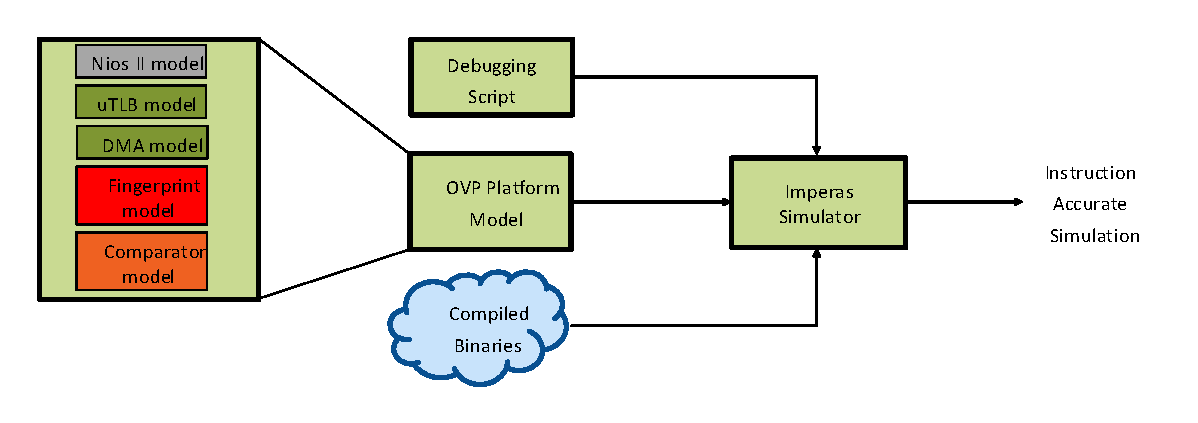
\includegraphics[scale=0.8]{Figures/ovp}
\caption{Platform virtualization workflow}
\label{f:ovp}
\end{figure}

\section{Processor Model}

The OVP processor model for the Nios II processor was co-developed with Altera and is fairly complete. Since the simulator is instruction accurate and does not take into account timing issues, the cache is omitted. Memory protection and memory management are available. One crucial aspect of the OVP system is that it is fully open source, allowing for modifications to the processor model to be made with relative ease. 

Fingerprinting involves a very strange type of peripheral that is concerned with all bus activity regardless of whether or not it is being addressed. Neither Quartus or OVP includes a built in mechanism for specifying a peripheral with this property. Therefore, it was note a trivial task to prepare the initial platform model that included a fingerprinting peripheral. 

The solution to the problem is ugly and is probably inefficient from a simulation speed perspective but it works and the technical details will now be discussed.

\subsection{Imperas Binary Intercept Technology}

In the OVP model, there are two types of behavioural descriptions: morph-time and run-time. The morph-time  API is used when creating a model description for the simulator to load the model. The run-time API is used to initiate behaviours while the simulator is running. Furthermore, there is a separate peripheral simulation engine (PSE). As it turns out, the processor simulation environment does not provide an easy way to do a seemingly simple thing. It is possible to add outgoing nets from a processor (although this is generally not done because the only outgoing signals from a processor should be the bus and buses have their own distinct model and port type). It is not possible to add to an instruction a command that stimulates one of these nets. 

Here is a more concrete example. The bus object in simulation is quite an abstraction and there is no way for a peripheral to see what is happening unless it is directly addressed. Therefore one solution is to add outgoing nets to the processor, and to modify the store instruction to stimulate those nets with information about the bus. The problem is that the code which defines the store instruction behaviour is considered morph-time by the simulator. Even if run-time APIs are included they will not be run after the simulation initializes. While it is possible to add nets to a processor, it is not possible for the processor to write values to those nets when executing store instructions. 

The Imperas Binary Intercept Technology (BIT) is a tool that allows additional run-time specifications to be added to a model as a separate shared library when the model is being loaded by the simulator. It is possible to use this tool to intercept and alter instructions as well as to monitor the system with complex chains of assertions. This is the API from which Imperas has developed their own prepackaged set of verification libraries (VAPs) and is therefore very powerful and able to reach deeply into the simulation environment.

The BIT provides two behaviours that allow the custom nets to convey information about writes. Firstly, it is possible to create a watchpoint over the entirety of memory for each core in the system. Whenever a write instruction is executed, this watchpoint is triggered. The callback of this watchpoint can then identify the processor that issues the instruction, as well as the address and data. It can then stimulate the nets associated with that processor such that they provide the information that a store has occurred as well as the address and data. These nets can then be directly connected to a fingerprinting peripheral. The BIT constructor and callback are shown in Listing \ref{l:vmi_callback}. Notice that the nets can carry 32 bit numbers, therefore three nets can carry all the information about a store instruction and that the run-time API (vmirt...) functions correctly.

\begin{lstlisting}[frame=single,language=C,label=l:vmi_callback,caption=VMI Memory watchpoint constructor and callback.]
//
// Constructor - install read and write callbacks on processor data domain
//
static VMIOS_CONSTRUCTOR_FN(constructor) {
    memDomainP domain   = vmirtGetProcessorPhysicalDataDomain(processor);
    Uns8       bits     = vmirtGetDomainAddressBits(domain);
    Addr       highAddr = (1ULL<<bits)) - 1;
    vmirtAddWriteCallback(domain, 0, 0, highAddr, writeCB, object);
}
static VMI_MEM_WATCH_FN(writeCB) {
    // we are interested only in writes made by processors (not artifacts of
    // simulation or memory accesses by other plugins, for example) so take
    // action only if processor is non null
    if(processor) {
        vmirtWriteNetPort(processor, vmirtGetNetPortHandle(processor, 
                "fprint_write_out_address"), address);
        vmirtWriteNetPort(processor, vmirtGetNetPortHandle(processor, 
                "fprint_write_out_data"), *((unsigned *)value));
        vmirtWriteNetPort(processor, vmirtGetNetPortHandle(processor, 
                "fprint_write_out"), 1);
    }
}
\end{lstlisting}

\section{Peripheral Models}
It was necessary to model the Altera provided DMA, mutex, as well as modify a prepackaged model of the Altera system timer. It was further necessary to model the comparator, the fingerprinting unit, the custom TLB, and the intercore IRQ bridge. The comparator and fingerprinting unit, including register sets, have been discussed already in some detail. This section will will give an overview of the DMA core and the TLB. The IRQ bridge is simply a bunch of register connected to the IRQ inputs of each core. Similarly the mutex is just a single register. All other functionality related to mutex behaviour is implemented in the sofware driver. Some simulation specific modifications will also be discussed.

\subsection{DMA}
A functional model of the DMA core was derived from the specification given in \cite{altera_ip_ug}. The timing characteristics of the DMA and any features related to packet size were omitted. The DMA peripheral therefore consists of one thread and one callback function that is triggered when the control register is written to by a processor. In line 4 of Listing \ref{l:dma}, the control register callback checks if the "GO" bit in the control register is written and if the length register has a non zero value (these functions should be self explanatory). If so, an event is triggered, causing the main DMA thread (line 21) to proceed past its wait condition. It should be fairly clear without any specific knowledge of the API that the main thread then updates its BUSY bit, performs the entire memory transaction in a single burst. Finally it updates all of its status bits. and notifies the processor with an interrupt if interrupts are enabled.

\begin{lstlisting}[frame=single,language=C,label=l:dma,caption=DMA model.]

PPM_REG_WRITE_CB(regWr) {
    *(Uns32*)user = data;
    if(DMACSP_ab8_data.control.bits.GO == 1 && DMACSP_ab8_data.length.value > 0){
        bhmTriggerEvent(start);
    }
}

static void dmaBurst(void) {   
    Uns32 len = DMACSP_ab8_data.length.value;
    char* buff = malloc(len);
    ppmReadAddressSpace (handles.MREAD,  DMACSP_ab8_data.readaddress.value, 
        len, buff);
    ppmWriteAddressSpace(handles.MWRITE, DMACSP_ab8_data.writeaddress.value, 
        len, buff);
    free(buff);
    DMACSP_ab8_data.length.value = 0;
    DMACSP_ab8_data.status.bits.LEN = 1;
}

static void channelThread(void *user)
{
    while(1) {
         bhmWaitEvent(start);
        
        //Start transaction
        DMACSP_ab8_data.status.bits.BUSY = 1;
         dmaBurst();
        DMACSP_ab8_data.status.bits.BUSY = 0;
        DMACSP_ab8_data.status.bits.DONE = 1;
        DMACSP_ab8_data.status.bits.REOP = 1;
        DMACSP_ab8_data.status.bits.WEOP = 1;
        if(DMACSP_ab8_data.control.bits.I_EN == 1){
            ppmWriteNet(handles.DMA_IRQ, 1);   
        }
    }
}
\end{lstlisting}

\subsection{TLB}
While the processor model comes equipped with an MMU, the translation process is completely transparent from the point of view of the intercept library and therefore there would be no easy way to integrate the TLB for fingerprinting purposes directly into the model. The same problem occurs with the actual HDL because the Nios core is encrypted. Keep in mind that for fingerprints to match, when main memory is used to store redundant state rather than dedicated scratchpads, the virtual address is required for fingerprint calculation.

The code for the TLB is a bit more cumbersome. It depends on a simulation object called a dynamic bridge that creates mappings from one address to another when a peripheral has both a master and slave port. An incoming address on the slave will continue on to the new translated address defined by the bridge. There is no thread or activity as with the DMA. There is no callback associated with the virtual address. There is no local memory object in the TLB associated with that address. The processor's fingerprinting nets are still activated by the intercept library. The TLB functions as follows:
\begin{itemize}
\item Wait until the TLB is enabled
\item Create a dynamic bridge for each translation entry in its table
\item Sort the table
\item Fill in the remainder of the address space with dynamic bridges that do not translate.
\end{itemize}

\section{Compensating for Simulation Artifacts}

The series of dynamic bridges breaks the intercept library to some extent. Simulation artifacts arise that cause fingerprints to stop matching. Both the physical and virtual address arrive at the fingerprinting unit, and sometimes several copies of them can arrive. Therefore, an interface between the TLB and fingerprinting unit must be added in order to allow the fingerprinting unit to know when translation is on and which addresses are being translated so that it ignores the physical addresses. Also, if the same data and address arrive twice in a row, it is assumed to be an artifact and is ignored. In the rare event where a program writes the same data to the same address on consecutive stores, the model simply falls a bit short in terms of its faithfulness to the physical platform. The model is very slow and running simulations in this fashion are not ideal for doing actual fault injection simulations. As a result, there is not much concern at the moment if an injected fault, once we begin developing OS services to replicate and restart threads, is masked on extremely rare events by this defective behaviour. 


\section{Case Study: Generated Code}
\label{s:matlabstudy}

\subsection{Fingerprinting a Simulink generated control loop}
Model based design is fundamental to automotive software engineering. An increasing proportion of the millions of lines of code that are currently used to run modern cars are computer generated \cite{mossinger2010software}. Furthermore, whether soft core or hard core, ISAs are established and compiler tool chains are mature and stable. One advantage of this architecture over single core hardening techniques is that no access or changes to existing core designs are required at the microarchitectural level. It is similarly advantageous to be able to leverage existing compiler and model-based code generation tools without requiring modifications. This second example demonstrates how fingerprinting can be used to monitor redundant executions of Simulink generated control code integrated into a simple RTOS template and compiled with \emph{gcc}.

Simulink Coder was used to extract transmission control logic from an example of an automotive drive train model \cite{sim_trans}. It would defeat the purpose and convenience of Coder to be forced to comb through and restructure the code to obey some style that is not natively supported. There are two things to note about the style of code: one that supports ease of fingerprinting and one that requires more attention. Firstly, the algorithm is a discrete FSM that will deterministically produce the same outputs given identical inputs. The tasks will match at the instruction level. The areas requiring more attention is the handling of global variables. Since the code will make hardwired references to global variables (i.e. the compiler will insert the absolute addresses into load and store instructions or calculate their position based on a global pointer register) it is necessary to ensure that separate duplicate copies are made for each core and that neither core is able to corrupt the original copy until fingerprinting is completed and the tasks are known to have been successful. 

Memory protection strategies is currently outside the scope of this work but the technology for implementing them is obviously well established. We assume that mechanisms are in place such that it is not physically possible for either plain core to write to the original data once a copy has been made. The final writeback must be done by reliable DMA initiated by a fault tolerant core (A core might be required to move the data out of the scratchpad to make room for another task or to provide a reference copy of data for rollback/reexecution purposes).

Once the global variables are copied into the scratchpads of the plain cores, memory translation is enabled to reroute references to global references away from main memory to the scratchpad. A full power MMU and OS virtualization services are not required. It is sufficient to ensure using linker options that the global variables are located in a contiguous block of data page aligned in accordance with the tag size of the uTLB and to annotate the global variables in the C code to be placed in the desired memory section. Meanwhile, the task stack must also be fit into the scratchpad and is accessed using its local physical address. As a further precaution, the global pointer register on each core are changed to match the GP register of whichever core the critical tasks were compiled for in case the compiler inserts GP relative address calculations. The context switch assembly code located in the BSP is then updated to include saving, resetting, and restoring the global pointer register so that any local interrupt handling code is not corrupted by a modified global pointer register should an interrupt occur during the critical task. 
%
\chapter{Experimental Results} % Main chapter title

\label{Chapter5} % For referencing the chapter elsewhere, use \ref{Chapter1} 


\lhead{Chapter 5. \emph{Experimental Results}} % This is for the header on each page - perhaps a shortened title


\section{Experimental Setup}

	Experiments evaluated the area and performance overhead of fingerprinting system compared with alternatives that utilize (a) software voting or (b) strict lockstep execution.
	Circuit size and complexity were evaluated by considering the resource utilization of each of the three systems when synthesized using Nios cores targeting an Altera Arria V FPGA development board.
	
	We first synthesized an implementation of the three-core architecture illustrated in Figure~\ref{f:arch}.
	One Nios core stands in for the fault tolerant core (FTC);
		we do not take steps to harden it.
	Note that safety-critical versions of the Nios and Microblaze cores are available for license~\cite{alteraniossc}\cite{xilinx_lockstep};
		these cores could act as a monitor with improved fault tolerance over a standard core.
	The architecture of the software voting system is the same as that used for fingerprinting;
		all logic supporting fingerprinting and fingerprint comparison is disabled, and redundancy checking is performed once at the end of the task, in software.
	We also synthesized a single core system to estimate the performance of a platform with a single lockstep pair as a baseline for comparison against fingerprinting and software voting.
	An actual lockstep system would likely have lower performance, as comparison logic of some sort is likely on the critical path.
	The development of a standalone lockstep system is beyond the scope of this work.
	
	First, we investigated the performance overhead of fingerprinting using benchmarks from the automotive suite from MiBench~\cite{guthaus2001mibench}.
	We modified each of basicmath, bitcount, qsort, and susan corners for execution on our fingerprinting system;
		the different benchmarks represent tasks of different lengths, input and output sizes, and store densities.
	Each benchmark repeatedly performed a calculation and we shortened the benchmarks by adjusting the number of times the main loop iterated.
	The size of the input data for qsort and susan were shortened to fit in the scratch-pad memory.
	Developing a comprehensive scratch-pad (or locked cache) allocation strategy and implementation that balances data size and algorithm complexity against fault containment is a potential subject for future investigation.
	
	The lockstep system may execute each benchmark directly;
		no manipulation to accommodate task duplication is needed.
	For each of fingerprinting and software voting, the task must first be duplicated on the pair of unreliable cores by the fault-tolerant monitor core.
	This is handled with a simple task graph transformation.
	In the case of fingerprinting, the task is replicated;
		no voting task is needed because fingerprinting and comparison hardware manage voting and report directly to the FTC.
	In the case of software voting, an additional voting task, dependent on each replicated task, is inserted, and performed by the FTC.

	Next, we performed a proof-of-concept evaluation of error detection latency under fingerprinting for each of the same four benchmarks.
	In order to demonstrate the error detection capabilities of fingerprinting we inject an error at the software level by corrupting, in software, a single value in the inputs to one of the two redundant tasks.
	When measuring error detection latency, we pessimistically assume that the effect of the faulty input propagates immediately into the execution stream (in reality it takes some time before the faulty input value is read, processed, and passed through the fingerprinting system).

	We do not attempt to perform an exhaustive fault injection campaign or to characterize the performance of the CRC algorithm or CRC based fingerprinting as an error detection mechanism; prior work has already addressed these issues.
	A table of 32 bit CRC polynomials and their associated hamming distances (i.e. minimum number of bits for which an error can go undetected) over various ranges of message length is given by Koopman in ~\cite{koopman200232}.
	Error detection latencies and probabilities with CRC-based fingerprinting was studied by Liu et al. in \cite{Meyer:13} through a simulation-based fault injection campaign of 1 and 2 bit data corruptions to a PowerPC register file.
	
	
\section{Results}
\label{s:results}

\subsection{Resource Utilization}

	We compare the cost in logic cells, registers and memory (in bits) of the main components of the fingerprinting system allocated to each unreliable core in Figure \ref{f:pie}(a).
	The Nios II figure includes a 1kB instruction cache and memory protection unit.
	Within a single core (we define the core as the CPU and any peripherals for which the CPU has its own copy), the fingerprint unit utilizes 16\% in combinationals, 14\% in registers, and less than 1\% in memory. We do not count the uTLB and DMA directly as overhead because they are peripherals that can be leveraged by other functions unrelated to reliability (and fingerprinting can technically be accomplished without them).
	%\bmtodo{Here's the place to say something about the simplicity of the Nios II core.  Can we make a comparison against a LEON3 core, too?  We should also state that the size of the logic doesn't change as the core changes, as the fingerprinting system is  entirely external to the core it is monitoring.}

\begin{figure}[tb]
\centering
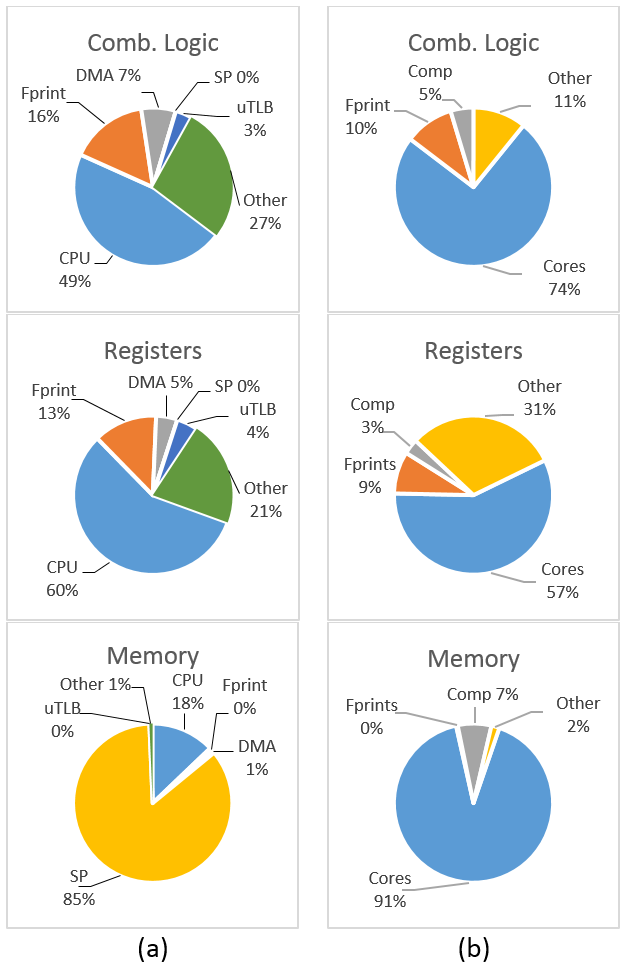
\includegraphics[scale=0.5]{figures/pie.png}
\caption[Fingerprinting FPGA resource allocation]{Fingerprinting FPGA overhead: (a) The local core and peripherals (b) The global system overhead}
\label{f:pie}
\end{figure}

	Figure \ref{f:pie}(b) shows the total cost of fingerprinting within a three core system where one core is assumed to be a reliable monitor and the two other cores are capable of fingerprinting.
	Therefore there are two fingerprinting units and a comparator added to the system.
	We note that the cost of the monitor core is probably too low because we have not implemented hardening or redundancy;
		this makes the relative cost of fingerprinting in this case pessimistic.
	The comparator represents only 6\% of combinationals, 4\% of registers and 7\% of onchip memory (excluding main memory).
	Note that the comparator is constant cost so long as the number of cores is less than 16, making this an upper limit cost;
		fingerprinting becomes more affordable the larger the number of cores that are supported.


\subsection{Single Task Replication and Detection Latency}

\begin{figure}[tb]
\centering
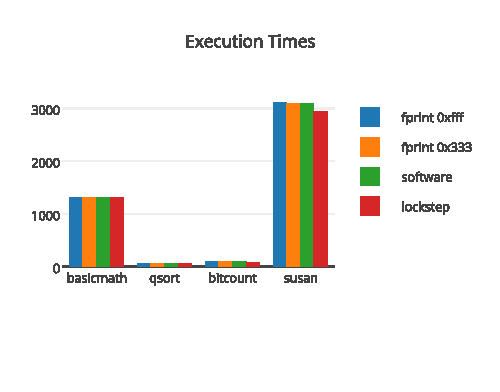
\includegraphics[scale=1.5]{Figures/execution_times}
\caption[Execution Time Results.]{\emph{Execution Time Results:} Four testbenches are executed on the three platforms. Fingerprinting is repeated with two different block sizes. There are no significant differences in execution time between any of the platforms.}
\label{f:extimes}
\end{figure}

	We compare the execution time of (a) lockstep DMR, (b) software voting, and (c) fingerprinting in Figure~\ref{f:extimes}.
	Fingerprinting is tested with two different block sizes.
	Execution time is measured from when the monitor first starts preparing the context of the other cores until it is notified that the task is completed, either by the comparator (under fingerprinting) or by the core themselves (under software voting).
	The performance of the fingerprinting and software checking platforms vary by less than 1\% for basicmath to 22\% for bitcount compared to the single core. The difference in execution time between fingerprinting and software checking is less than 1\% in all cases.
	The performance overhead associated with software checking and extra memory transactions (due to the fact that results must be copied from both cores) are not significant given the size of the data transfers compared to the lengths of the tasks.


\begin{figure}[tb]
\centering
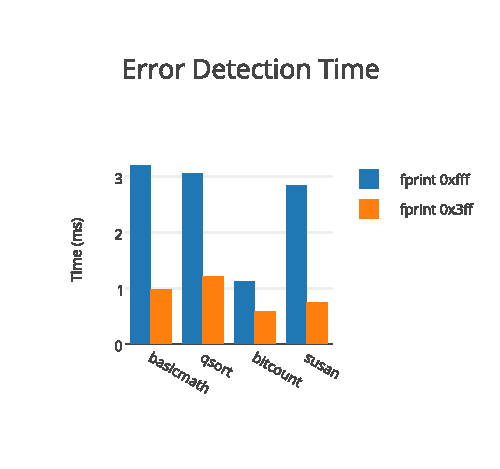
\includegraphics[scale=1.5]{Figures/error_detection_time}
\caption[Error detection latency]{The time it takes to detect an error with fingerprinting. Software voting cannot detect a fault until the task completes; lockstep DMR error detection latency varies based on implementation, but in some cases is no faster than fingerprinting.}
\label{f:dettimes}
\end{figure}

	In Figure~\ref{f:dettimes}, we report the error detection latency when one of the fingerprinted tasks is presented a faulty input.
	We observe that, as expected, the length of the fingerprinting block has an impact on detection latency.
	However, the placement of an error within a block and the density of store instructions will also have an effect.
	The bitcount testbench has such a different profile compared to the others because it uses bitwise operations as opposed to floating point which results in much more frequent pushing of data onto the stack. Furthermore, the erroneous input takes longer to affect the program execution.
		The detection latencies in Figure~\ref{f:dettimes} are significantly shorter than the execution times for a completed task; there is a potential to recover tens or even hundreds of extra milliseconds compared to software voting if a fault that occurs early in the execution of a task.
	
\subsection{Discussion}
	
	Consider again the Freescale Qorriva MPC577xK \cite{freescale2014qorivva} and Infineon Aurix 9x automotive ECUs \cite{infineon2014aurix} to place the resource utilization results in context. Firstly, a large amount of chip area on ECUs is devoted to interfacing with the external system. The Aurix chip, which is meant to be suited for several automotive applications that typically would have specialized ECUs, uses several serial bus controllers (e.g. I2C and Flex CAN), memory controllers, time management resources, interconnect logic, ADCs, and hardware security module. Secondly, the cores themselves are quite large and featured. The Qorriva Z7 cores have 16kB of instruction and data cache, 64 kB for data scratchpad, and FPUs. The lockstep functional safety core is also equipped with an FPU. Within this context, a fingerprint unit size of 30\% of the Nios core is quite reasonable. The Nios core we use has a 16kB scratchpad, 1kB instruction cache, no data cache or integer multiplication or division units and no MMU (future mixed criticality systems should expect to have full virtualization services to support hypervisors and more full-featured OS kernels such as Linux or Android). We argue that the comparison of fingerprint and CPU resource utilization on FPGA serves strictly as a rough measure demonstrating that the fingerprint unit is reasonably sized compared to the CPU and other peripherals that one might expect to find associated with each core. Furthermore, the size of comparator is reasonable taken against the size of the system when we consider that it supports up to 16 cores and that a realistic multicore ECU would be significantly larger than our prototype. Our platform excludes many peripherals and controllers such as IO interfaces, serial communication and memory controllers, ADC, PLL etc. 
	
	There are advantages to fingerprinting compared to core hardening techniques. While core hardening techniques exist that boast 10-15\% area overhead on custom CPU designs, they represent a a constant energy overhead whether the program running requires the higher reliability or not (i.e. they cannot be disabled). Furthermore, many core hardening techniques do not provide high enough coverage to support the most safety critical applications. Adoption of these techniques by manufacturers also poses a much greater risk since they require modifications to the CPU at the microarchitectural level. Fingerprinting is a non-invasive technique that can be integrated into a system without modifying the ISA or the CPU. Code can be written to be successfully fingerprinted without modifying the compiler toolchain or changing the code style from MISRA standards. We believe that fingerprinting is an ideal technique to be integrated into the automated design space exploration and code generation model-based design methodology because it provides several runtime tunable parameters and can be completely disabled.
	
	The main advantage of fingerprinting with respect to software checking and voting is the potential to greatly reduce detection latencies. Task level software checking suffers from large detection latency and increased memory transactions (although in the testbenches we examined these extra memory transactions were negligible). Single threaded software checking implemented by the compiler causes performance of the task to suffer and requires toolchain support (not tested in this paper but shown elsewhere). Multicore fault tolerant schedules require contingency plans in the case of failure. Fingerprinting reduces detection latencies which should eliminate the need for task grouping (which is done to reduce the overhead of voting and checking tasks) and can simplify the search for alternative schedules in the presence of multiple faults. Fingerprinting also has little to no impact on the performance of the task. Fingerprinting may cause very minor interference if it must use global buses to send information to the comparator. However these effects should be mitigated in a system with a deterministic (e.g. TDM) bus policy.	 
	
	
 

%----------------------------------------------------------------------------------------
%	THESIS CONTENT - APPENDICES
%----------------------------------------------------------------------------------------

\appendix % Cue to tell LaTeX that the following "chapters" are Appendices

% Include the appendices of the thesis as separate files from the Appendices folder
% Uncomment the lines as you write the Appendices

% Appendix A

\chapter{User Configuration File} % Main appendix title

\label{A:ConfigFile} % For referencing this appendix elsewhere, use \ref{AppendixA}


The configuration file provided to the program must be able to express the basic flow as well as leave open the possibility of integrating extensions in the future. The syntax should be both easy to read for the user while also being easy to parse.

First, the functions must be specified. Each function must have a root name, a directory location as well as a constructor for global variables. The naming conventions for function names will follow the convention for Simulink generated code. The folder must contain the \texttt{ert\_main.c} file that provides variable declarations and initialization code.

The configuration file will be specified through examples. First, the function declarations:

\begin{lstlisting}[caption={Function configuration syntax},label=l:config-function,language=bash]
#periodic tasks, some are critical, all independent (no dataflow between tasks)


#function list must come first!!

#Comments start with #
# -c for critical task
# -T for task period in ms
# -E for event driven, runs when all the inputs are available
# -S for stacksize, if S is not present then assume profiler was used
# 	if profiler was used: should have a profile.log file in the function folders
<FUNCTIONLIST>
-rootdir /home/jonah/fingerprinting/automotive_control/CompiledC/for_loops
-name for_loop_100000_0    -subdir for_loop_100000_0           -T  30   -c  -Priority 2	
-name for_loop_50000_50000 -subdir for_loop_50000_50000		   -T  30       -Priority 1 -printRuntime -addPreamble preamble.txt
</FUNCTIONLIST>

#preamble -> in subdir folder, contains code to go before while loop in task, used for threadsafe newlib config, should not have extension .c or .h
#printRuntime adds diagnostic printf run time for the given task

<DATAFLOW>
</DATAFLOW>


<PLATFORM>
-usedefault
</PLATFORM>

<MAPPING>
for_loop_100000_0 cpu0 cpu1
for_loop_50000_50000 cpu0
</MAPPING>

#optional - skip stack profiling if included
<STACK_PROFILE>
for_loop_100000_0 80
for_loop_50000_50000 80
</STACK_PROFILE>


#optional - skip wcet profiling if included
<WCET_PROFILE>
for_loop_50000_50000 1600035
for_loop_100000_0 1600004 2400006
</WCET_PROFILE>
\end{lstlisting}


Whitespace is ignored except for line breaks. Each top level function must have a unique name and only be instantiated once.

%\input{Appendices/AppendixB}
%\input{Appendices/AppendixC}

%----------------------------------------------------------------------------------------
%	BIBLIOGRAPHY
%----------------------------------------------------------------------------------------
\printbibliography[heading=bibintoc]

%----------------------------------------------------------------------------------------

\end{document}  
